\documentclass{beamer}
\usepackage[utf8]{inputenc}
\usepackage{algorithm,algpseudocode}
\usepackage{xmpmulti}
\usepackage{listings}
\usepackage{booktabs}
\usepackage{nicefrac}
\usepackage{pgfplots}
\usepackage{amssymb}
\usepackage{amsmath}
\usepackage{tikz}
\usepackage{bbm}
\usepackage{bm}
\usepackage{enumitem}
\usepackage{hyperref}
\usepackage[export]{adjustbox}
\usepackage{svg}

\usetheme{Madrid}
\definecolor{mlpblue}{rgb}{0.1, 0.14, 0.24}

\pgfplotsset{colormap={mine}{[1cm] rgb255(0cm)=(255,0,0) rgb255(1cm)=(0,0,255)}}

\useoutertheme{infolines} % Alternatively: miniframes, infolines, split
\useinnertheme{circles}
\usecolortheme[named=mlpblue]{structure}

\lstset{basicstyle=\footnotesize\ttfamily,breaklines=true}

%------------------------------------------------------------
%This block of code defines the information to appear in the
%Title page
\title[Optimal Transport]{Introduction to Optimal Transport\thanks{\href{https://arxiv.org/abs/1803.00567}{Peyré, Cuturi.~[Arxiv 2020]}}\thanks{\href{https://arxiv.org/abs/1701.07875}{Arjovsky, et.~al.~[Arxiv 2017]}}\thanks{\href{https://arxiv.org/abs/2006.07229}{Heitz, et.~al.~[CVPR 2021]}}}

\subtitle{``Moving Sandcastles in the Air''}

\author[ECE ML Reading Group] % optional
{J.~Setpal} 

\date{March 26, 2025}

\titlegraphic{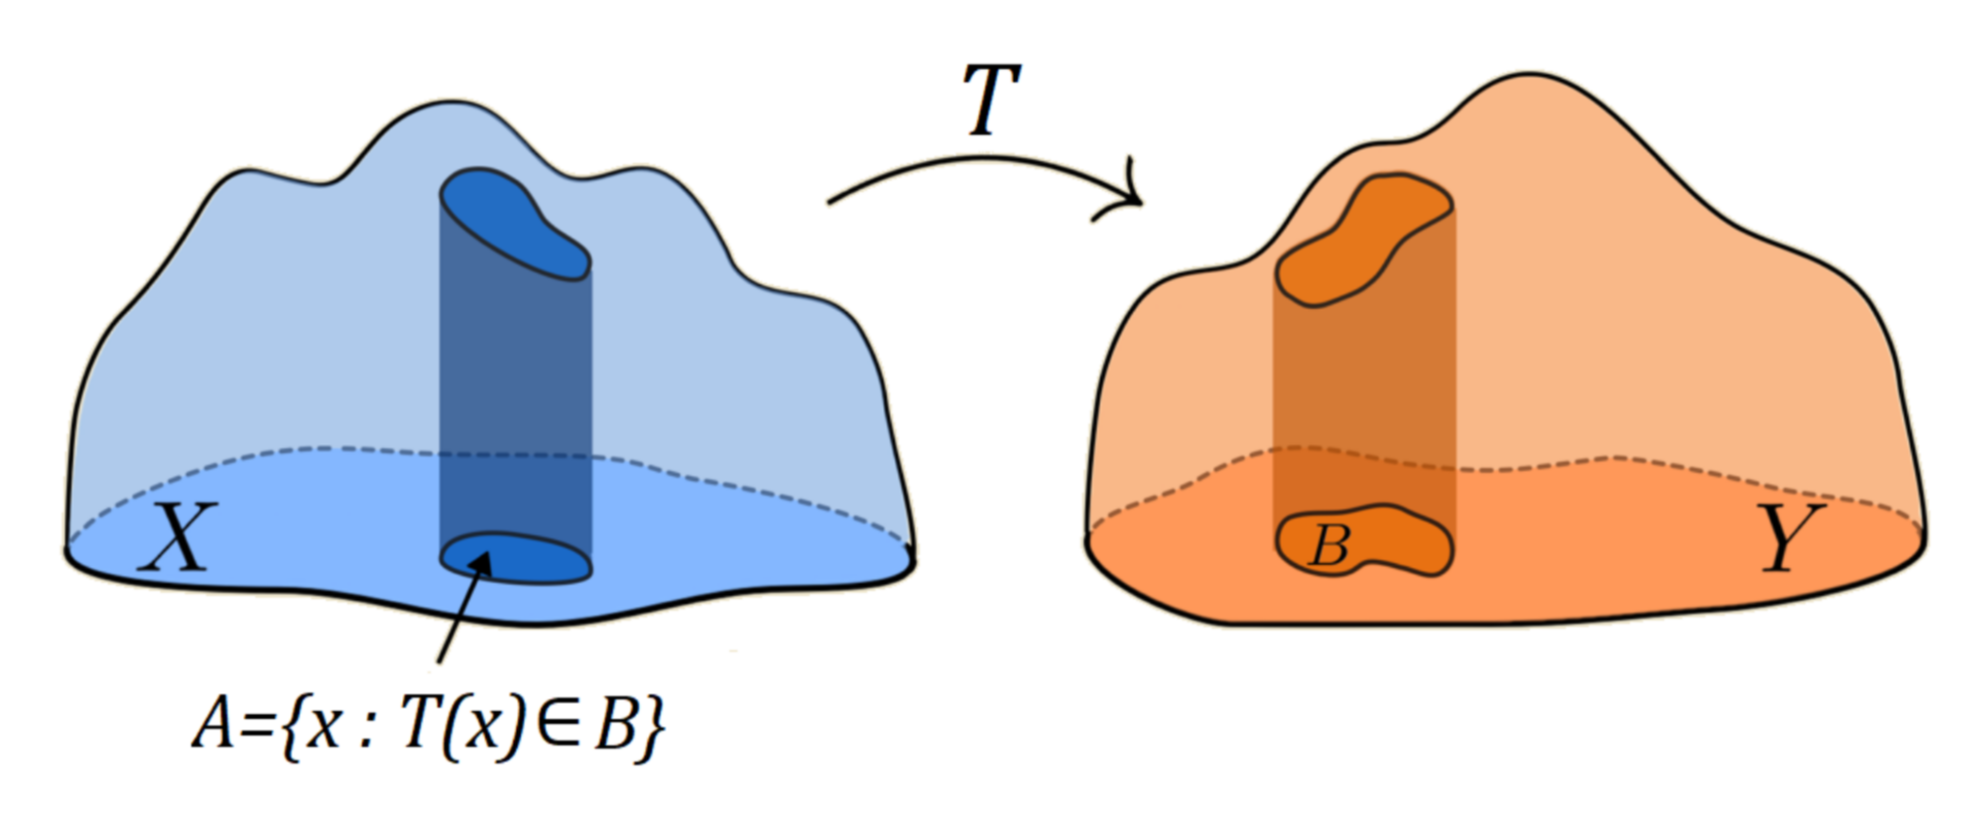
\includegraphics[width=6cm]{img/mrmonge.png}}

%End of title page configuration block
%------------------------------------------------------------

%The next block of commands puts the table of contents at the 
%beginning of each section and highlights the current section:

\AtBeginSection[]
{
  \begin{frame}
    \frametitle{Outline}
    \tableofcontents[currentsection]
  \end{frame}
}
% ------------------------------------------------------------


\begin{document}

\frame{\titlepage}


%---------------------------------------------------------
% This block of code is for the table of contents after
% the title page
\begin{frame}
\frametitle{Outline}
\tableofcontents
\end{frame}
%---------------------------------------------------------

\section{Motivation}

\begin{frame}{Why Should We Care? ($\nicefrac{1}{3}$)}
	Monge likes playing with sandcastles. \newline \\

	He wonders, ``What is the most efficient way to move this marvellous sandcastle from the beach to my house?'' \newline \\

	And \textbf{Optimal Transport} was born. \pause \newline \\

	Why should you care:
	\begin{enumerate}[label=\arabic*.]
		\item You like playing with sandcastles. \pause
		\item You're interested in any of the following research foci:
			\begin{enumerate}[label=\alph*.]
				\item \bf Neural Style Transfer:
					\begin{center}
						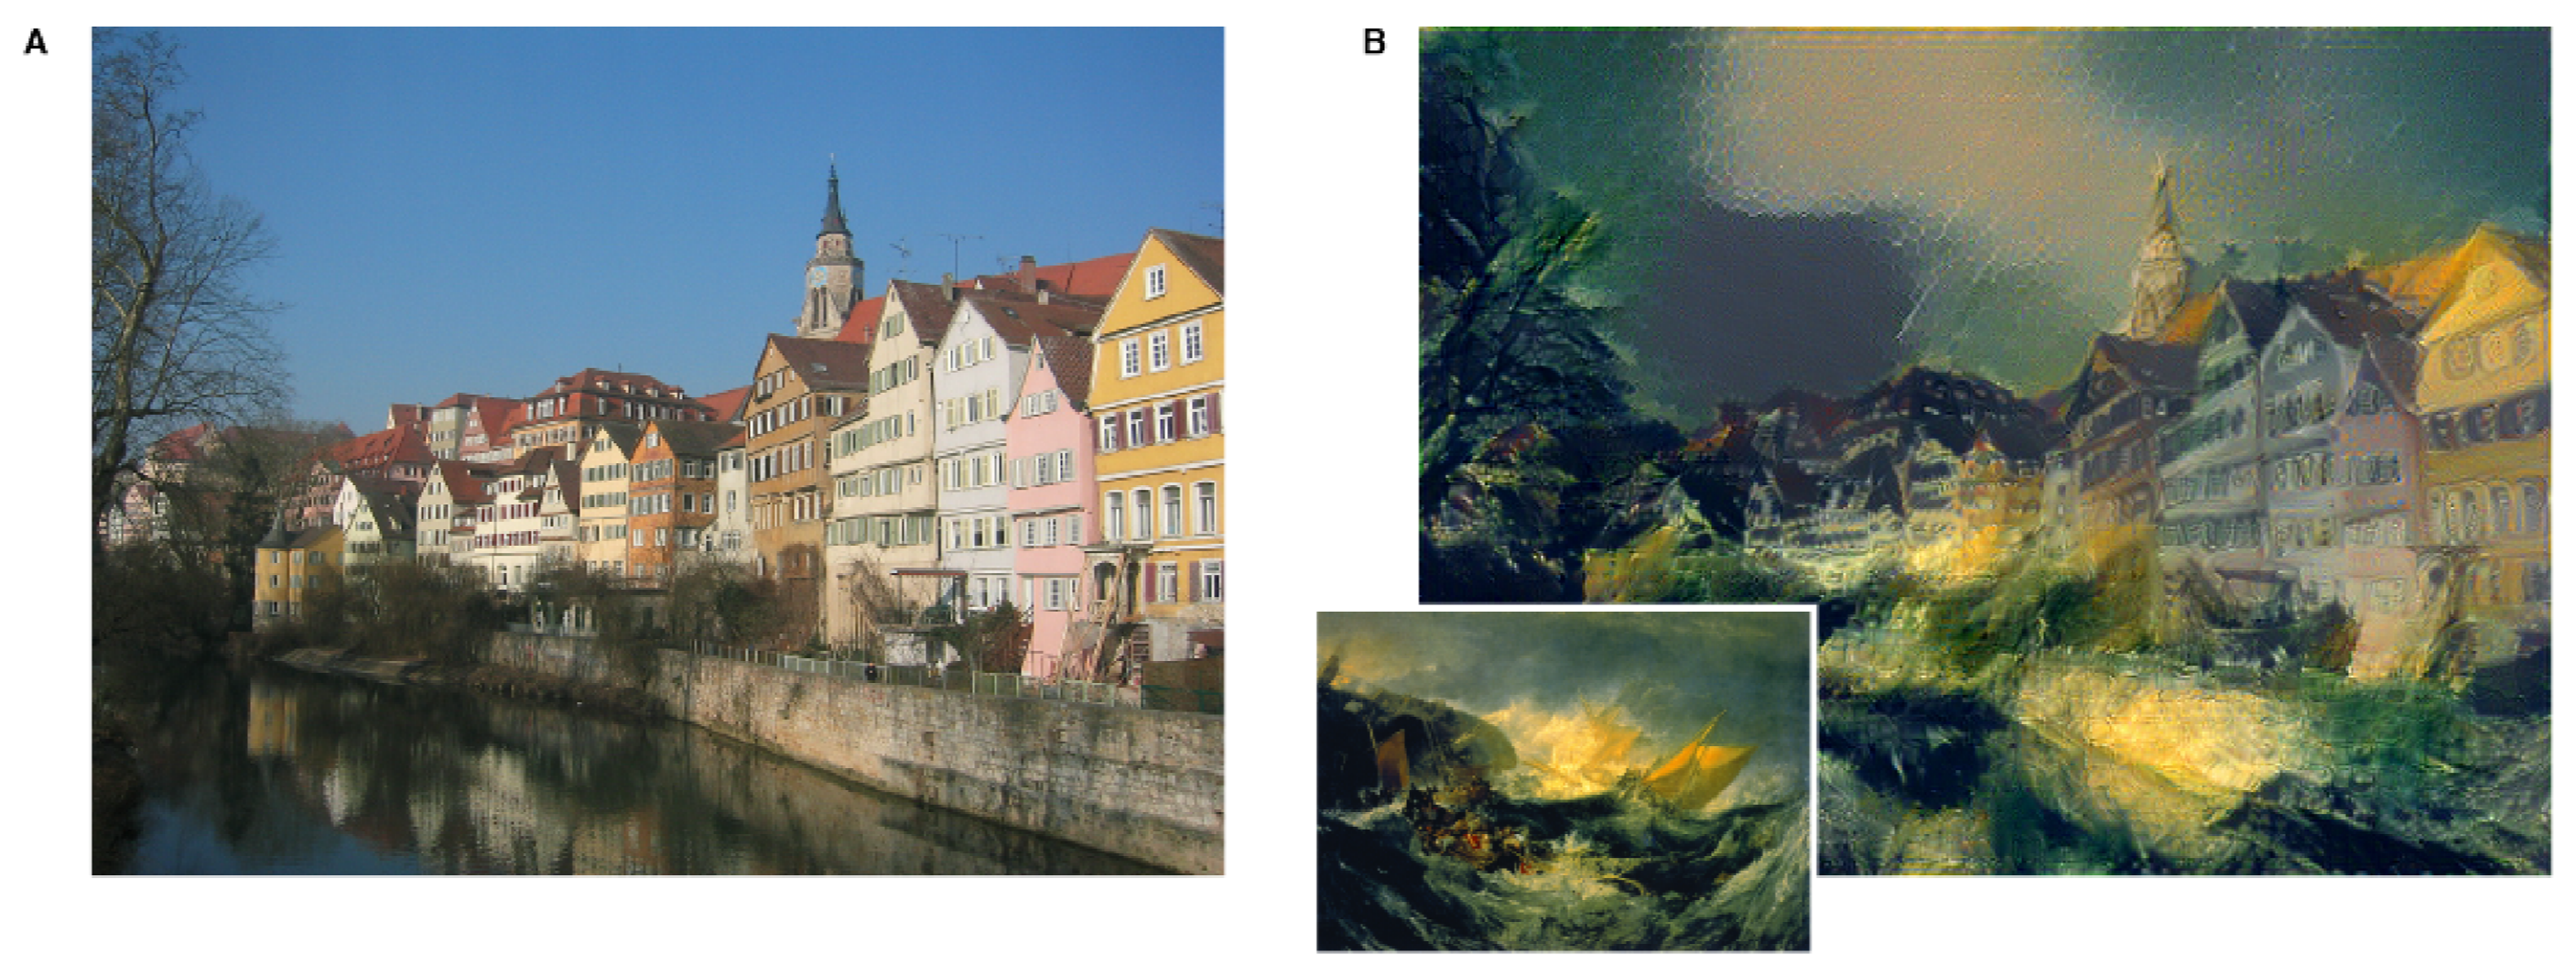
\includegraphics[width=.6\textwidth]{img/styletransfer.png}
					\end{center}
			\end{enumerate}
	\end{enumerate}
\end{frame}

\begin{frame}{Why Should We Care? ($\nicefrac{2}{3}$)}
	\begin{enumerate}[label=\arabic*.]
		\setcounter{enumi}{1}
		\item
			\begin{enumerate}[label=\alph*.]
				\setcounter{enumii}{1}
				\item \textbf{Sentence Similarity} (Word Mover's Distance):
					\begin{center}
						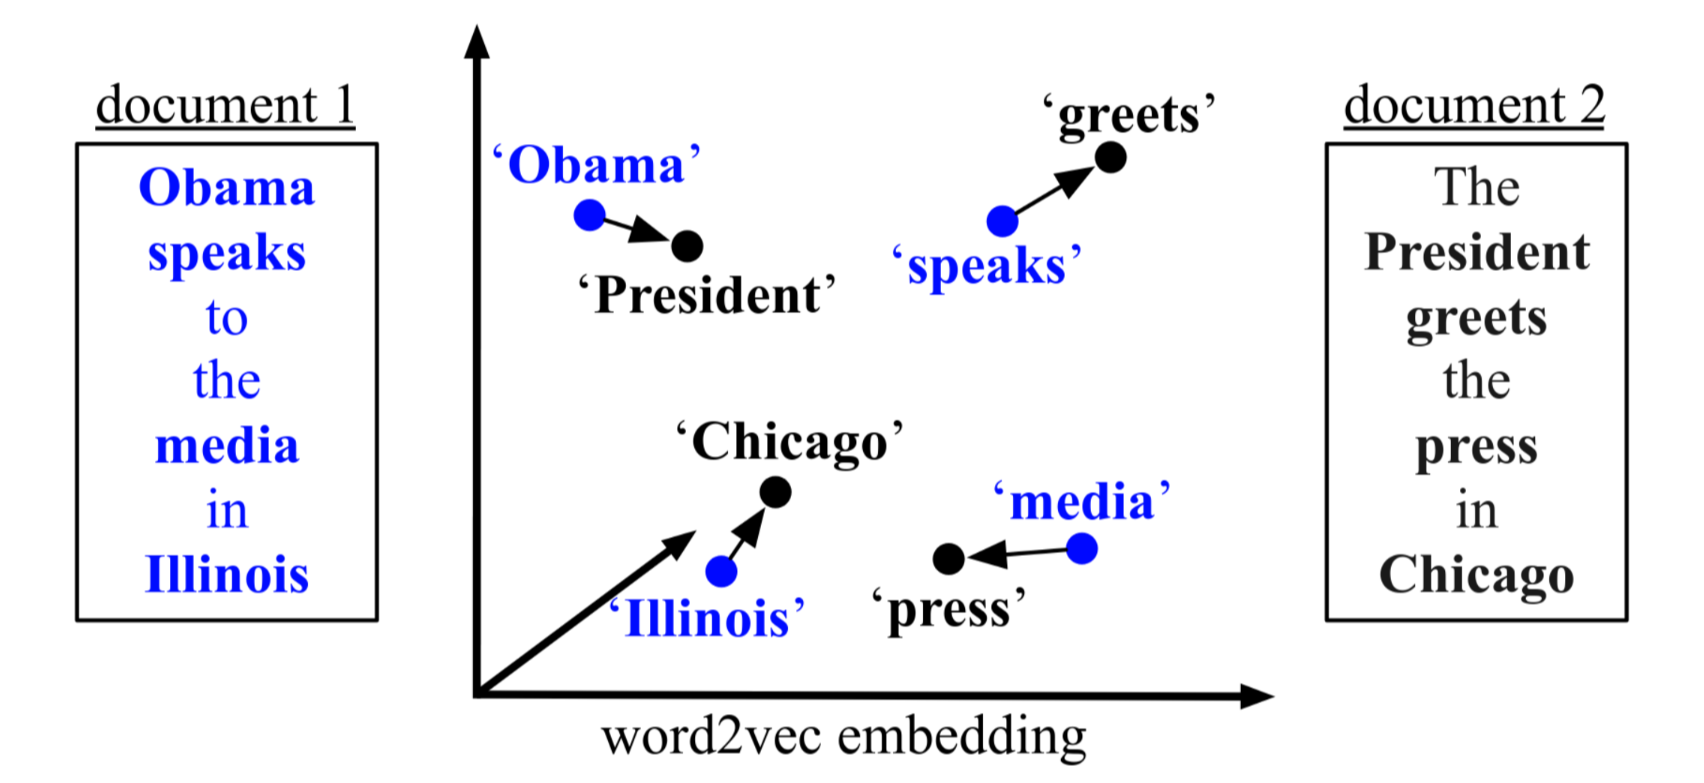
\includegraphics[width=.6\textwidth]{img/wmd.png}
					\end{center} \pause
				\item \textbf{Graph Neural Networks} (Better Representation Learning):
					\begin{center}
						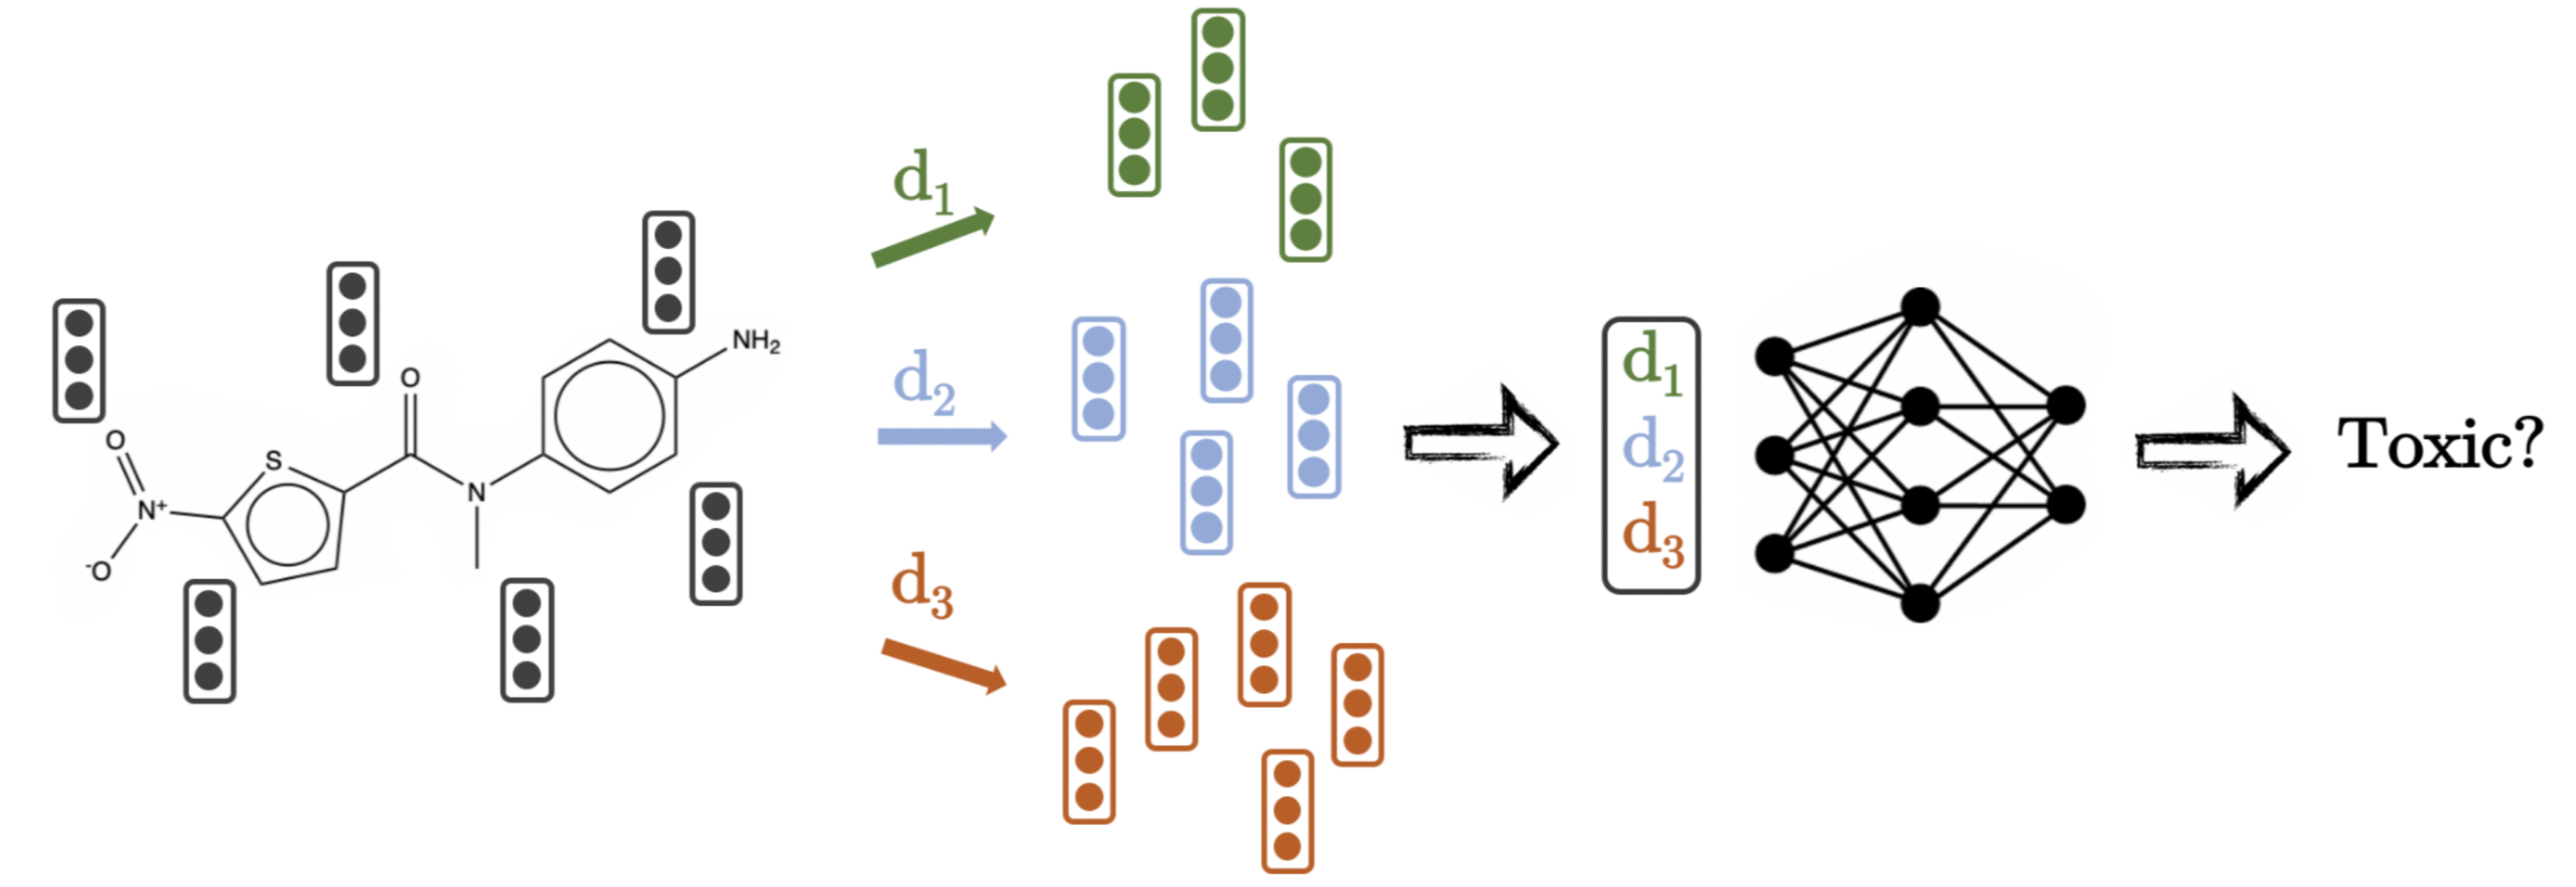
\includegraphics[width=.7\textwidth]{img/gnn.png}
					\end{center}
			\end{enumerate}
	\end{enumerate}
\end{frame}

\begin{frame}{Why Should We Care? ($\nicefrac{3}{3}$)}
	\begin{enumerate}[label=\arabic*.]
		\setcounter{enumi}{1}
		\item
			\begin{enumerate}[label=\alph*.]
			\setcounter{enumii}{3}
				\item \textbf{Medical Imaging} (Gray Matter Tissue loss for Dementia):
					\begin{center}
						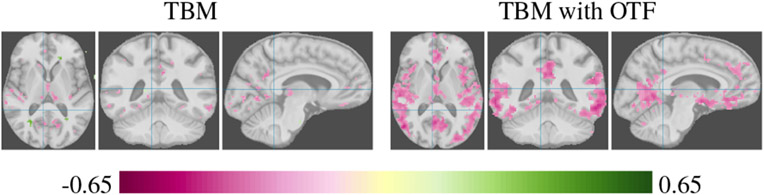
\includegraphics[width=.8\textwidth]{img/ctscan.jpg}
					\end{center} \pause
					\vspace{1.5em}
				\item \bf Robust Point-Cloud Matching:
					\begin{center}
						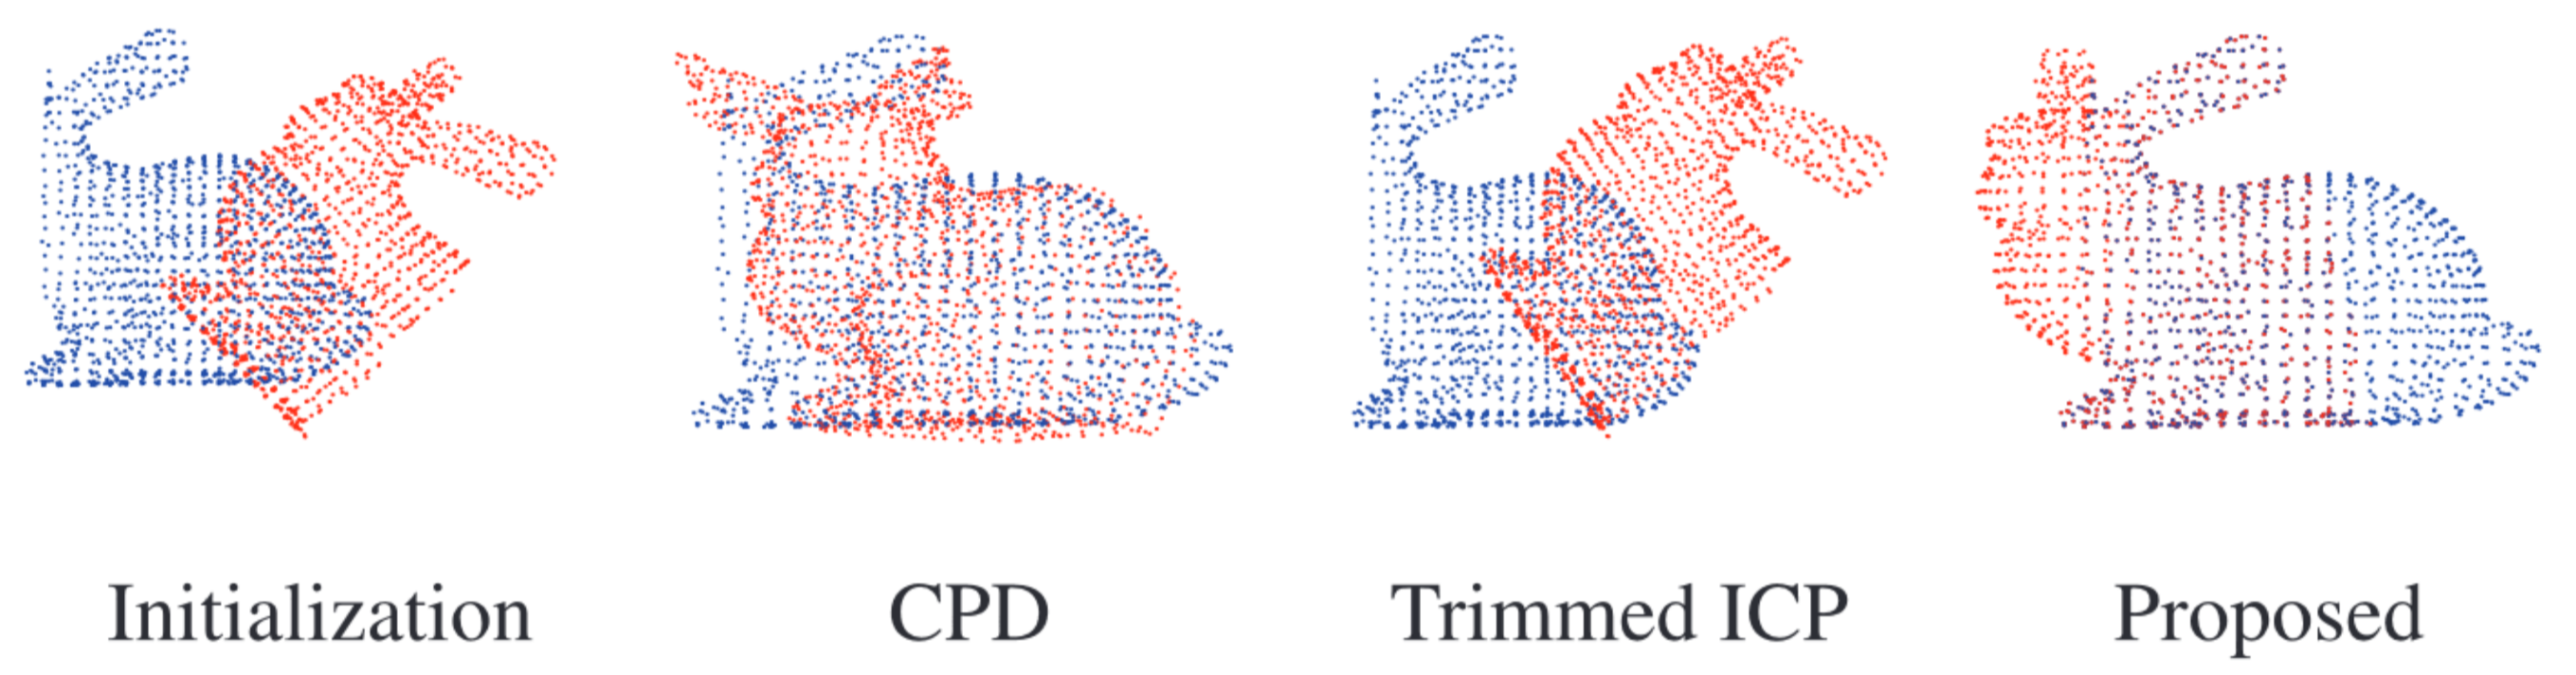
\includegraphics[width=.8\textwidth]{img/pcm.png}
					\end{center}
			\end{enumerate}
	\end{enumerate}
\end{frame}

\section{Monge Problem, Kantorovich Relaxation}

\begin{frame}{Geometry Induced by OT on the Probability Simplex}
	We start with the probability simplex:
	\begin{gather}
		\Sigma_n := \left\{ \bm{a} \in \mathbb{R}^n_+ : \sum^n_{i=1} \bm{a}_i = 1 \right\}
	\end{gather} \pause

	Over which we define a discrete probability measure:
	\begin{gather}
		\alpha(x) = \sum^n_{i=1} \bm{a}_i \chi_{x_i}(x), \quad \text{s.t.} \quad \bm{a} \in \Sigma_n
	\end{gather} \pause

	\begin{block}{\bf Aside}
		OT literature deals with both discrete and continuous measures using the same framework. We'll focus mostly on the discrete setting.
	\end{block}
\end{frame}

\begin{frame}{Monge's Assignment Problem ($\nicefrac{1}{2}$)}
	Monge asks us to transfer measure $\alpha$ to a new measure $\beta$ while also \underline{minimizing the total cost of transportation}.
	\begin{gather}
		\alpha(x) = \sum^n_{i=1} \bm{a}_i \chi_{x_i}(x), \quad \beta(y) = \sum^m_{i=1} \bm{b}_i \chi_{y_i}(y)
	\end{gather} \pause
	To quantify cost we have matrix $\bm{C} \in \mathbb{R}^{n \times m}$ which determines the cost of moving mass $x_i \rightarrow y_j~\forall i,j \in \{1, \ldots, n\}, \{1, \ldots, m\}$. \pause \newline \\
	We define a map $T: \mathcal{X} \rightarrow \mathcal{Y}$ that tells us what to move where. This is our \textbf{Transport Plan}. \pause Now, we can formally define the assignment objective:
	\begin{gather}
		\min_{T} \frac{1}{n} \sum^n_{i=1} \bm{C}_{i, T(i)}
	\end{gather} \pause
	If $n = m,~T \in \text{Perm}(n)$.
\end{frame}

\begin{frame}{Monge's Assignment Problem ($\nicefrac{2}{2}$)}
	Two visual examples of optimal transport:
	\begin{center}
		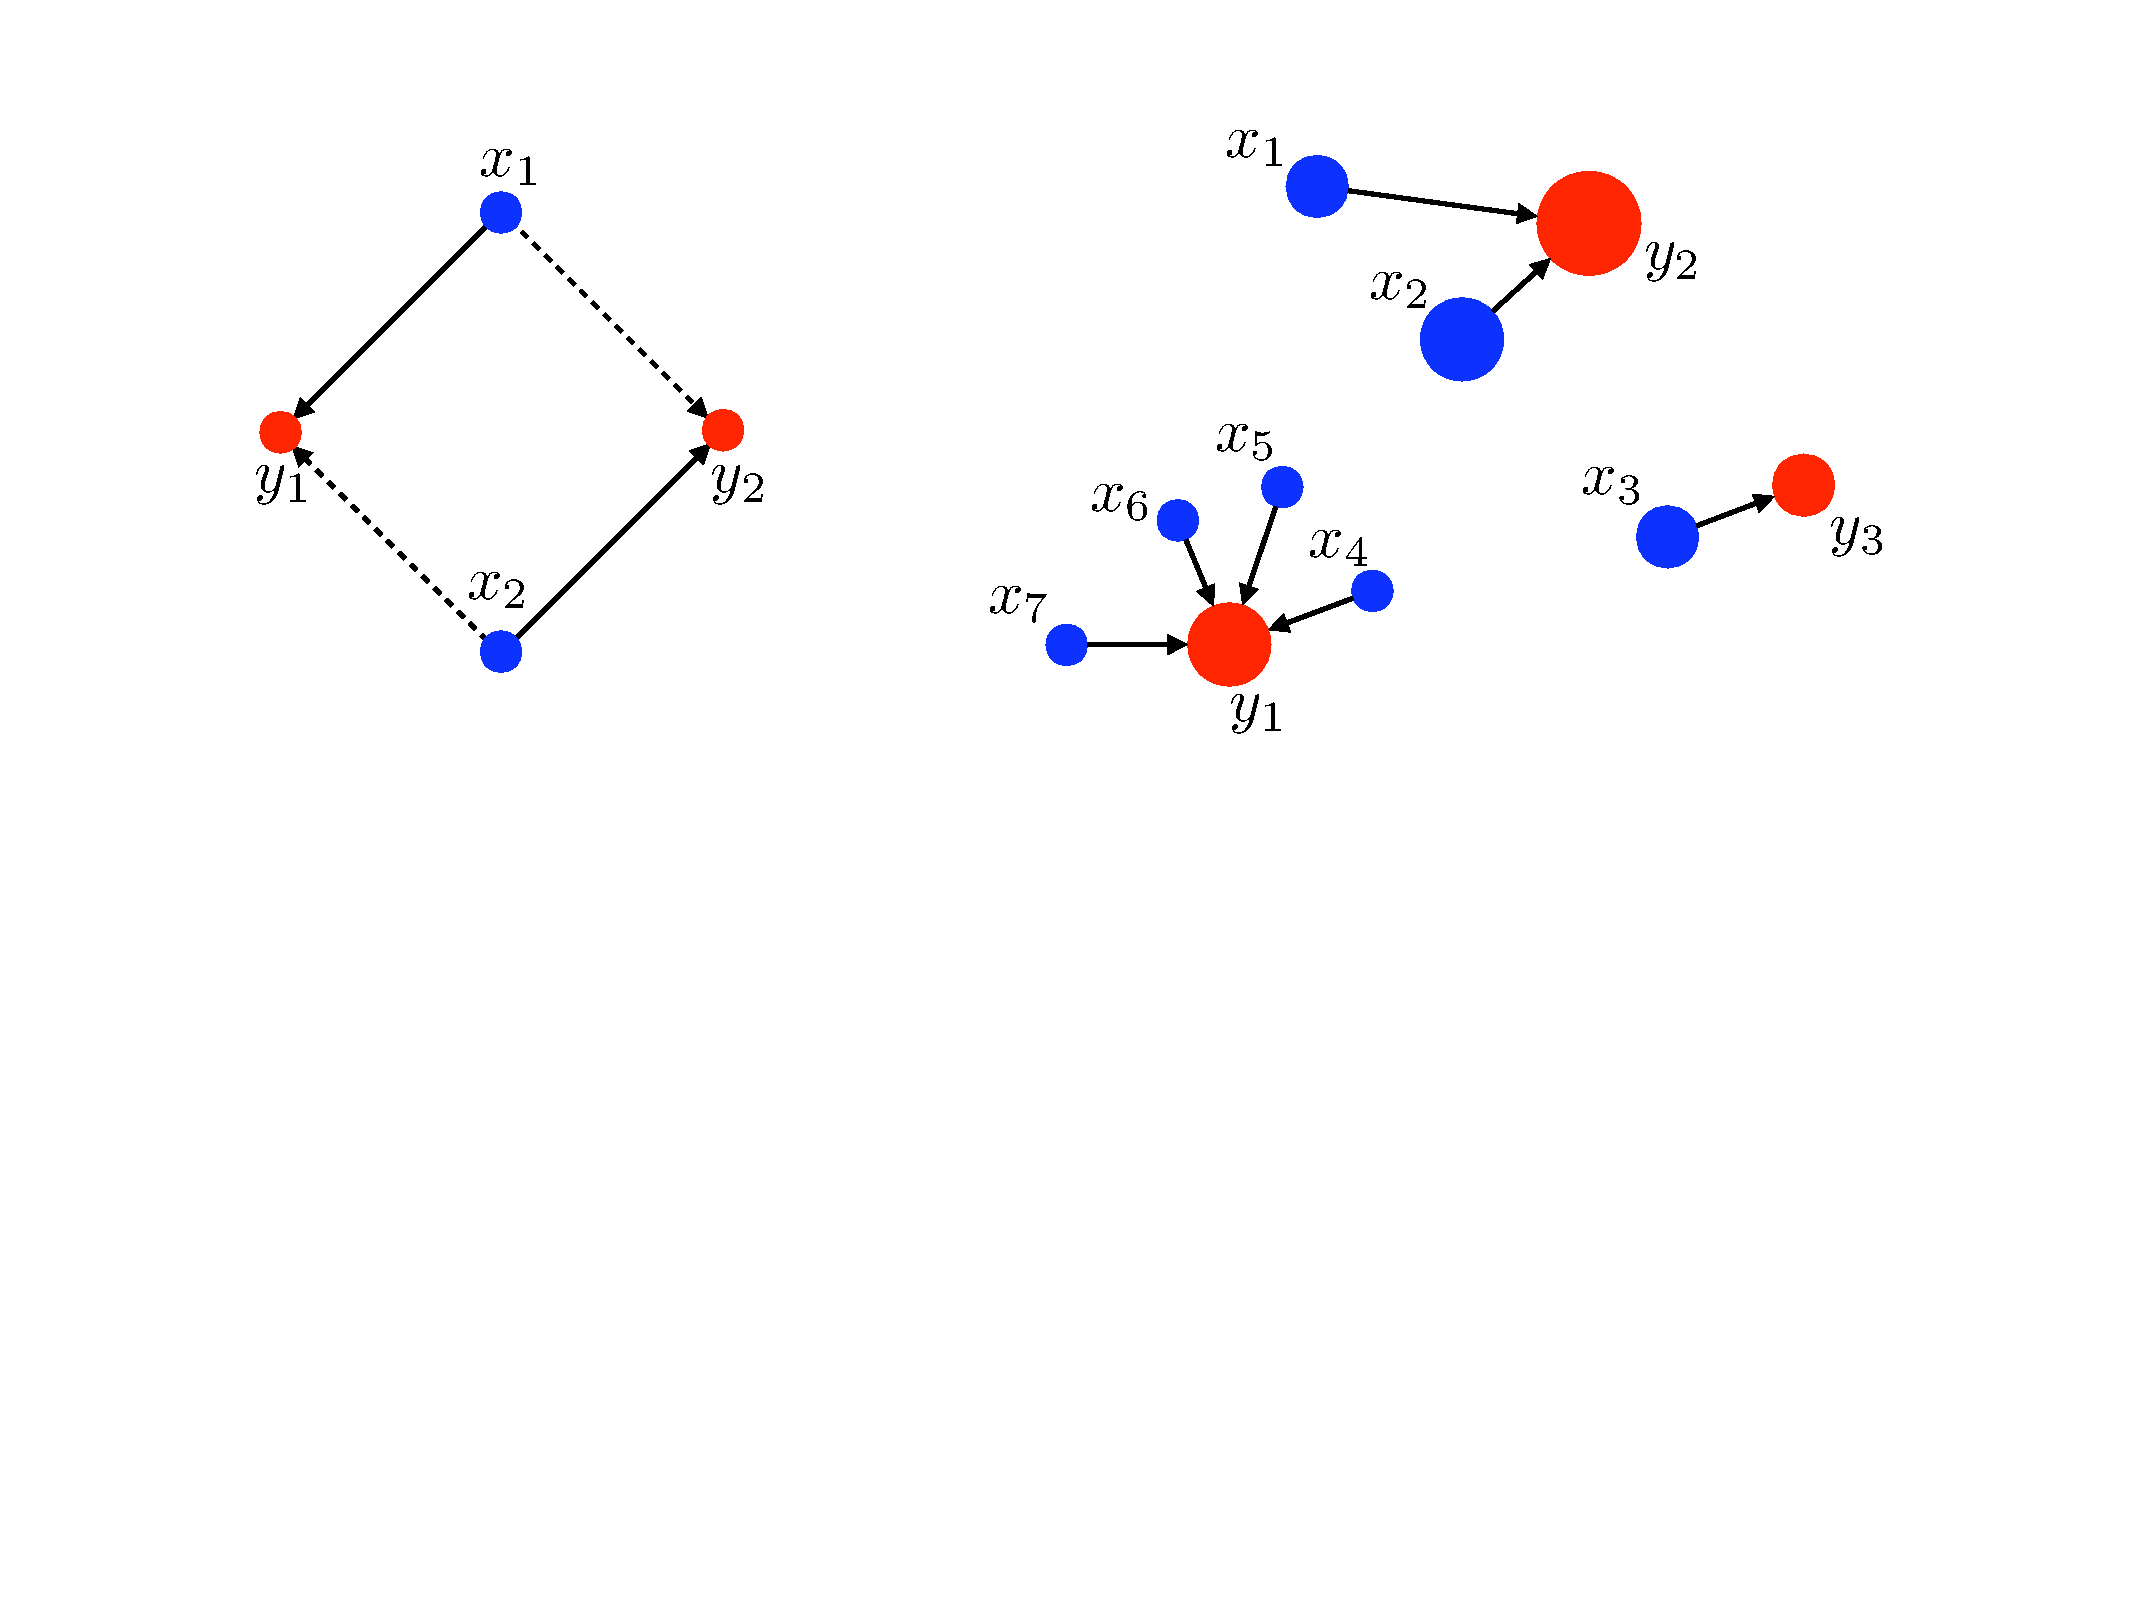
\includegraphics[width=.8\textwidth]{img/non-unique-optimal-matching}
	\end{center} \pause
	\textbf{Observations:}
	\begin{enumerate}[label=\arabic*.]
		\item The optimal transport map is not necessarily unique. \pause
		\item The current formulation does not allow mass-splitting. \pause
		\item If $m > n$ there is no feasible transport plan. \pause
		\item Complexity scales sharply and optimization landscape is non-convex.
	\end{enumerate}
\end{frame}

\begin{frame}{Push-Forward \& Pull-Back Operators}
	For every valid transport map, we know that the following is satisfied:
	\begin{gather}
		\forall j \in \{1, \ldots, m\}, \quad \bm{b}_j = \sum_{i : T(i) = y_j} \bm{a}_i
	\end{gather} \pause
	We define the \textbf{Push-Forward operator} $T_\sharp$ to map a transport plan over an entire measure space.
	\begin{gather}
		T_\sharp: \mathcal{M}(X) \rightarrow \mathcal{M}(Y), \quad \beta = T_\sharp \alpha := \sum_i^n \bm{a}_i \chi_{T(x_i)}
	\end{gather} \pause
	The Push-Forward operator is `different' from a composition on $T$. That is the \textbf{Pull-Back operator}:
	\begin{gather}
		T^\sharp: \mathcal{C}(\mathcal{Y}) \rightarrow \mathcal{C}(\mathcal{X}), \quad T^\sharp g := g \circ T
	\end{gather} \pause
	Push-Forward and Pull-Back operators are related as follows:
	\begin{gather}
		\forall (\alpha, g) \in \mathcal{M}(\mathcal{X}) \times \mathcal{C}(\mathcal{Y}), \quad \int_\mathcal{Y} g d (T_\sharp \alpha) = \int_{\mathcal{X}} T^\sharp g d \alpha
	\end{gather}
\end{frame}

\begin{frame}{Kantorovich Relaxation ($\nicefrac{1}{2}$)}
	Kantorovich saw slide 10 of this presentation in the 1940's and decided to take matters in his own hands. \pause \newline \\

	\textbf{Key Idea:} Relax determinism constraint $\rightarrow$ get probabilistic transport. \pause \newline \\

	Basically, we \underline{allow mass splitting}. \pause Instead of a transport map, we define a family of coupling matrices where each $\bm{P} \in \mathbb{R}^{n \times m}_+$ is a valid coupling:
	\begin{gather}
		\mathcal{U}(\bm{a}, \bm{b}) := \left\{ \bm{P} \in \mathbb{R}^{n \times m}_+ : \underbrace{\bm{P} \mathbbm{1}_m = \bm{a}, \bm{P}^T \mathbbm{1}_n = \bm{b}}_{\text{mass conservation}} \right\}
	\end{gather} \pause
	Finally, our new optimization objective is as follows:
	\begin{gather}
		L_{\bm{C}}(a, b) := \min_{\bm{P} \in \mathcal{U}(a, b)} \langle \bm{C}, \bm{P} \rangle_F = \sum_{i, j} \bm{C}_{i,j} \bm{P}_{i, j}
	\end{gather} \pause

	\textbf{BIG Observation:} This is a linear program.
\end{frame}

\begin{frame}{Kantorovich Relaxation ($\nicefrac{2}{2}$)}
	\begin{figure}[h!]
		\centering
		\begin{tabular}{@{}c@{\hspace{5mm}}c@{}}
			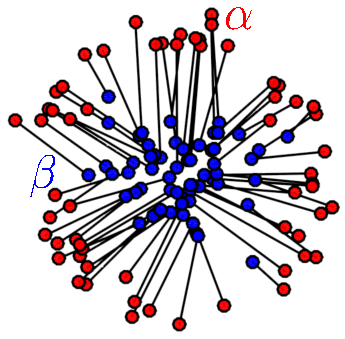
\includegraphics[width=.3\textwidth]{img/matching-kantorovitch/matching}&
			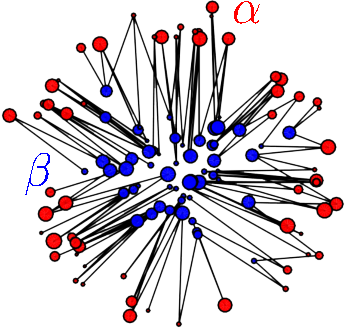
\includegraphics[width=.3\textwidth]{img/matching-kantorovitch/weighted}
		\end{tabular}
	\end{figure} \pause
	\vspace{-1.5em}
	\textbf{Observations:}
	\begin{enumerate}[label=\arabic*.]
		\item If we restrict $\bm{P}$ to the permutation matrix and have each weight be uniform, we recover Monge maps. \pause This restriction further implies:
			\begin{gather}
				L_{\bm{C}}(\nicefrac{\mathbbm{1}_n}{n}, \nicefrac{\mathbbm{1}_n}{n}) \leq \min_{T \in \text{Perm}(n)} \langle \bm{C}, \bm{P}_T \rangle
			\end{gather} \pause
			So, the Kantorovich Relaxation is \textbf{tight}. \pause
		\item Each coupling $\bm{P}$ is symmetric: $\bm{P} \in \mathcal{U}(\bm{a}, \bm{b}) \iff \bm{P}^T \in \mathcal{U}(\bm{a}, \bm{b})$.
	\end{enumerate}
\end{frame}

\section{Kantorovich Problem's Dual Formulation}

\begin{frame}{Implications of Linear Programs}
	The headline news from the Kantorovich Relaxation is that \textbf{our optimization objective is now a linear program}. \pause \newline \\

	So what are the implications of this?
	\begin{enumerate}[label=\arabic*.]
		\item Can be solved in $\mathcal{O}(n^{2.5} \log n)$. \pause
		\item The OT problem is now convex. \pause
		\item The OT problem has a \textit{dual}, which is a linear program whose optimal value \underline{upper bounds} the optimal value of the primal. \pause
		\item The optimal value for the primal problem \textit{equals} the dual $\iff$ the program has an optimal solution -- by \textbf{Strong Duality Theorem}. \pause
		\item If we know an optimal solution exists, we can choose to solve the easier problem and get the same answer.
	\end{enumerate}
\end{frame}

\begin{frame}{Kantorovich Dual}

The Kantorovich problem is a constrained convex minimization problem, while the dual is a constrained concave maximization  problem. \pause \newline \\

Like the primal, we still must define a feasible set:
\begin{gather}
	\mathcal{R}(\bm{C}) := \{ (\bm{f}, \bm{g}) \in \mathbb{R}^n \times \mathbb{R}^m : \bm{f} \oplus \bm{g} \leq \bm{C}\}
\end{gather} \pause

From there, we have the following dual problem:
\begin{gather}
	L_{\bm{C}}(\bm{a}, \bm{b}) = \max_{\bm{f}, \bm{g} \in \mathcal{R}(\bm{C})} \langle \bm{f}, \bm{a} \rangle + \langle \bm{g}, \bm{b} \rangle
\end{gather}

	The dual variables, here $\bm{f}, \bm{g}$ are called \underline{Kantorovich Potentials}.
\end{frame}

\begin{frame}{Intuitive Example of the Dual in Practice}
	Consider a hypothetical where an operator wants to transfer goods from warehouses to factories. \pause \newline \\

	One way to optimize costs would be to plan a route, by solving $L_{\bm{C}}(\bm{a}, \bm{b})$. \newline \\

	If the optimal plan is too expensive to compute, what can be done? \pause \newline \\

	One solution could be to \textit{outsource}. A vendor may present dual variables:
	\begin{align}
		\bm{f} &= \begin{bmatrix} \text{unit cost of pickup from warehouse}~i \end{bmatrix}^T \\
		\bm{g} &= \begin{bmatrix} \text{unit cost to deliver to factory}~j \end{bmatrix}^T 
	\end{align} \pause
	To check the optimality of the vendor's prices, the operator can use $\bm{C}_{i,j}$:
	\begin{gather}
		\forall (i,j), \quad \bm{f}_i + \bm{g}_j \stackrel{?}{\leq} \bm{C}_{i,j} 
	\end{gather}
\end{frame}

\section{Optimal Transport Induces a Distance}

\begin{frame}{$p$-Wasserstein Distance ($\nicefrac{1}{2}$)}
	If we fix $\bm{C}$, we can compare measures / histograms by the cost of transporting a measure / histogram to the other. \pause \newline \\
	
	We will consider $p$-norms for our cost computation: $\bm{C}_{i,j} = \| x_i  - y_j \|_p$ \pause \newline \\

	Crucially, the optimal transport cost satisfies properties of a \underline{distance}. \pause \newline \\

	Let $n = m,~p \geq 1, \bm{C} = \bm{D}^p = (\bm{D}^p_{i, j})_{i,j} \in \mathbb{R}^{n \times n}$. We can verify:
	\begin{enumerate}[label=\arabic*.]
		\item $\bm{D} \in \mathbb{R}^{n \times n}_+$ is symmetric. \pause
		\item $\bm{D}_{i,j} = 0 \iff i = j$ \pause
		\item $\forall (i, j, k) \in \{1, \ldots, n\},~\bm{D}_{i,k} \leq \bm{D}_{i, j} + \bm{D}_{j, k}$ \pause
	\end{enumerate}
	~ \\
	Using this, we define the \textbf{Wasserstein Distance}:
	\begin{gather}
		W_p (\bm{a}, \bm{b}) := L_{\bm{D}^p}(\bm{a}, \bm{b})^{\nicefrac{1}{p}}
	\end{gather}
\end{frame}

\begin{frame}{$p$-Wasserstein Distance ($\nicefrac{2}{2}$)}
	No visual this time, but we still have \textbf{observations}:
	\begin{enumerate}[label=\arabic*.]
		\item $W_p$ is expensive to compute; there is no closed-form solution. \pause
		\item $W_p$ `lifts' $L_p$ distance from points to measures / histograms. \pause
		\item (Not obvious) Over Euclidean space, we can \textbf{factor out translations}. \pause \newline \\
			Let $T_\tau : x \mapsto x - \tau$ be the translation operator, $\bm{m}_\gamma := \int_{\mathcal{X}} x~d\gamma$ be the mean of measure $\gamma$. Now, we then have:
			\begin{gather}
				W_2({T_\tau}_{\sharp} \alpha, {T_{\tau'}}_{\sharp} \beta)^2 = W_2(\tilde{\alpha}, \tilde{\beta})^2 + \| \bm{m}_\alpha - \bm{m}_\beta \|^2
			\end{gather}
			Where $(\tilde{\alpha}, \tilde{\beta})$ are zero-centered versions of measures $(\alpha, \beta)$. \pause \newline \\
			This distinction implies a two-fold comparison: the shapes of measures $\alpha$ and $\beta$, and the distance between their means.
	\end{enumerate}
\end{frame}

\begin{frame}{Sliced Wasserstein Distance ($\nicefrac{1}{4}$)}
	One special case of Optimal Transport is the 1-D case; $\mathcal{X} = \mathbb{R}$. Assuming uniform weights\footnote{generic case is more involved, but idea still holds.} and $c(x, y) = \| x - y \|^p_p$, we have:
	\begin{gather}
		\alpha = \frac{1}{n} \sum^n_{i=1} \chi_{x_i}, \quad \beta = \frac{1}{n} \sum^n_{i=1} \chi_{y_i}
	\end{gather} \pause
	W.L.O.G we can assume an ordering on each of the points:
	\begin{gather}
		x_1 \leq x_2 \leq \cdots \leq x_n \quad \text{and} \quad y_1 \leq y_2 \leq \cdots \leq y_n
	\end{gather} \pause
	Crucially, we can observe an optimal transport plan $T(x_i) = y_i$. \pause We now have closed form transport cost:
	\vspace{-1em}
	\begin{gather}
		W_p (\alpha, \beta)^p = \left(\frac{1}{n} \sum^n_{i=1} |x_i - y_i|^p\right)^{\nicefrac{1}{p}}
	\end{gather} \pause
	\vspace{1em}
	This \textbf{reduces OT to a sorting problem}, and can be solved in $\mathcal{O}(n \log n)$.
\end{frame}

\begin{frame}{Sliced Wasserstein Distance ($\nicefrac{2}{4}$)}
	Visual for discrete and generic cases:
	\vspace{-1em}
	\begin{center}
		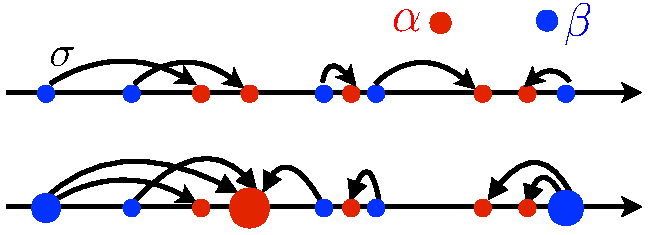
\includegraphics[width=.65\textwidth]{img/1d-schematic}
	\end{center} \pause
	\vspace{-1em}

	This is nice, but somewhat limited. Can we extend this notion to $\mathbb{R}^n$? \pause \newline \\

	\textbf{Idea;} let's \textit{slice and dice}:
	\begin{enumerate}[label=\arabic*.]
		\item Project $n$ features onto $d$ random directions. \pause We now have to solve $d$ 1-D OT problems. \pause
		\item Sort $d$ lists to obtain $d$ optimal transport plans. \pause
		\item Compute the average cost of transportation. \pause
	\end{enumerate}
	
	\textbf{Caveat:} This is is no longer the $p$-Wasserstein Distance.
\end{frame}

\begin{frame}{Sliced Wasserstein Distance ($\nicefrac{3}{4}$)}
	Here's what that looks visually, for a single direction:
	\begin{figure}[h]
		\begin{center}
			\begin{tabular}{@{\hspace{0mm}} c @{}}
				\scalebox{0.93}{
					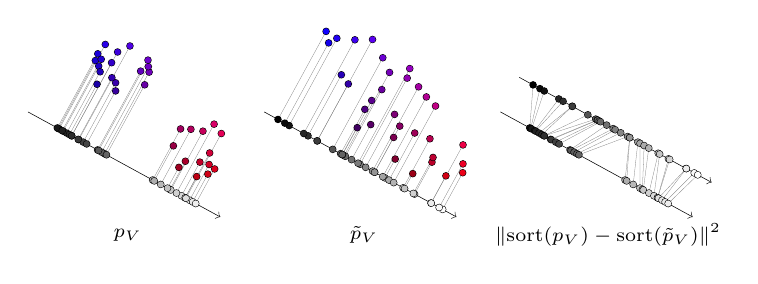
\begin{tikzpicture}
						\begin{scope}[scale=2.0]
							\draw[anchor=center] (0.3, -0.3) node {\scriptsize $p_V$};
							\draw[gray, -, line width = 0.1] (0.7375242851479528,0.07149719324412154) -- (0.6641444194396903,-0.06282374995576157);
\draw[gray, -, line width = 0.1] (0.6352616126167896,0.3741453717776989) -- (0.458051873867213,0.04976512082872764);
\draw[gray, -, line width = 0.1] (0.6659961465969623,0.16905674183969271) -- (0.5680101763503526,-0.01030537359680811);
\draw[gray, -, line width = 0.1] (0.7581160815510639,0.1634410081431301) -- (0.6413191889454982,-0.05035426970552598);
\draw[gray, -, line width = 0.1] (0.8163931968005627,0.14827914918912766) -- (0.6925805086373428,-0.07835845628585919);
\draw[gray, -, line width = 0.1] (0.235522015159636,0.862679580008819) -- (-0.05535171864410808,0.33023878171240917);
\draw[gray, -, line width = 0.1] (0.4358410694203565,0.7349179605485335) -- (0.15267807982339734,0.21659158484790902);
\draw[gray, -, line width = 0.1] (0.09431609762856191,0.808318117172903) -- (-0.14122982199770998,0.3771542033975443);
\draw[gray, -, line width = 0.1] (0.1154706312820831,0.7728239727237151) -- (-0.11000398717238209,0.3600954520850167);
\draw[gray, -, line width = 0.1] (0.3139804373163412,0.9008613797149576) -- (-0.010991312662964757,0.3060045814744292);
\draw[gray, -, line width = 0.1] (0.157427062376505,0.9106254691891364) -- (-0.1356691738613942,0.37411640747552977);
\draw[gray, -, line width = 0.1] (0.8087453710717747,0.0873358066465128) -- (0.7123315540682873,-0.08914850158180204);
\draw[gray, -, line width = 0.1] (0.22286168569889056,0.6672178044029601) -- (0.01713562043085472,0.29063876789360593);
\draw[gray, -, line width = 0.1] (0.22297990357259065,0.6156022713570786) -- (0.03894315277433345,0.27872525867701453);
\draw[gray, -, line width = 0.1] (0.8516233378780766,0.11998168903668985) -- (0.731618788237237,-0.0996851656304995);
\draw[gray, -, line width = 0.1] (0.19926435538276854,0.6994255744573358) -- (-0.014588842711333636,0.307969921097141);
\draw[gray, -, line width = 0.1] (0.38176637786578715,0.7412614969652668) -- (0.10836344286021495,0.24080078135741922);
\draw[gray, -, line width = 0.1] (0.12451618465828287,0.7369979876185243) -- (-0.08796428032668621,0.34805510535978584);
\draw[gray, -, line width = 0.1] (0.10979748007965975,0.8512815509980239) -- (-0.14738305893976042,0.3805157320595852);
\draw[gray, -, line width = 0.1] (0.10479225209789506,0.6579663171400711) -- (-0.06990326093420418,0.3381883254965559);
\draw[gray, -, line width = 0.1] (0.7009834334711795,0.3720120811638443) -- (0.5095651610480088,0.021623283781820712);
\draw[gray, -, line width = 0.1] (0.7773961056233383,0.3599495053784583) -- (0.5734896223674911,-0.013298808598935563);
\draw[gray, -, line width = 0.1] (0.8201340945592945,0.22151647062355037) -- (0.6646480248631804,-0.06309887085251303);
\draw[gray, -, line width = 0.1] (0.131654833648978,0.816398412146849) -- (-0.11587301828711795,0.3633017183959676);
\draw[gray, -, line width = 0.1] (0.6245513907080334,0.13009483281432893) -- (0.5524841077982071,-0.0018234436892857198);
\draw[gray, -, line width = 0.1] (0.430694727643888,0.7696278088773739) -- (0.13411095364295636,0.22673485210952776);
\draw[gray, -, line width = 0.1] (0.1972961888949818,0.7946443747181786) -- (-0.05616655721492772,0.3306839300524687);
\draw[gray, -, line width = 0.1] (0.8941919835488764,0.3450755917066442) -- (0.6696980858024758,-0.06585773171751302);
\draw[gray, -, line width = 0.1] (0.5897943690388352,0.26685768854268516) -- (0.4681749600396796,0.04423485364780588);
\draw[gray, -, line width = 0.1] (0.8482706859776603,0.404644785626021) -- (0.6092688713979999,-0.032845101429043566);
\draw[gray, -, line width = 0.1] (0.4284911662411657,0.8111718300538617) -- (0.11493483408195909,0.23721081397124277);
\draw[gray, -, line width = 0.1] (0.4076415266589243,0.6543043974677796) -- (0.16487715661068447,0.2099271988252185);
\draw[black, ->, line width = 0.2] (-0.3337384061810164,0.4823221222531875) -- (0.8873279753132095,-0.18474948222165583);
\draw[fill={rgb,255:red,0; green,0; blue,0}] (0.7375242851479528,0.07149719324412154) circle (0.020);
\fill[fill={rgb,255:red,188; green,0; blue,18}] (0.7375242851479528,0.07149719324412154) circle (0.020);
\draw[fill={rgb,255:red,0; green,0; blue,0}] (0.6352616126167896,0.3741453717776989) circle (0.020);
\fill[fill={rgb,255:red,161; green,0; blue,95}] (0.6352616126167896,0.3741453717776989) circle (0.020);
\draw[fill={rgb,255:red,0; green,0; blue,0}] (0.6659961465969623,0.16905674183969271) circle (0.020);
\fill[fill={rgb,255:red,169; green,0; blue,43}] (0.6659961465969623,0.16905674183969271) circle (0.020);
\draw[fill={rgb,255:red,0; green,0; blue,0}] (0.7581160815510639,0.1634410081431301) circle (0.020);
\fill[fill={rgb,255:red,193; green,0; blue,41}] (0.7581160815510639,0.1634410081431301) circle (0.020);
\draw[fill={rgb,255:red,0; green,0; blue,0}] (0.8163931968005627,0.14827914918912766) circle (0.020);
\fill[fill={rgb,255:red,208; green,0; blue,37}] (0.8163931968005627,0.14827914918912766) circle (0.020);
\draw[fill={rgb,255:red,0; green,0; blue,0}] (0.235522015159636,0.862679580008819) circle (0.020);
\fill[fill={rgb,255:red,60; green,0; blue,219}] (0.235522015159636,0.862679580008819) circle (0.020);
\draw[fill={rgb,255:red,0; green,0; blue,0}] (0.4358410694203565,0.7349179605485335) circle (0.020);
\fill[fill={rgb,255:red,111; green,0; blue,187}] (0.4358410694203565,0.7349179605485335) circle (0.020);
\draw[fill={rgb,255:red,0; green,0; blue,0}] (0.09431609762856191,0.808318117172903) circle (0.020);
\fill[fill={rgb,255:red,24; green,0; blue,206}] (0.09431609762856191,0.808318117172903) circle (0.020);
\draw[fill={rgb,255:red,0; green,0; blue,0}] (0.1154706312820831,0.7728239727237151) circle (0.020);
\fill[fill={rgb,255:red,29; green,0; blue,197}] (0.1154706312820831,0.7728239727237151) circle (0.020);
\draw[fill={rgb,255:red,0; green,0; blue,0}] (0.3139804373163412,0.9008613797149576) circle (0.020);
\fill[fill={rgb,255:red,80; green,0; blue,229}] (0.3139804373163412,0.9008613797149576) circle (0.020);
\draw[fill={rgb,255:red,0; green,0; blue,0}] (0.157427062376505,0.9106254691891364) circle (0.020);
\fill[fill={rgb,255:red,40; green,0; blue,232}] (0.157427062376505,0.9106254691891364) circle (0.020);
\draw[fill={rgb,255:red,0; green,0; blue,0}] (0.8087453710717747,0.0873358066465128) circle (0.020);
\fill[fill={rgb,255:red,206; green,0; blue,22}] (0.8087453710717747,0.0873358066465128) circle (0.020);
\draw[fill={rgb,255:red,0; green,0; blue,0}] (0.22286168569889056,0.6672178044029601) circle (0.020);
\fill[fill={rgb,255:red,56; green,0; blue,170}] (0.22286168569889056,0.6672178044029601) circle (0.020);
\draw[fill={rgb,255:red,0; green,0; blue,0}] (0.22297990357259065,0.6156022713570786) circle (0.020);
\fill[fill={rgb,255:red,56; green,0; blue,156}] (0.22297990357259065,0.6156022713570786) circle (0.020);
\draw[fill={rgb,255:red,0; green,0; blue,0}] (0.8516233378780766,0.11998168903668985) circle (0.020);
\fill[fill={rgb,255:red,217; green,0; blue,30}] (0.8516233378780766,0.11998168903668985) circle (0.020);
\draw[fill={rgb,255:red,0; green,0; blue,0}] (0.19926435538276854,0.6994255744573358) circle (0.020);
\fill[fill={rgb,255:red,50; green,0; blue,178}] (0.19926435538276854,0.6994255744573358) circle (0.020);
\draw[fill={rgb,255:red,0; green,0; blue,0}] (0.38176637786578715,0.7412614969652668) circle (0.020);
\fill[fill={rgb,255:red,97; green,0; blue,189}] (0.38176637786578715,0.7412614969652668) circle (0.020);
\draw[fill={rgb,255:red,0; green,0; blue,0}] (0.12451618465828287,0.7369979876185243) circle (0.020);
\fill[fill={rgb,255:red,31; green,0; blue,187}] (0.12451618465828287,0.7369979876185243) circle (0.020);
\draw[fill={rgb,255:red,0; green,0; blue,0}] (0.10979748007965975,0.8512815509980239) circle (0.020);
\fill[fill={rgb,255:red,27; green,0; blue,217}] (0.10979748007965975,0.8512815509980239) circle (0.020);
\draw[fill={rgb,255:red,0; green,0; blue,0}] (0.10479225209789506,0.6579663171400711) circle (0.020);
\fill[fill={rgb,255:red,26; green,0; blue,167}] (0.10479225209789506,0.6579663171400711) circle (0.020);
\draw[fill={rgb,255:red,0; green,0; blue,0}] (0.7009834334711795,0.3720120811638443) circle (0.020);
\fill[fill={rgb,255:red,178; green,0; blue,94}] (0.7009834334711795,0.3720120811638443) circle (0.020);
\draw[fill={rgb,255:red,0; green,0; blue,0}] (0.7773961056233383,0.3599495053784583) circle (0.020);
\fill[fill={rgb,255:red,198; green,0; blue,91}] (0.7773961056233383,0.3599495053784583) circle (0.020);
\draw[fill={rgb,255:red,0; green,0; blue,0}] (0.8201340945592945,0.22151647062355037) circle (0.020);
\fill[fill={rgb,255:red,209; green,0; blue,56}] (0.8201340945592945,0.22151647062355037) circle (0.020);
\draw[fill={rgb,255:red,0; green,0; blue,0}] (0.131654833648978,0.816398412146849) circle (0.020);
\fill[fill={rgb,255:red,33; green,0; blue,208}] (0.131654833648978,0.816398412146849) circle (0.020);
\draw[fill={rgb,255:red,0; green,0; blue,0}] (0.6245513907080334,0.13009483281432893) circle (0.020);
\fill[fill={rgb,255:red,159; green,0; blue,33}] (0.6245513907080334,0.13009483281432893) circle (0.020);
\draw[fill={rgb,255:red,0; green,0; blue,0}] (0.430694727643888,0.7696278088773739) circle (0.020);
\fill[fill={rgb,255:red,109; green,0; blue,196}] (0.430694727643888,0.7696278088773739) circle (0.020);
\draw[fill={rgb,255:red,0; green,0; blue,0}] (0.1972961888949818,0.7946443747181786) circle (0.020);
\fill[fill={rgb,255:red,50; green,0; blue,202}] (0.1972961888949818,0.7946443747181786) circle (0.020);
\draw[fill={rgb,255:red,0; green,0; blue,0}] (0.8941919835488764,0.3450755917066442) circle (0.020);
\fill[fill={rgb,255:red,228; green,0; blue,87}] (0.8941919835488764,0.3450755917066442) circle (0.020);
\draw[fill={rgb,255:red,0; green,0; blue,0}] (0.5897943690388352,0.26685768854268516) circle (0.020);
\fill[fill={rgb,255:red,150; green,0; blue,68}] (0.5897943690388352,0.26685768854268516) circle (0.020);
\draw[fill={rgb,255:red,0; green,0; blue,0}] (0.8482706859776603,0.404644785626021) circle (0.020);
\fill[fill={rgb,255:red,216; green,0; blue,103}] (0.8482706859776603,0.404644785626021) circle (0.020);
\draw[fill={rgb,255:red,0; green,0; blue,0}] (0.4284911662411657,0.8111718300538617) circle (0.020);
\fill[fill={rgb,255:red,109; green,0; blue,206}] (0.4284911662411657,0.8111718300538617) circle (0.020);
\draw[fill={rgb,255:red,0; green,0; blue,0}] (0.4076415266589243,0.6543043974677796) circle (0.020);
\fill[fill={rgb,255:red,103; green,0; blue,166}] (0.4076415266589243,0.6543043974677796) circle (0.020);
\draw[fill={rgb,255:red,0; green,0; blue,0}] (0.6641444194396903,-0.06282374995576157) circle (0.020);
\fill[fill={rgb,255:red,221; green,221; blue,221}] (0.6641444194396903,-0.06282374995576157) circle (0.020);
\draw[fill={rgb,255:red,0; green,0; blue,0}] (0.458051873867213,0.04976512082872764) circle (0.020);
\fill[fill={rgb,255:red,171; green,171; blue,171}] (0.458051873867213,0.04976512082872764) circle (0.020);
\draw[fill={rgb,255:red,0; green,0; blue,0}] (0.5680101763503526,-0.01030537359680811) circle (0.020);
\fill[fill={rgb,255:red,198; green,198; blue,198}] (0.5680101763503526,-0.01030537359680811) circle (0.020);
\draw[fill={rgb,255:red,0; green,0; blue,0}] (0.6413191889454982,-0.05035426970552598) circle (0.020);
\fill[fill={rgb,255:red,216; green,216; blue,216}] (0.6413191889454982,-0.05035426970552598) circle (0.020);
\draw[fill={rgb,255:red,0; green,0; blue,0}] (0.6925805086373428,-0.07835845628585919) circle (0.020);
\fill[fill={rgb,255:red,228; green,228; blue,228}] (0.6925805086373428,-0.07835845628585919) circle (0.020);
\draw[fill={rgb,255:red,0; green,0; blue,0}] (-0.05535171864410808,0.33023878171240917) circle (0.020);
\fill[fill={rgb,255:red,46; green,46; blue,46}] (-0.05535171864410808,0.33023878171240917) circle (0.020);
\draw[fill={rgb,255:red,0; green,0; blue,0}] (0.15267807982339734,0.21659158484790902) circle (0.020);
\fill[fill={rgb,255:red,97; green,97; blue,97}] (0.15267807982339734,0.21659158484790902) circle (0.020);
\draw[fill={rgb,255:red,0; green,0; blue,0}] (-0.14122982199770998,0.3771542033975443) circle (0.020);
\fill[fill={rgb,255:red,25; green,25; blue,25}] (-0.14122982199770998,0.3771542033975443) circle (0.020);
\draw[fill={rgb,255:red,0; green,0; blue,0}] (-0.11000398717238209,0.3600954520850167) circle (0.020);
\fill[fill={rgb,255:red,33; green,33; blue,33}] (-0.11000398717238209,0.3600954520850167) circle (0.020);
\draw[fill={rgb,255:red,0; green,0; blue,0}] (-0.010991312662964757,0.3060045814744292) circle (0.020);
\fill[fill={rgb,255:red,57; green,57; blue,57}] (-0.010991312662964757,0.3060045814744292) circle (0.020);
\draw[fill={rgb,255:red,0; green,0; blue,0}] (-0.1356691738613942,0.37411640747552977) circle (0.020);
\fill[fill={rgb,255:red,26; green,26; blue,26}] (-0.1356691738613942,0.37411640747552977) circle (0.020);
\draw[fill={rgb,255:red,0; green,0; blue,0}] (0.7123315540682873,-0.08914850158180204) circle (0.020);
\fill[fill={rgb,255:red,233; green,233; blue,233}] (0.7123315540682873,-0.08914850158180204) circle (0.020);
\draw[fill={rgb,255:red,0; green,0; blue,0}] (0.01713562043085472,0.29063876789360593) circle (0.020);
\fill[fill={rgb,255:red,64; green,64; blue,64}] (0.01713562043085472,0.29063876789360593) circle (0.020);
\draw[fill={rgb,255:red,0; green,0; blue,0}] (0.03894315277433345,0.27872525867701453) circle (0.020);
\fill[fill={rgb,255:red,69; green,69; blue,69}] (0.03894315277433345,0.27872525867701453) circle (0.020);
\draw[fill={rgb,255:red,0; green,0; blue,0}] (0.731618788237237,-0.0996851656304995) circle (0.020);
\fill[fill={rgb,255:red,238; green,238; blue,238}] (0.731618788237237,-0.0996851656304995) circle (0.020);
\draw[fill={rgb,255:red,0; green,0; blue,0}] (-0.014588842711333636,0.307969921097141) circle (0.020);
\fill[fill={rgb,255:red,56; green,56; blue,56}] (-0.014588842711333636,0.307969921097141) circle (0.020);
\draw[fill={rgb,255:red,0; green,0; blue,0}] (0.10836344286021495,0.24080078135741922) circle (0.020);
\fill[fill={rgb,255:red,86; green,86; blue,86}] (0.10836344286021495,0.24080078135741922) circle (0.020);
\draw[fill={rgb,255:red,0; green,0; blue,0}] (-0.08796428032668621,0.34805510535978584) circle (0.020);
\fill[fill={rgb,255:red,38; green,38; blue,38}] (-0.08796428032668621,0.34805510535978584) circle (0.020);
\draw[fill={rgb,255:red,0; green,0; blue,0}] (-0.14738305893976042,0.3805157320595852) circle (0.020);
\fill[fill={rgb,255:red,24; green,24; blue,24}] (-0.14738305893976042,0.3805157320595852) circle (0.020);
\draw[fill={rgb,255:red,0; green,0; blue,0}] (-0.06990326093420418,0.3381883254965559) circle (0.020);
\fill[fill={rgb,255:red,42; green,42; blue,42}] (-0.06990326093420418,0.3381883254965559) circle (0.020);
\draw[fill={rgb,255:red,0; green,0; blue,0}] (0.5095651610480088,0.021623283781820712) circle (0.020);
\fill[fill={rgb,255:red,184; green,184; blue,184}] (0.5095651610480088,0.021623283781820712) circle (0.020);
\draw[fill={rgb,255:red,0; green,0; blue,0}] (0.5734896223674911,-0.013298808598935563) circle (0.020);
\fill[fill={rgb,255:red,199; green,199; blue,199}] (0.5734896223674911,-0.013298808598935563) circle (0.020);
\draw[fill={rgb,255:red,0; green,0; blue,0}] (0.6646480248631804,-0.06309887085251303) circle (0.020);
\fill[fill={rgb,255:red,222; green,222; blue,222}] (0.6646480248631804,-0.06309887085251303) circle (0.020);
\draw[fill={rgb,255:red,0; green,0; blue,0}] (-0.11587301828711795,0.3633017183959676) circle (0.020);
\fill[fill={rgb,255:red,31; green,31; blue,31}] (-0.11587301828711795,0.3633017183959676) circle (0.020);
\draw[fill={rgb,255:red,0; green,0; blue,0}] (0.5524841077982071,-0.0018234436892857198) circle (0.020);
\fill[fill={rgb,255:red,194; green,194; blue,194}] (0.5524841077982071,-0.0018234436892857198) circle (0.020);
\draw[fill={rgb,255:red,0; green,0; blue,0}] (0.13411095364295636,0.22673485210952776) circle (0.020);
\fill[fill={rgb,255:red,92; green,92; blue,92}] (0.13411095364295636,0.22673485210952776) circle (0.020);
\draw[fill={rgb,255:red,0; green,0; blue,0}] (-0.05616655721492772,0.3306839300524687) circle (0.020);
\fill[fill={rgb,255:red,46; green,46; blue,46}] (-0.05616655721492772,0.3306839300524687) circle (0.020);
\draw[fill={rgb,255:red,0; green,0; blue,0}] (0.6696980858024758,-0.06585773171751302) circle (0.020);
\fill[fill={rgb,255:red,223; green,223; blue,223}] (0.6696980858024758,-0.06585773171751302) circle (0.020);
\draw[fill={rgb,255:red,0; green,0; blue,0}] (0.4681749600396796,0.04423485364780588) circle (0.020);
\fill[fill={rgb,255:red,174; green,174; blue,174}] (0.4681749600396796,0.04423485364780588) circle (0.020);
\draw[fill={rgb,255:red,0; green,0; blue,0}] (0.6092688713979999,-0.032845101429043566) circle (0.020);
\fill[fill={rgb,255:red,208; green,208; blue,208}] (0.6092688713979999,-0.032845101429043566) circle (0.020);
\draw[fill={rgb,255:red,0; green,0; blue,0}] (0.11493483408195909,0.23721081397124277) circle (0.020);
\fill[fill={rgb,255:red,88; green,88; blue,88}] (0.11493483408195909,0.23721081397124277) circle (0.020);
\draw[fill={rgb,255:red,0; green,0; blue,0}] (0.16487715661068447,0.2099271988252185) circle (0.020);
\fill[fill={rgb,255:red,100; green,100; blue,100}] (0.16487715661068447,0.2099271988252185) circle (0.020);

						\end{scope}

						\begin{scope}[shift={(3.0,0.0)}, scale=2.0]
							\draw[anchor=center] (0.3, -0.3) node {\scriptsize $\tilde p_V$};
							\draw[gray, -, line width = 0.1] (0.8202041704413296,0.07628025353023737) -- (0.7258080251981646,-0.09651073131436189);
\draw[gray, -, line width = 0.1] (0.4984247674129366,0.18288786191229237) -- (0.43313564235877966,0.0633769201393091);
\draw[gray, -, line width = 0.1] (0.9268010853831867,0.09608852539259066) -- (0.7995697191241723,-0.13680692836123554);
\draw[gray, -, line width = 0.1] (0.5273644078112081,0.39197019254644644) -- (0.36745518244467984,0.0992583189244671);
\draw[gray, -, line width = 0.1] (0.4194488001063227,0.8261326504107683) -- (0.10167629725832766,0.2444539856496782);
\draw[gray, -, line width = 0.1] (0.5743722550301275,0.696873432205544) -- (0.27537471550374976,0.14956210728027605);
\draw[gray, -, line width = 0.1] (0.9289205660903701,0.27286030753684837) -- (0.7268278768308432,-0.09706787880056555);
\draw[gray, -, line width = 0.1] (0.2007151986453794,0.6598150333145507) -- (0.003194086432189271,0.2982550626293187);
\draw[gray, -, line width = 0.1] (0.4622445441871999,0.7329328567767481) -- (0.1738479499694425,0.20502643207745483);
\draw[gray, -, line width = 0.1] (0.342876958634608,0.4017393904958452) -- (0.22126171244982376,0.17912417558156046);
\draw[gray, -, line width = 0.1] (0.3543545048940158,0.9422365848723857) -- (0.0026948047153944822,0.2985278214743372);
\draw[gray, -, line width = 0.1] (0.6466234862868944,0.6416022761181387) -- (0.3542736216292249,0.1064594384179775);
\draw[gray, -, line width = 0.1] (0.15648664390872535,0.7180661420327928) -- (-0.055376894900497985,0.33025253556395995);
\draw[gray, -, line width = 0.1] (0.6223219967194824,0.3482228422560979) -- (0.45899294198800455,0.04925101297122658);
\draw[gray, -, line width = 0.1] (0.48828781340915783,0.32001741705530184) -- (0.36763338463930134,0.09916096662184976);
\draw[gray, -, line width = 0.1] (0.12761947313259792,0.9497758907046843) -- (-0.17509749495794055,0.3956561974609335);
\draw[gray, -, line width = 0.1] (0.7188779739238289,0.31172419194823897) -- (0.5487119167639644,0.00023731366488755068);
\draw[gray, -, line width = 0.1] (0.0756814074676318,0.9205740450269606) -- (-0.20281140319065843,0.41079637453176954);
\draw[gray, -, line width = 0.1] (0.928600733336744,0.1522930123391687) -- (0.7773084975797,-0.12464556760452611);
\draw[gray, -, line width = 0.1] (0.30548567287672435,0.498694337397388) -- (0.15167238328808316,0.21714099936917844);
\draw[gray, -, line width = 0.1] (0.7543365439343221,0.5197342844826867) -- (0.4885031466314675,0.03312951469870301);
\draw[gray, -, line width = 0.1] (0.5906880260232503,0.7574932299904413) -- (0.26243542487465504,0.1566308739677629);
\draw[gray, -, line width = 0.1] (0.7316858778427182,0.1631244864843146) -- (0.6210971089832117,-0.039306897072308666);
\draw[gray, -, line width = 0.1] (0.7384460460186435,0.19313601268748143) -- (0.6136765460430453,-0.03525302506205319);
\draw[gray, -, line width = 0.1] (0.24242220976055634,0.940164811579578) -- (-0.08263831287569709,0.3451455160804835);
\draw[gray, -, line width = 0.1] (0.6097223989603282,0.09038082550318216) -- (0.5577726351282515,-0.004712579337295908);
\draw[gray, -, line width = 0.1] (0.4131667928355628,0.6238257908972612) -- (0.18195587827012355,0.20059705065931785);
\draw[gray, -, line width = 0.1] (0.25715326144486506,0.3821452501067999) -- (0.1634854585301892,0.21068748695170386);
\draw[gray, -, line width = 0.1] (0.6962678910242377,0.5774136803984509) -- (0.41951373760125626,0.07081860062475909);
\draw[gray, -, line width = 0.1] (0.3491204393574636,0.5547379482787673) -- (0.16169821278096097,0.21166386375447);
\draw[gray, -, line width = 0.1] (0.4942989078304718,0.46653182517714653) -- (0.3106190242928545,0.13030805363596473);
\draw[gray, -, line width = 0.1] (0.05955195873105679,0.9936523419991984) -- (-0.24598014999197915,0.43437956839276726);
\draw[black, ->, line width = 0.2] (-0.3337384061810164,0.4823221222531875) -- (0.8873279753132095,-0.18474948222165583);
\draw[fill={rgb,255:red,0; green,0; blue,0}] (0.8202041704413296,0.07628025353023737) circle (0.020);
\fill[fill={rgb,255:red,209; green,0; blue,19}] (0.8202041704413296,0.07628025353023737) circle (0.020);
\draw[fill={rgb,255:red,0; green,0; blue,0}] (0.4984247674129366,0.18288786191229237) circle (0.020);
\fill[fill={rgb,255:red,127; green,0; blue,46}] (0.4984247674129366,0.18288786191229237) circle (0.020);
\draw[fill={rgb,255:red,0; green,0; blue,0}] (0.9268010853831867,0.09608852539259066) circle (0.020);
\fill[fill={rgb,255:red,236; green,0; blue,24}] (0.9268010853831867,0.09608852539259066) circle (0.020);
\draw[fill={rgb,255:red,0; green,0; blue,0}] (0.5273644078112081,0.39197019254644644) circle (0.020);
\fill[fill={rgb,255:red,134; green,0; blue,99}] (0.5273644078112081,0.39197019254644644) circle (0.020);
\draw[fill={rgb,255:red,0; green,0; blue,0}] (0.4194488001063227,0.8261326504107683) circle (0.020);
\fill[fill={rgb,255:red,106; green,0; blue,210}] (0.4194488001063227,0.8261326504107683) circle (0.020);
\draw[fill={rgb,255:red,0; green,0; blue,0}] (0.5743722550301275,0.696873432205544) circle (0.020);
\fill[fill={rgb,255:red,146; green,0; blue,177}] (0.5743722550301275,0.696873432205544) circle (0.020);
\draw[fill={rgb,255:red,0; green,0; blue,0}] (0.9289205660903701,0.27286030753684837) circle (0.020);
\fill[fill={rgb,255:red,236; green,0; blue,69}] (0.9289205660903701,0.27286030753684837) circle (0.020);
\draw[fill={rgb,255:red,0; green,0; blue,0}] (0.2007151986453794,0.6598150333145507) circle (0.020);
\fill[fill={rgb,255:red,51; green,0; blue,168}] (0.2007151986453794,0.6598150333145507) circle (0.020);
\draw[fill={rgb,255:red,0; green,0; blue,0}] (0.4622445441871999,0.7329328567767481) circle (0.020);
\fill[fill={rgb,255:red,117; green,0; blue,186}] (0.4622445441871999,0.7329328567767481) circle (0.020);
\draw[fill={rgb,255:red,0; green,0; blue,0}] (0.342876958634608,0.4017393904958452) circle (0.020);
\fill[fill={rgb,255:red,87; green,0; blue,102}] (0.342876958634608,0.4017393904958452) circle (0.020);
\draw[fill={rgb,255:red,0; green,0; blue,0}] (0.3543545048940158,0.9422365848723857) circle (0.020);
\fill[fill={rgb,255:red,90; green,0; blue,240}] (0.3543545048940158,0.9422365848723857) circle (0.020);
\draw[fill={rgb,255:red,0; green,0; blue,0}] (0.6466234862868944,0.6416022761181387) circle (0.020);
\fill[fill={rgb,255:red,164; green,0; blue,163}] (0.6466234862868944,0.6416022761181387) circle (0.020);
\draw[fill={rgb,255:red,0; green,0; blue,0}] (0.15648664390872535,0.7180661420327928) circle (0.020);
\fill[fill={rgb,255:red,39; green,0; blue,183}] (0.15648664390872535,0.7180661420327928) circle (0.020);
\draw[fill={rgb,255:red,0; green,0; blue,0}] (0.6223219967194824,0.3482228422560979) circle (0.020);
\fill[fill={rgb,255:red,158; green,0; blue,88}] (0.6223219967194824,0.3482228422560979) circle (0.020);
\draw[fill={rgb,255:red,0; green,0; blue,0}] (0.48828781340915783,0.32001741705530184) circle (0.020);
\fill[fill={rgb,255:red,124; green,0; blue,81}] (0.48828781340915783,0.32001741705530184) circle (0.020);
\draw[fill={rgb,255:red,0; green,0; blue,0}] (0.12761947313259792,0.9497758907046843) circle (0.020);
\fill[fill={rgb,255:red,32; green,0; blue,242}] (0.12761947313259792,0.9497758907046843) circle (0.020);
\draw[fill={rgb,255:red,0; green,0; blue,0}] (0.7188779739238289,0.31172419194823897) circle (0.020);
\fill[fill={rgb,255:red,183; green,0; blue,79}] (0.7188779739238289,0.31172419194823897) circle (0.020);
\draw[fill={rgb,255:red,0; green,0; blue,0}] (0.0756814074676318,0.9205740450269606) circle (0.020);
\fill[fill={rgb,255:red,19; green,0; blue,234}] (0.0756814074676318,0.9205740450269606) circle (0.020);
\draw[fill={rgb,255:red,0; green,0; blue,0}] (0.928600733336744,0.1522930123391687) circle (0.020);
\fill[fill={rgb,255:red,236; green,0; blue,38}] (0.928600733336744,0.1522930123391687) circle (0.020);
\draw[fill={rgb,255:red,0; green,0; blue,0}] (0.30548567287672435,0.498694337397388) circle (0.020);
\fill[fill={rgb,255:red,77; green,0; blue,127}] (0.30548567287672435,0.498694337397388) circle (0.020);
\draw[fill={rgb,255:red,0; green,0; blue,0}] (0.7543365439343221,0.5197342844826867) circle (0.020);
\fill[fill={rgb,255:red,192; green,0; blue,132}] (0.7543365439343221,0.5197342844826867) circle (0.020);
\draw[fill={rgb,255:red,0; green,0; blue,0}] (0.5906880260232503,0.7574932299904413) circle (0.020);
\fill[fill={rgb,255:red,150; green,0; blue,193}] (0.5906880260232503,0.7574932299904413) circle (0.020);
\draw[fill={rgb,255:red,0; green,0; blue,0}] (0.7316858778427182,0.1631244864843146) circle (0.020);
\fill[fill={rgb,255:red,186; green,0; blue,41}] (0.7316858778427182,0.1631244864843146) circle (0.020);
\draw[fill={rgb,255:red,0; green,0; blue,0}] (0.7384460460186435,0.19313601268748143) circle (0.020);
\fill[fill={rgb,255:red,188; green,0; blue,49}] (0.7384460460186435,0.19313601268748143) circle (0.020);
\draw[fill={rgb,255:red,0; green,0; blue,0}] (0.24242220976055634,0.940164811579578) circle (0.020);
\fill[fill={rgb,255:red,61; green,0; blue,239}] (0.24242220976055634,0.940164811579578) circle (0.020);
\draw[fill={rgb,255:red,0; green,0; blue,0}] (0.6097223989603282,0.09038082550318216) circle (0.020);
\fill[fill={rgb,255:red,155; green,0; blue,23}] (0.6097223989603282,0.09038082550318216) circle (0.020);
\draw[fill={rgb,255:red,0; green,0; blue,0}] (0.4131667928355628,0.6238257908972612) circle (0.020);
\fill[fill={rgb,255:red,105; green,0; blue,159}] (0.4131667928355628,0.6238257908972612) circle (0.020);
\draw[fill={rgb,255:red,0; green,0; blue,0}] (0.25715326144486506,0.3821452501067999) circle (0.020);
\fill[fill={rgb,255:red,65; green,0; blue,97}] (0.25715326144486506,0.3821452501067999) circle (0.020);
\draw[fill={rgb,255:red,0; green,0; blue,0}] (0.6962678910242377,0.5774136803984509) circle (0.020);
\fill[fill={rgb,255:red,177; green,0; blue,147}] (0.6962678910242377,0.5774136803984509) circle (0.020);
\draw[fill={rgb,255:red,0; green,0; blue,0}] (0.3491204393574636,0.5547379482787673) circle (0.020);
\fill[fill={rgb,255:red,89; green,0; blue,141}] (0.3491204393574636,0.5547379482787673) circle (0.020);
\draw[fill={rgb,255:red,0; green,0; blue,0}] (0.4942989078304718,0.46653182517714653) circle (0.020);
\fill[fill={rgb,255:red,126; green,0; blue,118}] (0.4942989078304718,0.46653182517714653) circle (0.020);
\draw[fill={rgb,255:red,0; green,0; blue,0}] (0.05955195873105679,0.9936523419991984) circle (0.020);
\fill[fill={rgb,255:red,15; green,0; blue,253}] (0.05955195873105679,0.9936523419991984) circle (0.020);
\draw[fill={rgb,255:red,0; green,0; blue,0}] (0.7258080251981646,-0.09651073131436189) circle (0.020);
\fill[fill={rgb,255:red,237; green,237; blue,237}] (0.7258080251981646,-0.09651073131436189) circle (0.020);
\draw[fill={rgb,255:red,0; green,0; blue,0}] (0.43313564235877966,0.0633769201393091) circle (0.020);
\fill[fill={rgb,255:red,165; green,165; blue,165}] (0.43313564235877966,0.0633769201393091) circle (0.020);
\draw[fill={rgb,255:red,0; green,0; blue,0}] (0.7995697191241723,-0.13680692836123554) circle (0.020);
\fill[fill={rgb,255:red,255; green,255; blue,255}] (0.7995697191241723,-0.13680692836123554) circle (0.020);
\draw[fill={rgb,255:red,0; green,0; blue,0}] (0.36745518244467984,0.0992583189244671) circle (0.020);
\fill[fill={rgb,255:red,149; green,149; blue,149}] (0.36745518244467984,0.0992583189244671) circle (0.020);
\draw[fill={rgb,255:red,0; green,0; blue,0}] (0.10167629725832766,0.2444539856496782) circle (0.020);
\fill[fill={rgb,255:red,84; green,84; blue,84}] (0.10167629725832766,0.2444539856496782) circle (0.020);
\draw[fill={rgb,255:red,0; green,0; blue,0}] (0.27537471550374976,0.14956210728027605) circle (0.020);
\fill[fill={rgb,255:red,127; green,127; blue,127}] (0.27537471550374976,0.14956210728027605) circle (0.020);
\draw[fill={rgb,255:red,0; green,0; blue,0}] (0.7268278768308432,-0.09706787880056555) circle (0.020);
\fill[fill={rgb,255:red,237; green,237; blue,237}] (0.7268278768308432,-0.09706787880056555) circle (0.020);
\draw[fill={rgb,255:red,0; green,0; blue,0}] (0.003194086432189271,0.2982550626293187) circle (0.020);
\fill[fill={rgb,255:red,60; green,60; blue,60}] (0.003194086432189271,0.2982550626293187) circle (0.020);
\draw[fill={rgb,255:red,0; green,0; blue,0}] (0.1738479499694425,0.20502643207745483) circle (0.020);
\fill[fill={rgb,255:red,102; green,102; blue,102}] (0.1738479499694425,0.20502643207745483) circle (0.020);
\draw[fill={rgb,255:red,0; green,0; blue,0}] (0.22126171244982376,0.17912417558156046) circle (0.020);
\fill[fill={rgb,255:red,113; green,113; blue,113}] (0.22126171244982376,0.17912417558156046) circle (0.020);
\draw[fill={rgb,255:red,0; green,0; blue,0}] (0.0026948047153944822,0.2985278214743372) circle (0.020);
\fill[fill={rgb,255:red,60; green,60; blue,60}] (0.0026948047153944822,0.2985278214743372) circle (0.020);
\draw[fill={rgb,255:red,0; green,0; blue,0}] (0.3542736216292249,0.1064594384179775) circle (0.020);
\fill[fill={rgb,255:red,146; green,146; blue,146}] (0.3542736216292249,0.1064594384179775) circle (0.020);
\draw[fill={rgb,255:red,0; green,0; blue,0}] (-0.055376894900497985,0.33025253556395995) circle (0.020);
\fill[fill={rgb,255:red,46; green,46; blue,46}] (-0.055376894900497985,0.33025253556395995) circle (0.020);
\draw[fill={rgb,255:red,0; green,0; blue,0}] (0.45899294198800455,0.04925101297122658) circle (0.020);
\fill[fill={rgb,255:red,171; green,171; blue,171}] (0.45899294198800455,0.04925101297122658) circle (0.020);
\draw[fill={rgb,255:red,0; green,0; blue,0}] (0.36763338463930134,0.09916096662184976) circle (0.020);
\fill[fill={rgb,255:red,149; green,149; blue,149}] (0.36763338463930134,0.09916096662184976) circle (0.020);
\draw[fill={rgb,255:red,0; green,0; blue,0}] (-0.17509749495794055,0.3956561974609335) circle (0.020);
\fill[fill={rgb,255:red,17; green,17; blue,17}] (-0.17509749495794055,0.3956561974609335) circle (0.020);
\draw[fill={rgb,255:red,0; green,0; blue,0}] (0.5487119167639644,0.00023731366488755068) circle (0.020);
\fill[fill={rgb,255:red,193; green,193; blue,193}] (0.5487119167639644,0.00023731366488755068) circle (0.020);
\draw[fill={rgb,255:red,0; green,0; blue,0}] (-0.20281140319065843,0.41079637453176954) circle (0.020);
\fill[fill={rgb,255:red,10; green,10; blue,10}] (-0.20281140319065843,0.41079637453176954) circle (0.020);
\draw[fill={rgb,255:red,0; green,0; blue,0}] (0.7773084975797,-0.12464556760452611) circle (0.020);
\fill[fill={rgb,255:red,249; green,249; blue,249}] (0.7773084975797,-0.12464556760452611) circle (0.020);
\draw[fill={rgb,255:red,0; green,0; blue,0}] (0.15167238328808316,0.21714099936917844) circle (0.020);
\fill[fill={rgb,255:red,96; green,96; blue,96}] (0.15167238328808316,0.21714099936917844) circle (0.020);
\draw[fill={rgb,255:red,0; green,0; blue,0}] (0.4885031466314675,0.03312951469870301) circle (0.020);
\fill[fill={rgb,255:red,179; green,179; blue,179}] (0.4885031466314675,0.03312951469870301) circle (0.020);
\draw[fill={rgb,255:red,0; green,0; blue,0}] (0.26243542487465504,0.1566308739677629) circle (0.020);
\fill[fill={rgb,255:red,123; green,123; blue,123}] (0.26243542487465504,0.1566308739677629) circle (0.020);
\draw[fill={rgb,255:red,0; green,0; blue,0}] (0.6210971089832117,-0.039306897072308666) circle (0.020);
\fill[fill={rgb,255:red,211; green,211; blue,211}] (0.6210971089832117,-0.039306897072308666) circle (0.020);
\draw[fill={rgb,255:red,0; green,0; blue,0}] (0.6136765460430453,-0.03525302506205319) circle (0.020);
\fill[fill={rgb,255:red,209; green,209; blue,209}] (0.6136765460430453,-0.03525302506205319) circle (0.020);
\draw[fill={rgb,255:red,0; green,0; blue,0}] (-0.08263831287569709,0.3451455160804835) circle (0.020);
\fill[fill={rgb,255:red,39; green,39; blue,39}] (-0.08263831287569709,0.3451455160804835) circle (0.020);
\draw[fill={rgb,255:red,0; green,0; blue,0}] (0.5577726351282515,-0.004712579337295908) circle (0.020);
\fill[fill={rgb,255:red,196; green,196; blue,196}] (0.5577726351282515,-0.004712579337295908) circle (0.020);
\draw[fill={rgb,255:red,0; green,0; blue,0}] (0.18195587827012355,0.20059705065931785) circle (0.020);
\fill[fill={rgb,255:red,104; green,104; blue,104}] (0.18195587827012355,0.20059705065931785) circle (0.020);
\draw[fill={rgb,255:red,0; green,0; blue,0}] (0.1634854585301892,0.21068748695170386) circle (0.020);
\fill[fill={rgb,255:red,99; green,99; blue,99}] (0.1634854585301892,0.21068748695170386) circle (0.020);
\draw[fill={rgb,255:red,0; green,0; blue,0}] (0.41951373760125626,0.07081860062475909) circle (0.020);
\fill[fill={rgb,255:red,162; green,162; blue,162}] (0.41951373760125626,0.07081860062475909) circle (0.020);
\draw[fill={rgb,255:red,0; green,0; blue,0}] (0.16169821278096097,0.21166386375447) circle (0.020);
\fill[fill={rgb,255:red,99; green,99; blue,99}] (0.16169821278096097,0.21166386375447) circle (0.020);
\draw[fill={rgb,255:red,0; green,0; blue,0}] (0.3106190242928545,0.13030805363596473) circle (0.020);
\fill[fill={rgb,255:red,135; green,135; blue,135}] (0.3106190242928545,0.13030805363596473) circle (0.020);
\draw[fill={rgb,255:red,0; green,0; blue,0}] (-0.24598014999197915,0.43437956839276726) circle (0.020);
\fill[fill={rgb,255:red,0; green,0; blue,0}] (-0.24598014999197915,0.43437956839276726) circle (0.020);

						\end{scope}

						\begin{scope}[shift={(6.0,0.0)}, scale=2.0]
							\draw[anchor=center] (0.35, -0.3) node {\scriptsize ${\|\text{sort}(p_V) - \text{sort}(\tilde p_V )}\|^2$};
							\draw[gray, -, line width = 0.1] (-0.14738305893976042,0.3805157320595852) -- (-0.1261237653409284,0.6537752088653604);
\draw[gray, -, line width = 0.1] (-0.14122982199770998,0.3771542033975443) -- (-0.08295501853960768,0.6301920150043627);
\draw[gray, -, line width = 0.1] (-0.1356691738613942,0.37411640747552977) -- (-0.0552411103068898,0.6150518379335267);
\draw[gray, -, line width = 0.1] (-0.11587301828711795,0.3633017183959676) -- (0.03721807177535366,0.5645411565530767);
\draw[gray, -, line width = 0.1] (-0.11000398717238209,0.3600954520850167) -- (0.06447948975055276,0.5496481760365531);
\draw[gray, -, line width = 0.1] (-0.08796428032668621,0.34805510535978584) -- (0.12255118936644524,0.5179234619469304);
\draw[gray, -, line width = 0.1] (-0.06990326093420418,0.3381883254965559) -- (0.12305047108324002,0.517650703101912);
\draw[gray, -, line width = 0.1] (-0.05616655721492772,0.3306839300524687) -- (0.22153268190937841,0.46384962612227143);
\draw[gray, -, line width = 0.1] (-0.05535171864410808,0.33023878171240917) -- (0.27152876793913394,0.4365366398417716);
\draw[gray, -, line width = 0.1] (-0.014588842711333636,0.307969921097141) -- (0.2815545974320117,0.4310595042270632);
\draw[gray, -, line width = 0.1] (-0.010991312662964757,0.3060045814744292) -- (0.28334184318123995,0.43008312742429705);
\draw[gray, -, line width = 0.1] (0.01713562043085472,0.29063876789360593) -- (0.2937043346204933,0.42442207255004805);
\draw[gray, -, line width = 0.1] (0.03894315277433345,0.27872525867701453) -- (0.3018122629211743,0.41999269113191107);
\draw[gray, -, line width = 0.1] (0.10836344286021495,0.24080078135741922) -- (0.3411180971008745,0.39851981605415365);
\draw[gray, -, line width = 0.1] (0.11493483408195909,0.23721081397124277) -- (0.3822918095257058,0.37602651444035606);
\draw[gray, -, line width = 0.1] (0.13411095364295636,0.22673485210952776) -- (0.3952311001548005,0.36895774775286927);
\draw[gray, -, line width = 0.1] (0.15267807982339734,0.21659158484790902) -- (0.43047540894390524,0.34970369410855795);
\draw[gray, -, line width = 0.1] (0.16487715661068447,0.2099271988252185) -- (0.47413000628027563,0.3258550788905707);
\draw[gray, -, line width = 0.1] (0.458051873867213,0.04976512082872764) -- (0.4873115670957306,0.3186539593970603);
\draw[gray, -, line width = 0.1] (0.4681749600396796,0.04423485364780588) -- (0.4874897692903521,0.31855660709444295);
\draw[gray, -, line width = 0.1] (0.5095651610480088,0.021623283781820712) -- (0.5393701222523071,0.2902142410973523);
\draw[gray, -, line width = 0.1] (0.5524841077982071,-0.0018234436892857198) -- (0.5529920270098304,0.28277256061190226);
\draw[gray, -, line width = 0.1] (0.5680101763503526,-0.01030537359680811) -- (0.5788493266390553,0.26864665344381977);
\draw[gray, -, line width = 0.1] (0.5734896223674911,-0.013298808598935563) -- (0.6083595312825183,0.2525251551712962);
\draw[gray, -, line width = 0.1] (0.6092688713979999,-0.032845101429043566) -- (0.6685683014150151,0.21963295413748074);
\draw[gray, -, line width = 0.1] (0.6413191889454982,-0.05035426970552598) -- (0.6776290197793022,0.21468306113529728);
\draw[gray, -, line width = 0.1] (0.6641444194396903,-0.06282374995576157) -- (0.7335329306940961,0.18414261541054);
\draw[gray, -, line width = 0.1] (0.6646480248631804,-0.06309887085251303) -- (0.7409534936342624,0.18008874340028452);
\draw[gray, -, line width = 0.1] (0.6696980858024758,-0.06585773171751302) -- (0.8456644098492153,0.1228849091582313);
\draw[gray, -, line width = 0.1] (0.6925805086373428,-0.07835845628585919) -- (0.8466842614818939,0.12232776167202764);
\draw[gray, -, line width = 0.1] (0.7123315540682873,-0.08914850158180204) -- (0.8971648822307507,0.09475007286806708);
\draw[gray, -, line width = 0.1] (0.731618788237237,-0.0996851656304995) -- (0.919426103775223,0.08258871211135765);
\draw[black, ->, line width = 0.2] (-0.3337384061810164,0.4823221222531875) -- (0.8873279753132095,-0.18474948222165583);
\draw[black, ->, line width = 0.2] (-0.21388202152996566,0.7017177627257807) -- (1.0071843599642603,0.034646158250937364);
\draw[fill={rgb,255:red,0; green,0; blue,0}] (-0.14738305893976042,0.3805157320595852) circle (0.020);
\fill[fill={rgb,255:red,24; green,24; blue,24}] (-0.14738305893976042,0.3805157320595852) circle (0.020);
\draw[fill={rgb,255:red,0; green,0; blue,0}] (-0.14122982199770998,0.3771542033975443) circle (0.020);
\fill[fill={rgb,255:red,25; green,25; blue,25}] (-0.14122982199770998,0.3771542033975443) circle (0.020);
\draw[fill={rgb,255:red,0; green,0; blue,0}] (-0.1356691738613942,0.37411640747552977) circle (0.020);
\fill[fill={rgb,255:red,26; green,26; blue,26}] (-0.1356691738613942,0.37411640747552977) circle (0.020);
\draw[fill={rgb,255:red,0; green,0; blue,0}] (-0.11587301828711795,0.3633017183959676) circle (0.020);
\fill[fill={rgb,255:red,31; green,31; blue,31}] (-0.11587301828711795,0.3633017183959676) circle (0.020);
\draw[fill={rgb,255:red,0; green,0; blue,0}] (-0.11000398717238209,0.3600954520850167) circle (0.020);
\fill[fill={rgb,255:red,33; green,33; blue,33}] (-0.11000398717238209,0.3600954520850167) circle (0.020);
\draw[fill={rgb,255:red,0; green,0; blue,0}] (-0.08796428032668621,0.34805510535978584) circle (0.020);
\fill[fill={rgb,255:red,38; green,38; blue,38}] (-0.08796428032668621,0.34805510535978584) circle (0.020);
\draw[fill={rgb,255:red,0; green,0; blue,0}] (-0.06990326093420418,0.3381883254965559) circle (0.020);
\fill[fill={rgb,255:red,42; green,42; blue,42}] (-0.06990326093420418,0.3381883254965559) circle (0.020);
\draw[fill={rgb,255:red,0; green,0; blue,0}] (-0.05616655721492772,0.3306839300524687) circle (0.020);
\fill[fill={rgb,255:red,46; green,46; blue,46}] (-0.05616655721492772,0.3306839300524687) circle (0.020);
\draw[fill={rgb,255:red,0; green,0; blue,0}] (-0.05535171864410808,0.33023878171240917) circle (0.020);
\fill[fill={rgb,255:red,46; green,46; blue,46}] (-0.05535171864410808,0.33023878171240917) circle (0.020);
\draw[fill={rgb,255:red,0; green,0; blue,0}] (-0.014588842711333636,0.307969921097141) circle (0.020);
\fill[fill={rgb,255:red,56; green,56; blue,56}] (-0.014588842711333636,0.307969921097141) circle (0.020);
\draw[fill={rgb,255:red,0; green,0; blue,0}] (-0.010991312662964757,0.3060045814744292) circle (0.020);
\fill[fill={rgb,255:red,57; green,57; blue,57}] (-0.010991312662964757,0.3060045814744292) circle (0.020);
\draw[fill={rgb,255:red,0; green,0; blue,0}] (0.01713562043085472,0.29063876789360593) circle (0.020);
\fill[fill={rgb,255:red,64; green,64; blue,64}] (0.01713562043085472,0.29063876789360593) circle (0.020);
\draw[fill={rgb,255:red,0; green,0; blue,0}] (0.03894315277433345,0.27872525867701453) circle (0.020);
\fill[fill={rgb,255:red,69; green,69; blue,69}] (0.03894315277433345,0.27872525867701453) circle (0.020);
\draw[fill={rgb,255:red,0; green,0; blue,0}] (0.10836344286021495,0.24080078135741922) circle (0.020);
\fill[fill={rgb,255:red,86; green,86; blue,86}] (0.10836344286021495,0.24080078135741922) circle (0.020);
\draw[fill={rgb,255:red,0; green,0; blue,0}] (0.11493483408195909,0.23721081397124277) circle (0.020);
\fill[fill={rgb,255:red,88; green,88; blue,88}] (0.11493483408195909,0.23721081397124277) circle (0.020);
\draw[fill={rgb,255:red,0; green,0; blue,0}] (0.13411095364295636,0.22673485210952776) circle (0.020);
\fill[fill={rgb,255:red,92; green,92; blue,92}] (0.13411095364295636,0.22673485210952776) circle (0.020);
\draw[fill={rgb,255:red,0; green,0; blue,0}] (0.15267807982339734,0.21659158484790902) circle (0.020);
\fill[fill={rgb,255:red,97; green,97; blue,97}] (0.15267807982339734,0.21659158484790902) circle (0.020);
\draw[fill={rgb,255:red,0; green,0; blue,0}] (0.16487715661068447,0.2099271988252185) circle (0.020);
\fill[fill={rgb,255:red,100; green,100; blue,100}] (0.16487715661068447,0.2099271988252185) circle (0.020);
\draw[fill={rgb,255:red,0; green,0; blue,0}] (0.458051873867213,0.04976512082872764) circle (0.020);
\fill[fill={rgb,255:red,171; green,171; blue,171}] (0.458051873867213,0.04976512082872764) circle (0.020);
\draw[fill={rgb,255:red,0; green,0; blue,0}] (0.4681749600396796,0.04423485364780588) circle (0.020);
\fill[fill={rgb,255:red,174; green,174; blue,174}] (0.4681749600396796,0.04423485364780588) circle (0.020);
\draw[fill={rgb,255:red,0; green,0; blue,0}] (0.5095651610480088,0.021623283781820712) circle (0.020);
\fill[fill={rgb,255:red,184; green,184; blue,184}] (0.5095651610480088,0.021623283781820712) circle (0.020);
\draw[fill={rgb,255:red,0; green,0; blue,0}] (0.5524841077982071,-0.0018234436892857198) circle (0.020);
\fill[fill={rgb,255:red,194; green,194; blue,194}] (0.5524841077982071,-0.0018234436892857198) circle (0.020);
\draw[fill={rgb,255:red,0; green,0; blue,0}] (0.5680101763503526,-0.01030537359680811) circle (0.020);
\fill[fill={rgb,255:red,198; green,198; blue,198}] (0.5680101763503526,-0.01030537359680811) circle (0.020);
\draw[fill={rgb,255:red,0; green,0; blue,0}] (0.5734896223674911,-0.013298808598935563) circle (0.020);
\fill[fill={rgb,255:red,199; green,199; blue,199}] (0.5734896223674911,-0.013298808598935563) circle (0.020);
\draw[fill={rgb,255:red,0; green,0; blue,0}] (0.6092688713979999,-0.032845101429043566) circle (0.020);
\fill[fill={rgb,255:red,208; green,208; blue,208}] (0.6092688713979999,-0.032845101429043566) circle (0.020);
\draw[fill={rgb,255:red,0; green,0; blue,0}] (0.6413191889454982,-0.05035426970552598) circle (0.020);
\fill[fill={rgb,255:red,216; green,216; blue,216}] (0.6413191889454982,-0.05035426970552598) circle (0.020);
\draw[fill={rgb,255:red,0; green,0; blue,0}] (0.6641444194396903,-0.06282374995576157) circle (0.020);
\fill[fill={rgb,255:red,221; green,221; blue,221}] (0.6641444194396903,-0.06282374995576157) circle (0.020);
\draw[fill={rgb,255:red,0; green,0; blue,0}] (0.6646480248631804,-0.06309887085251303) circle (0.020);
\fill[fill={rgb,255:red,222; green,222; blue,222}] (0.6646480248631804,-0.06309887085251303) circle (0.020);
\draw[fill={rgb,255:red,0; green,0; blue,0}] (0.6696980858024758,-0.06585773171751302) circle (0.020);
\fill[fill={rgb,255:red,223; green,223; blue,223}] (0.6696980858024758,-0.06585773171751302) circle (0.020);
\draw[fill={rgb,255:red,0; green,0; blue,0}] (0.6925805086373428,-0.07835845628585919) circle (0.020);
\fill[fill={rgb,255:red,228; green,228; blue,228}] (0.6925805086373428,-0.07835845628585919) circle (0.020);
\draw[fill={rgb,255:red,0; green,0; blue,0}] (0.7123315540682873,-0.08914850158180204) circle (0.020);
\fill[fill={rgb,255:red,233; green,233; blue,233}] (0.7123315540682873,-0.08914850158180204) circle (0.020);
\draw[fill={rgb,255:red,0; green,0; blue,0}] (0.731618788237237,-0.0996851656304995) circle (0.020);
\fill[fill={rgb,255:red,238; green,238; blue,238}] (0.731618788237237,-0.0996851656304995) circle (0.020);
\draw[fill={rgb,255:red,0; green,0; blue,0}] (-0.1261237653409284,0.6537752088653604) circle (0.020);
\fill[fill={rgb,255:red,0; green,0; blue,0}] (-0.1261237653409284,0.6537752088653604) circle (0.020);
\draw[fill={rgb,255:red,0; green,0; blue,0}] (-0.08295501853960768,0.6301920150043627) circle (0.020);
\fill[fill={rgb,255:red,10; green,10; blue,10}] (-0.08295501853960768,0.6301920150043627) circle (0.020);
\draw[fill={rgb,255:red,0; green,0; blue,0}] (-0.0552411103068898,0.6150518379335267) circle (0.020);
\fill[fill={rgb,255:red,17; green,17; blue,17}] (-0.0552411103068898,0.6150518379335267) circle (0.020);
\draw[fill={rgb,255:red,0; green,0; blue,0}] (0.03721807177535366,0.5645411565530767) circle (0.020);
\fill[fill={rgb,255:red,39; green,39; blue,39}] (0.03721807177535366,0.5645411565530767) circle (0.020);
\draw[fill={rgb,255:red,0; green,0; blue,0}] (0.06447948975055276,0.5496481760365531) circle (0.020);
\fill[fill={rgb,255:red,46; green,46; blue,46}] (0.06447948975055276,0.5496481760365531) circle (0.020);
\draw[fill={rgb,255:red,0; green,0; blue,0}] (0.12255118936644524,0.5179234619469304) circle (0.020);
\fill[fill={rgb,255:red,60; green,60; blue,60}] (0.12255118936644524,0.5179234619469304) circle (0.020);
\draw[fill={rgb,255:red,0; green,0; blue,0}] (0.12305047108324002,0.517650703101912) circle (0.020);
\fill[fill={rgb,255:red,60; green,60; blue,60}] (0.12305047108324002,0.517650703101912) circle (0.020);
\draw[fill={rgb,255:red,0; green,0; blue,0}] (0.22153268190937841,0.46384962612227143) circle (0.020);
\fill[fill={rgb,255:red,84; green,84; blue,84}] (0.22153268190937841,0.46384962612227143) circle (0.020);
\draw[fill={rgb,255:red,0; green,0; blue,0}] (0.27152876793913394,0.4365366398417716) circle (0.020);
\fill[fill={rgb,255:red,96; green,96; blue,96}] (0.27152876793913394,0.4365366398417716) circle (0.020);
\draw[fill={rgb,255:red,0; green,0; blue,0}] (0.2815545974320117,0.4310595042270632) circle (0.020);
\fill[fill={rgb,255:red,99; green,99; blue,99}] (0.2815545974320117,0.4310595042270632) circle (0.020);
\draw[fill={rgb,255:red,0; green,0; blue,0}] (0.28334184318123995,0.43008312742429705) circle (0.020);
\fill[fill={rgb,255:red,99; green,99; blue,99}] (0.28334184318123995,0.43008312742429705) circle (0.020);
\draw[fill={rgb,255:red,0; green,0; blue,0}] (0.2937043346204933,0.42442207255004805) circle (0.020);
\fill[fill={rgb,255:red,102; green,102; blue,102}] (0.2937043346204933,0.42442207255004805) circle (0.020);
\draw[fill={rgb,255:red,0; green,0; blue,0}] (0.3018122629211743,0.41999269113191107) circle (0.020);
\fill[fill={rgb,255:red,104; green,104; blue,104}] (0.3018122629211743,0.41999269113191107) circle (0.020);
\draw[fill={rgb,255:red,0; green,0; blue,0}] (0.3411180971008745,0.39851981605415365) circle (0.020);
\fill[fill={rgb,255:red,113; green,113; blue,113}] (0.3411180971008745,0.39851981605415365) circle (0.020);
\draw[fill={rgb,255:red,0; green,0; blue,0}] (0.3822918095257058,0.37602651444035606) circle (0.020);
\fill[fill={rgb,255:red,123; green,123; blue,123}] (0.3822918095257058,0.37602651444035606) circle (0.020);
\draw[fill={rgb,255:red,0; green,0; blue,0}] (0.3952311001548005,0.36895774775286927) circle (0.020);
\fill[fill={rgb,255:red,127; green,127; blue,127}] (0.3952311001548005,0.36895774775286927) circle (0.020);
\draw[fill={rgb,255:red,0; green,0; blue,0}] (0.43047540894390524,0.34970369410855795) circle (0.020);
\fill[fill={rgb,255:red,135; green,135; blue,135}] (0.43047540894390524,0.34970369410855795) circle (0.020);
\draw[fill={rgb,255:red,0; green,0; blue,0}] (0.47413000628027563,0.3258550788905707) circle (0.020);
\fill[fill={rgb,255:red,146; green,146; blue,146}] (0.47413000628027563,0.3258550788905707) circle (0.020);
\draw[fill={rgb,255:red,0; green,0; blue,0}] (0.4873115670957306,0.3186539593970603) circle (0.020);
\fill[fill={rgb,255:red,149; green,149; blue,149}] (0.4873115670957306,0.3186539593970603) circle (0.020);
\draw[fill={rgb,255:red,0; green,0; blue,0}] (0.4874897692903521,0.31855660709444295) circle (0.020);
\fill[fill={rgb,255:red,149; green,149; blue,149}] (0.4874897692903521,0.31855660709444295) circle (0.020);
\draw[fill={rgb,255:red,0; green,0; blue,0}] (0.5393701222523071,0.2902142410973523) circle (0.020);
\fill[fill={rgb,255:red,162; green,162; blue,162}] (0.5393701222523071,0.2902142410973523) circle (0.020);
\draw[fill={rgb,255:red,0; green,0; blue,0}] (0.5529920270098304,0.28277256061190226) circle (0.020);
\fill[fill={rgb,255:red,165; green,165; blue,165}] (0.5529920270098304,0.28277256061190226) circle (0.020);
\draw[fill={rgb,255:red,0; green,0; blue,0}] (0.5788493266390553,0.26864665344381977) circle (0.020);
\fill[fill={rgb,255:red,171; green,171; blue,171}] (0.5788493266390553,0.26864665344381977) circle (0.020);
\draw[fill={rgb,255:red,0; green,0; blue,0}] (0.6083595312825183,0.2525251551712962) circle (0.020);
\fill[fill={rgb,255:red,179; green,179; blue,179}] (0.6083595312825183,0.2525251551712962) circle (0.020);
\draw[fill={rgb,255:red,0; green,0; blue,0}] (0.6685683014150151,0.21963295413748074) circle (0.020);
\fill[fill={rgb,255:red,193; green,193; blue,193}] (0.6685683014150151,0.21963295413748074) circle (0.020);
\draw[fill={rgb,255:red,0; green,0; blue,0}] (0.6776290197793022,0.21468306113529728) circle (0.020);
\fill[fill={rgb,255:red,196; green,196; blue,196}] (0.6776290197793022,0.21468306113529728) circle (0.020);
\draw[fill={rgb,255:red,0; green,0; blue,0}] (0.7335329306940961,0.18414261541054) circle (0.020);
\fill[fill={rgb,255:red,209; green,209; blue,209}] (0.7335329306940961,0.18414261541054) circle (0.020);
\draw[fill={rgb,255:red,0; green,0; blue,0}] (0.7409534936342624,0.18008874340028452) circle (0.020);
\fill[fill={rgb,255:red,211; green,211; blue,211}] (0.7409534936342624,0.18008874340028452) circle (0.020);
\draw[fill={rgb,255:red,0; green,0; blue,0}] (0.8456644098492153,0.1228849091582313) circle (0.020);
\fill[fill={rgb,255:red,237; green,237; blue,237}] (0.8456644098492153,0.1228849091582313) circle (0.020);
\draw[fill={rgb,255:red,0; green,0; blue,0}] (0.8466842614818939,0.12232776167202764) circle (0.020);
\fill[fill={rgb,255:red,237; green,237; blue,237}] (0.8466842614818939,0.12232776167202764) circle (0.020);
\draw[fill={rgb,255:red,0; green,0; blue,0}] (0.8971648822307507,0.09475007286806708) circle (0.020);
\fill[fill={rgb,255:red,249; green,249; blue,249}] (0.8971648822307507,0.09475007286806708) circle (0.020);
\draw[fill={rgb,255:red,0; green,0; blue,0}] (0.919426103775223,0.08258871211135765) circle (0.020);
\fill[fill={rgb,255:red,255; green,255; blue,255}] (0.919426103775223,0.08258871211135765) circle (0.020);

						\end{scope}
					\end{tikzpicture}
				}
			\end{tabular}
		\end{center}
	\end{figure} \pause

	Crucially, Sliced Wasserstein Distance is \textbf{differentiable}, which enables us to use optimize transport cost using neural nets. E.g.~texture matching:
	\vspace{-1em}
	\begin{figure}[h]
		\hspace{-1em}
		\centering
		\begin{tabular}{@{} c @{\hspace{0.5mm}} c @{\hspace{1mm}} c @{\hspace{0.5mm}} c @{\hspace{1mm}} c @{\hspace{0.5mm}} c @{}}
			{\scriptsize\textbf{input}} & {\scriptsize\textbf{generated}} &
			{\scriptsize\textbf{input}} & {\scriptsize\textbf{generated}} \\
			\fbox{
\includegraphics[height=1.6cm]{img/generative/input/leopard1_256.jpg}} &
			\fbox{
\includegraphics[height=1.6cm, trim=1415 0 0 0, clip]{img/generative/banner/leopard1_synth1x8leopard1_arch-TextureNetV1_loss-VGGnormalized-Slicing_rotation-random_always_LR-1_00e-03_B-8.jpg}} &
			\fbox{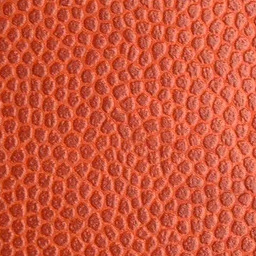
\includegraphics[height=1.6cm]{img/generative/input/skin256.jpg}} &
			\fbox{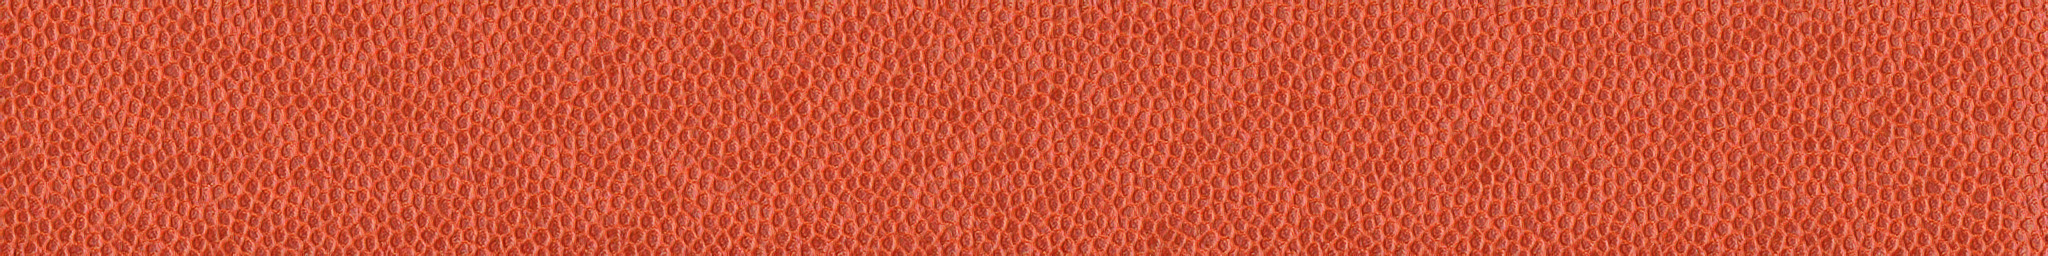
\includegraphics[height=1.6cm, trim=1415 0 0 0, clip]{img/generative/banner/skin_synth1x8skin_arch-TextureNetV1_loss-VGGnormalized-Slicing_rotation-random_always_LR-1_00e-03_B-8.jpg}}
		\end{tabular}
	\end{figure}



\end{frame}

\begin{frame}{Sliced Wasserstein Distance ($\nicefrac{4}{4}$)}
	\textbf{Spatial Priors:} Projections act on point clouds, which rids spatial information in learning the input distribution. \pause \newline \\

	A trick to recover spatial structure is to cluster-sort by spatial dimension:
	\setlength{\fboxsep}{0pt}\setlength{\fboxrule}{0.8pt}
	\begin{figure}[!h]
		\begin{center}
			\hspace{-15mm}
			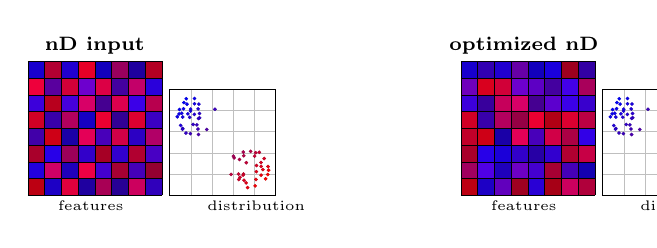
\begin{tikzpicture}
				% Target
				\begin{scope}
					\draw (0.85, 1.4) node[anchor=center] {\scriptsize \textbf{nD input}};
					\begin{scope}[shift={(0.0,-0.5)}, scale=1.7]
						\fill[fill={rgb,255:red,188; green,0; blue,18}]  (0.0,0.0) -- (0.125,0.0) -- (0.125,0.125) -- (0.0,0.125);
\fill[fill={rgb,255:red,34; green,0; blue,222}]  (0.0,0.125) -- (0.125,0.125) -- (0.125,0.25) -- (0.0,0.25);
\fill[fill={rgb,255:red,169; green,0; blue,43}]  (0.0,0.25) -- (0.125,0.25) -- (0.125,0.375) -- (0.0,0.375);
\fill[fill={rgb,255:red,65; green,0; blue,169}]  (0.0,0.375) -- (0.125,0.375) -- (0.125,0.5) -- (0.0,0.5);
\fill[fill={rgb,255:red,208; green,0; blue,37}]  (0.0,0.5) -- (0.125,0.5) -- (0.125,0.625) -- (0.0,0.625);
\fill[fill={rgb,255:red,60; green,0; blue,219}]  (0.0,0.625) -- (0.125,0.625) -- (0.125,0.75) -- (0.0,0.75);
\fill[fill={rgb,255:red,238; green,0; blue,59}]  (0.0,0.75) -- (0.125,0.75) -- (0.125,0.875) -- (0.0,0.875);
\fill[fill={rgb,255:red,24; green,0; blue,206}]  (0.0,0.875) -- (0.125,0.875) -- (0.125,1.0) -- (0.0,1.0);
\fill[fill={rgb,255:red,29; green,0; blue,197}]  (0.125,0.0) -- (0.25,0.0) -- (0.25,0.125) -- (0.125,0.125);
\fill[fill={rgb,255:red,207; green,0; blue,102}]  (0.125,0.125) -- (0.25,0.125) -- (0.25,0.25) -- (0.125,0.25);
\fill[fill={rgb,255:red,40; green,0; blue,232}]  (0.125,0.25) -- (0.25,0.25) -- (0.25,0.375) -- (0.125,0.375);
\fill[fill={rgb,255:red,206; green,0; blue,22}]  (0.125,0.375) -- (0.25,0.375) -- (0.25,0.5) -- (0.125,0.5);
\fill[fill={rgb,255:red,56; green,0; blue,170}]  (0.125,0.5) -- (0.25,0.5) -- (0.25,0.625) -- (0.125,0.625);
\fill[fill={rgb,255:red,184; green,0; blue,29}]  (0.125,0.625) -- (0.25,0.625) -- (0.25,0.75) -- (0.125,0.75);
\fill[fill={rgb,255:red,89; green,0; blue,158}]  (0.125,0.75) -- (0.25,0.75) -- (0.25,0.875) -- (0.125,0.875);
\fill[fill={rgb,255:red,178; green,0; blue,50}]  (0.125,0.875) -- (0.25,0.875) -- (0.25,1.0) -- (0.125,1.0);
\fill[fill={rgb,255:red,224; green,0; blue,61}]  (0.25,0.0) -- (0.375,0.0) -- (0.375,0.125) -- (0.25,0.125);
\fill[fill={rgb,255:red,31; green,0; blue,187}]  (0.25,0.125) -- (0.375,0.125) -- (0.375,0.25) -- (0.25,0.25);
\fill[fill={rgb,255:red,155; green,0; blue,89}]  (0.25,0.25) -- (0.375,0.25) -- (0.375,0.375) -- (0.25,0.375);
\fill[fill={rgb,255:red,26; green,0; blue,167}]  (0.25,0.375) -- (0.375,0.375) -- (0.375,0.5) -- (0.25,0.5);
\fill[fill={rgb,255:red,178; green,0; blue,94}]  (0.25,0.5) -- (0.375,0.5) -- (0.375,0.625) -- (0.25,0.625);
\fill[fill={rgb,255:red,70; green,0; blue,219}]  (0.25,0.625) -- (0.375,0.625) -- (0.375,0.75) -- (0.25,0.75);
\fill[fill={rgb,255:red,209; green,0; blue,56}]  (0.25,0.75) -- (0.375,0.75) -- (0.375,0.875) -- (0.25,0.875);
\fill[fill={rgb,255:red,33; green,0; blue,208}]  (0.25,0.875) -- (0.375,0.875) -- (0.375,1.0) -- (0.25,1.0);
\fill[fill={rgb,255:red,31; green,0; blue,160}]  (0.375,0.0) -- (0.5,0.0) -- (0.5,0.125) -- (0.375,0.125);
\fill[fill={rgb,255:red,237; green,0; blue,68}]  (0.375,0.125) -- (0.5,0.125) -- (0.5,0.25) -- (0.375,0.25);
\fill[fill={rgb,255:red,50; green,0; blue,202}]  (0.375,0.25) -- (0.5,0.25) -- (0.5,0.375) -- (0.375,0.375);
\fill[fill={rgb,255:red,228; green,0; blue,87}]  (0.375,0.375) -- (0.5,0.375) -- (0.5,0.5) -- (0.375,0.5);
\fill[fill={rgb,255:red,22; green,0; blue,195}]  (0.375,0.5) -- (0.5,0.5) -- (0.5,0.625) -- (0.375,0.625);
\fill[fill={rgb,255:red,216; green,0; blue,103}]  (0.375,0.625) -- (0.5,0.625) -- (0.5,0.75) -- (0.375,0.75);
\fill[fill={rgb,255:red,109; green,0; blue,206}]  (0.375,0.75) -- (0.5,0.75) -- (0.5,0.875) -- (0.375,0.875);
\fill[fill={rgb,255:red,231; green,0; blue,39}]  (0.375,0.875) -- (0.5,0.875) -- (0.5,1.0) -- (0.375,1.0);
\fill[fill={rgb,255:red,168; green,0; blue,85}]  (0.5,0.0) -- (0.625,0.0) -- (0.625,0.125) -- (0.5,0.125);
\fill[fill={rgb,255:red,68; green,0; blue,207}]  (0.5,0.125) -- (0.625,0.125) -- (0.625,0.25) -- (0.5,0.25);
\fill[fill={rgb,255:red,166; green,0; blue,37}]  (0.5,0.25) -- (0.625,0.25) -- (0.625,0.375) -- (0.5,0.375);
\fill[fill={rgb,255:red,72; green,0; blue,186}]  (0.5,0.375) -- (0.625,0.375) -- (0.625,0.5) -- (0.5,0.5);
\fill[fill={rgb,255:red,236; green,0; blue,49}]  (0.5,0.5) -- (0.625,0.5) -- (0.625,0.625) -- (0.5,0.625);
\fill[fill={rgb,255:red,69; green,0; blue,145}]  (0.5,0.625) -- (0.625,0.625) -- (0.625,0.75) -- (0.5,0.75);
\fill[fill={rgb,255:red,220; green,0; blue,69}]  (0.5,0.75) -- (0.625,0.75) -- (0.625,0.875) -- (0.5,0.875);
\fill[fill={rgb,255:red,18; green,0; blue,188}]  (0.5,0.875) -- (0.625,0.875) -- (0.625,1.0) -- (0.5,1.0);
\fill[fill={rgb,255:red,39; green,0; blue,149}]  (0.625,0.0) -- (0.75,0.0) -- (0.75,0.125) -- (0.625,0.125);
\fill[fill={rgb,255:red,166; green,0; blue,51}]  (0.625,0.125) -- (0.75,0.125) -- (0.75,0.25) -- (0.625,0.25);
\fill[fill={rgb,255:red,50; green,0; blue,207}]  (0.625,0.25) -- (0.75,0.25) -- (0.75,0.375) -- (0.625,0.375);
\fill[fill={rgb,255:red,209; green,0; blue,71}]  (0.625,0.375) -- (0.75,0.375) -- (0.75,0.5) -- (0.625,0.5);
\fill[fill={rgb,255:red,50; green,0; blue,148}]  (0.625,0.5) -- (0.75,0.5) -- (0.75,0.625) -- (0.625,0.625);
\fill[fill={rgb,255:red,220; green,0; blue,78}]  (0.625,0.625) -- (0.75,0.625) -- (0.75,0.75) -- (0.625,0.75);
\fill[fill={rgb,255:red,68; green,0; blue,159}]  (0.625,0.75) -- (0.75,0.75) -- (0.75,0.875) -- (0.625,0.875);
\fill[fill={rgb,255:red,153; green,0; blue,93}]  (0.625,0.875) -- (0.75,0.875) -- (0.75,1.0) -- (0.625,1.0);
\fill[fill={rgb,255:red,204; green,0; blue,94}]  (0.75,0.0) -- (0.875,0.0) -- (0.875,0.125) -- (0.75,0.125);
\fill[fill={rgb,255:red,69; green,0; blue,184}]  (0.75,0.125) -- (0.875,0.125) -- (0.875,0.25) -- (0.75,0.25);
\fill[fill={rgb,255:red,177; green,0; blue,48}]  (0.75,0.25) -- (0.875,0.25) -- (0.875,0.375) -- (0.75,0.375);
\fill[fill={rgb,255:red,44; green,0; blue,195}]  (0.75,0.375) -- (0.875,0.375) -- (0.875,0.5) -- (0.75,0.5);
\fill[fill={rgb,255:red,220; green,0; blue,48}]  (0.75,0.5) -- (0.875,0.5) -- (0.875,0.625) -- (0.75,0.625);
\fill[fill={rgb,255:red,59; green,0; blue,232}]  (0.75,0.625) -- (0.875,0.625) -- (0.875,0.75) -- (0.75,0.75);
\fill[fill={rgb,255:red,195; green,0; blue,105}]  (0.75,0.75) -- (0.875,0.75) -- (0.875,0.875) -- (0.75,0.875);
\fill[fill={rgb,255:red,31; green,0; blue,158}]  (0.75,0.875) -- (0.875,0.875) -- (0.875,1.0) -- (0.75,1.0);
\fill[fill={rgb,255:red,48; green,0; blue,187}]  (0.875,0.0) -- (1.0,0.0) -- (1.0,0.125) -- (0.875,0.125);
\fill[fill={rgb,255:red,148; green,0; blue,49}]  (0.875,0.125) -- (1.0,0.125) -- (1.0,0.25) -- (0.875,0.25);
\fill[fill={rgb,255:red,72; green,0; blue,196}]  (0.875,0.25) -- (1.0,0.25) -- (1.0,0.375) -- (0.875,0.375);
\fill[fill={rgb,255:red,177; green,0; blue,103}]  (0.875,0.375) -- (1.0,0.375) -- (1.0,0.5) -- (0.875,0.5);
\fill[fill={rgb,255:red,59; green,0; blue,194}]  (0.875,0.5) -- (1.0,0.5) -- (1.0,0.625) -- (0.875,0.625);
\fill[fill={rgb,255:red,184; green,0; blue,78}]  (0.875,0.625) -- (1.0,0.625) -- (1.0,0.75) -- (0.875,0.75);
\fill[fill={rgb,255:red,42; green,0; blue,219}]  (0.875,0.75) -- (1.0,0.75) -- (1.0,0.875) -- (0.875,0.875);
\fill[fill={rgb,255:red,179; green,0; blue,35}]  (0.875,0.875) -- (1.0,0.875) -- (1.0,1.0) -- (0.875,1.0);
\draw[black, -, line width = 0.1] (0,0.0) -- (1,0.0);
\draw[black, -, line width = 0.1] (0.0, 0) -- (0.0, 1);
\draw[black, -, line width = 0.1] (0,0.125) -- (1,0.125);
\draw[black, -, line width = 0.1] (0.125, 0) -- (0.125, 1);
\draw[black, -, line width = 0.1] (0,0.25) -- (1,0.25);
\draw[black, -, line width = 0.1] (0.25, 0) -- (0.25, 1);
\draw[black, -, line width = 0.1] (0,0.375) -- (1,0.375);
\draw[black, -, line width = 0.1] (0.375, 0) -- (0.375, 1);
\draw[black, -, line width = 0.1] (0,0.5) -- (1,0.5);
\draw[black, -, line width = 0.1] (0.5, 0) -- (0.5, 1);
\draw[black, -, line width = 0.1] (0,0.625) -- (1,0.625);
\draw[black, -, line width = 0.1] (0.625, 0) -- (0.625, 1);
\draw[black, -, line width = 0.1] (0,0.75) -- (1,0.75);
\draw[black, -, line width = 0.1] (0.75, 0) -- (0.75, 1);
\draw[black, -, line width = 0.1] (0,0.875) -- (1,0.875);
\draw[black, -, line width = 0.1] (0.875, 0) -- (0.875, 1);
\draw[black, -, line width = 0.1] (0,1.0) -- (1,1.0);
\draw[black, -, line width = 0.1] (1.0, 0) -- (1.0, 1);
					\end{scope}

					% Plots
					\begin{scope}[shift={(1.8,-0.5)}, scale=0.3]
						\begin{axis}[width=0.5\textwidth,height=0.5\textwidth,grid=major,xmin=0.0,xmax=1.0,ymin=0.0,ymax=1.0,ticks=none]
	\addplot[only marks, scatter,colormap name=mine,point meta=y-x,domain=0:1] 
		coordinates {
( 0.7375242851479528 , 0.07149719324412154 )
( 0.1352616126167896 , 0.8741453717776989 )
( 0.6659961465969623 , 0.16905674183969271 )
( 0.25811608155106386 , 0.6634410081431301 )
( 0.8163931968005627 , 0.14827914918912766 )
( 0.235522015159636 , 0.862679580008819 )
( 0.9358410694203565 , 0.23491796054853353 )
( 0.09431609762856191 , 0.808318117172903 )
( 0.1154706312820831 , 0.7728239727237151 )
( 0.8139804373163412 , 0.4008613797149576 )
( 0.157427062376505 , 0.9106254691891366 )
( 0.8087453710717747 , 0.0873358066465128 )
( 0.22286168569889056 , 0.6672178044029601 )
( 0.7229799035725907 , 0.11560227135707851 )
( 0.35162333787807665 , 0.6199816890366898 )
( 0.6992643553827685 , 0.19942557445733575 )
( 0.8817663778657872 , 0.2412614969652668 )
( 0.12451618465828287 , 0.7369979876185243 )
( 0.6097974800796597 , 0.35128155099802394 )
( 0.10479225209789506 , 0.6579663171400711 )
( 0.7009834334711795 , 0.3720120811638443 )
( 0.27739610562333833 , 0.8599495053784584 )
( 0.8201340945592945 , 0.22151647062355037 )
( 0.131654833648978 , 0.816398412146849 )
( 0.1245513907080335 , 0.630094832814329 )
( 0.9306947276438879 , 0.26962780887737386 )
( 0.1972961888949818 , 0.7946443747181786 )
( 0.8941919835488764 , 0.3450755917066442 )
( 0.08979436903883525 , 0.7668576885426852 )
( 0.8482706859776603 , 0.404644785626021 )
( 0.4284911662411657 , 0.8111718300538617 )
( 0.9076415266589243 , 0.15430439746777957 )
( 0.6610237230913176 , 0.33686074688022727 )
( 0.2701167616942569 , 0.8142574315792738 )
( 0.6539149012676253 , 0.14837209219747058 )
( 0.2841292635125761 , 0.7305270744563124 )
( 0.9277902148119016 , 0.1938935051088681 )
( 0.27391219388005256 , 0.5725148987449746 )
( 0.8655132690749044 , 0.2713106951700408 )
( 0.0734335217243964 , 0.7396019784732524 )
( 0.15439783421579517 , 0.58650271025823 )
( 0.6512898381036001 , 0.2000216613180242 )
( 0.1995156704890989 , 0.8120878635117923 )
( 0.821622311898793 , 0.2790205918520516 )
( 0.19624086371465507 , 0.5807610872932932 )
( 0.8636534200400908 , 0.3083595677085642 )
( 0.2679208190322526 , 0.6244303950353428 )
( 0.6038967380125001 , 0.36810405277789554 )
( 0.8033544609775752 , 0.36867725590955347 )
( 0.2740573751979177 , 0.7243578756697717 )
( 0.6948557533715101 , 0.18925959140395698 )
( 0.17285575256546654 , 0.7679928808749046 )
( 0.8647811959996955 , 0.18825570536856379 )
( 0.23518869693404476 , 0.9128898340829545 )
( 0.765926429611197 , 0.4133710202209234 )
( 0.12201069060200645 , 0.6219079342588435 )
( 0.19021263915389325 , 0.7348070328372469 )
( 0.5813158904524919 , 0.19543314629004738 )
( 0.2832485755015384 , 0.7709581697935483 )
( 0.6970072406622857 , 0.40678203883304376 )
( 0.2340980139455316 , 0.7627891475368583 )
( 0.7254402658099074 , 0.3060292568519621 )
( 0.16488620203439142 , 0.8593651794811017 )
( 0.7027023418778426 , 0.14055717654434494 )
       };
	\end{axis}
					\end{scope}


					\draw[anchor=north] (0.8,-0.45) node {\tiny features};
					\draw[anchor=north] (2.9,-0.45) node {\tiny distribution};
				\end{scope}
				\hspace{15mm}
				% Target
				\begin{scope}[shift={(4.,0.0)}]
					\draw (0.8, 1.4) node[anchor=center] {\scriptsize \textbf{optimized nD}};
					\begin{scope}[shift={(0.0,-0.5)}, scale=1.7]
						\fill[fill={rgb,255:red,188; green,0; blue,18}]  (0.0,0.0) -- (0.125,0.0) -- (0.125,0.125) -- (0.0,0.125);
\fill[fill={rgb,255:red,161; green,0; blue,95}]  (0.0,0.125) -- (0.125,0.125) -- (0.125,0.25) -- (0.0,0.25);
\fill[fill={rgb,255:red,169; green,0; blue,43}]  (0.0,0.25) -- (0.125,0.25) -- (0.125,0.375) -- (0.0,0.375);
\fill[fill={rgb,255:red,193; green,0; blue,41}]  (0.0,0.375) -- (0.125,0.375) -- (0.125,0.5) -- (0.0,0.5);
\fill[fill={rgb,255:red,208; green,0; blue,37}]  (0.0,0.5) -- (0.125,0.5) -- (0.125,0.625) -- (0.0,0.625);
\fill[fill={rgb,255:red,60; green,0; blue,219}]  (0.0,0.625) -- (0.125,0.625) -- (0.125,0.75) -- (0.0,0.75);
\fill[fill={rgb,255:red,111; green,0; blue,187}]  (0.0,0.75) -- (0.125,0.75) -- (0.125,0.875) -- (0.0,0.875);
\fill[fill={rgb,255:red,24; green,0; blue,206}]  (0.0,0.875) -- (0.125,0.875) -- (0.125,1.0) -- (0.0,1.0);
\fill[fill={rgb,255:red,29; green,0; blue,197}]  (0.125,0.0) -- (0.25,0.0) -- (0.25,0.125) -- (0.125,0.125);
\fill[fill={rgb,255:red,80; green,0; blue,229}]  (0.125,0.125) -- (0.25,0.125) -- (0.25,0.25) -- (0.125,0.25);
\fill[fill={rgb,255:red,40; green,0; blue,232}]  (0.125,0.25) -- (0.25,0.25) -- (0.25,0.375) -- (0.125,0.375);
\fill[fill={rgb,255:red,206; green,0; blue,22}]  (0.125,0.375) -- (0.25,0.375) -- (0.25,0.5) -- (0.125,0.5);
\fill[fill={rgb,255:red,56; green,0; blue,170}]  (0.125,0.5) -- (0.25,0.5) -- (0.25,0.625) -- (0.125,0.625);
\fill[fill={rgb,255:red,56; green,0; blue,156}]  (0.125,0.625) -- (0.25,0.625) -- (0.25,0.75) -- (0.125,0.75);
\fill[fill={rgb,255:red,217; green,0; blue,30}]  (0.125,0.75) -- (0.25,0.75) -- (0.25,0.875) -- (0.125,0.875);
\fill[fill={rgb,255:red,50; green,0; blue,178}]  (0.125,0.875) -- (0.25,0.875) -- (0.25,1.0) -- (0.125,1.0);
\fill[fill={rgb,255:red,97; green,0; blue,189}]  (0.25,0.0) -- (0.375,0.0) -- (0.375,0.125) -- (0.25,0.125);
\fill[fill={rgb,255:red,31; green,0; blue,187}]  (0.25,0.125) -- (0.375,0.125) -- (0.375,0.25) -- (0.25,0.25);
\fill[fill={rgb,255:red,27; green,0; blue,217}]  (0.25,0.25) -- (0.375,0.25) -- (0.375,0.375) -- (0.25,0.375);
\fill[fill={rgb,255:red,26; green,0; blue,167}]  (0.25,0.375) -- (0.375,0.375) -- (0.375,0.5) -- (0.25,0.5);
\fill[fill={rgb,255:red,178; green,0; blue,94}]  (0.25,0.5) -- (0.375,0.5) -- (0.375,0.625) -- (0.25,0.625);
\fill[fill={rgb,255:red,198; green,0; blue,91}]  (0.25,0.625) -- (0.375,0.625) -- (0.375,0.75) -- (0.25,0.75);
\fill[fill={rgb,255:red,209; green,0; blue,56}]  (0.25,0.75) -- (0.375,0.75) -- (0.375,0.875) -- (0.25,0.875);
\fill[fill={rgb,255:red,33; green,0; blue,208}]  (0.25,0.875) -- (0.375,0.875) -- (0.375,1.0) -- (0.25,1.0);
\fill[fill={rgb,255:red,159; green,0; blue,33}]  (0.375,0.0) -- (0.5,0.0) -- (0.5,0.125) -- (0.375,0.125);
\fill[fill={rgb,255:red,109; green,0; blue,196}]  (0.375,0.125) -- (0.5,0.125) -- (0.5,0.25) -- (0.375,0.25);
\fill[fill={rgb,255:red,50; green,0; blue,202}]  (0.375,0.25) -- (0.5,0.25) -- (0.5,0.375) -- (0.375,0.375);
\fill[fill={rgb,255:red,228; green,0; blue,87}]  (0.375,0.375) -- (0.5,0.375) -- (0.5,0.5) -- (0.375,0.5);
\fill[fill={rgb,255:red,150; green,0; blue,68}]  (0.375,0.5) -- (0.5,0.5) -- (0.5,0.625) -- (0.375,0.625);
\fill[fill={rgb,255:red,216; green,0; blue,103}]  (0.375,0.625) -- (0.5,0.625) -- (0.5,0.75) -- (0.375,0.75);
\fill[fill={rgb,255:red,109; green,0; blue,206}]  (0.375,0.75) -- (0.5,0.75) -- (0.5,0.875) -- (0.375,0.875);
\fill[fill={rgb,255:red,103; green,0; blue,166}]  (0.375,0.875) -- (0.5,0.875) -- (0.5,1.0) -- (0.375,1.0);
\fill[fill={rgb,255:red,41; green,0; blue,213}]  (0.5,0.0) -- (0.625,0.0) -- (0.625,0.125) -- (0.5,0.125);
\fill[fill={rgb,255:red,68; green,0; blue,207}]  (0.5,0.125) -- (0.625,0.125) -- (0.625,0.25) -- (0.5,0.25);
\fill[fill={rgb,255:red,39; green,0; blue,165}]  (0.5,0.25) -- (0.625,0.25) -- (0.625,0.375) -- (0.5,0.375);
\fill[fill={rgb,255:red,72; green,0; blue,186}]  (0.5,0.375) -- (0.625,0.375) -- (0.625,0.5) -- (0.5,0.5);
\fill[fill={rgb,255:red,236; green,0; blue,49}]  (0.5,0.5) -- (0.625,0.5) -- (0.625,0.625) -- (0.5,0.625);
\fill[fill={rgb,255:red,69; green,0; blue,145}]  (0.5,0.625) -- (0.625,0.625) -- (0.625,0.75) -- (0.5,0.75);
\fill[fill={rgb,255:red,93; green,0; blue,196}]  (0.5,0.75) -- (0.625,0.75) -- (0.625,0.875) -- (0.5,0.875);
\fill[fill={rgb,255:red,18; green,0; blue,188}]  (0.5,0.875) -- (0.625,0.875) -- (0.625,1.0) -- (0.5,1.0);
\fill[fill={rgb,255:red,166; green,0; blue,22}]  (0.625,0.0) -- (0.75,0.0) -- (0.75,0.125) -- (0.625,0.125);
\fill[fill={rgb,255:red,166; green,0; blue,51}]  (0.625,0.125) -- (0.75,0.125) -- (0.75,0.25) -- (0.625,0.25);
\fill[fill={rgb,255:red,50; green,0; blue,207}]  (0.625,0.25) -- (0.75,0.25) -- (0.75,0.375) -- (0.625,0.375);
\fill[fill={rgb,255:red,209; green,0; blue,71}]  (0.625,0.375) -- (0.75,0.375) -- (0.75,0.5) -- (0.625,0.5);
\fill[fill={rgb,255:red,177; green,0; blue,20}]  (0.625,0.5) -- (0.75,0.5) -- (0.75,0.625) -- (0.625,0.625);
\fill[fill={rgb,255:red,92; green,0; blue,206}]  (0.625,0.625) -- (0.75,0.625) -- (0.75,0.75) -- (0.625,0.75);
\fill[fill={rgb,255:red,68; green,0; blue,159}]  (0.625,0.75) -- (0.75,0.75) -- (0.75,0.875) -- (0.625,0.875);
\fill[fill={rgb,255:red,26; green,0; blue,221}]  (0.625,0.875) -- (0.75,0.875) -- (0.75,1.0) -- (0.625,1.0);
\fill[fill={rgb,255:red,204; green,0; blue,94}]  (0.75,0.0) -- (0.875,0.0) -- (0.875,0.125) -- (0.75,0.125);
\fill[fill={rgb,255:red,69; green,0; blue,184}]  (0.75,0.125) -- (0.875,0.125) -- (0.875,0.25) -- (0.75,0.25);
\fill[fill={rgb,255:red,177; green,0; blue,48}]  (0.75,0.25) -- (0.875,0.25) -- (0.875,0.375) -- (0.75,0.375);
\fill[fill={rgb,255:red,171; green,0; blue,68}]  (0.75,0.375) -- (0.875,0.375) -- (0.875,0.5) -- (0.75,0.5);
\fill[fill={rgb,255:red,220; green,0; blue,48}]  (0.75,0.5) -- (0.875,0.5) -- (0.875,0.625) -- (0.75,0.625);
\fill[fill={rgb,255:red,59; green,0; blue,232}]  (0.75,0.625) -- (0.875,0.625) -- (0.875,0.75) -- (0.75,0.75);
\fill[fill={rgb,255:red,67; green,0; blue,232}]  (0.75,0.75) -- (0.875,0.75) -- (0.875,0.875) -- (0.75,0.875);
\fill[fill={rgb,255:red,158; green,0; blue,31}]  (0.75,0.875) -- (0.875,0.875) -- (0.875,1.0) -- (0.75,1.0);
\fill[fill={rgb,255:red,176; green,0; blue,59}]  (0.875,0.0) -- (1.0,0.0) -- (1.0,0.125) -- (0.875,0.125);
\fill[fill={rgb,255:red,20; green,0; blue,177}]  (0.875,0.125) -- (1.0,0.125) -- (1.0,0.25) -- (0.875,0.25);
\fill[fill={rgb,255:red,199; green,0; blue,69}]  (0.875,0.25) -- (1.0,0.25) -- (1.0,0.375) -- (0.875,0.375);
\fill[fill={rgb,255:red,50; green,0; blue,231}]  (0.875,0.375) -- (1.0,0.375) -- (1.0,0.5) -- (0.875,0.5);
\fill[fill={rgb,255:red,187; green,0; blue,67}]  (0.875,0.5) -- (1.0,0.5) -- (1.0,0.625) -- (0.875,0.625);
\fill[fill={rgb,255:red,57; green,0; blue,205}]  (0.875,0.625) -- (1.0,0.625) -- (1.0,0.75) -- (0.875,0.75);
\fill[fill={rgb,255:red,169; green,0; blue,91}]  (0.875,0.75) -- (1.0,0.75) -- (1.0,0.875) -- (0.875,0.875);
\fill[fill={rgb,255:red,51; green,0; blue,163}]  (0.875,0.875) -- (1.0,0.875) -- (1.0,1.0) -- (0.875,1.0);
\draw[black, -, line width = 0.1] (0,0.0) -- (1,0.0);
\draw[black, -, line width = 0.1] (0.0, 0) -- (0.0, 1);
\draw[black, -, line width = 0.1] (0,0.125) -- (1,0.125);
\draw[black, -, line width = 0.1] (0.125, 0) -- (0.125, 1);
\draw[black, -, line width = 0.1] (0,0.25) -- (1,0.25);
\draw[black, -, line width = 0.1] (0.25, 0) -- (0.25, 1);
\draw[black, -, line width = 0.1] (0,0.375) -- (1,0.375);
\draw[black, -, line width = 0.1] (0.375, 0) -- (0.375, 1);
\draw[black, -, line width = 0.1] (0,0.5) -- (1,0.5);
\draw[black, -, line width = 0.1] (0.5, 0) -- (0.5, 1);
\draw[black, -, line width = 0.1] (0,0.625) -- (1,0.625);
\draw[black, -, line width = 0.1] (0.625, 0) -- (0.625, 1);
\draw[black, -, line width = 0.1] (0,0.75) -- (1,0.75);
\draw[black, -, line width = 0.1] (0.75, 0) -- (0.75, 1);
\draw[black, -, line width = 0.1] (0,0.875) -- (1,0.875);
\draw[black, -, line width = 0.1] (0.875, 0) -- (0.875, 1);
\draw[black, -, line width = 0.1] (0,1.0) -- (1,1.0);
\draw[black, -, line width = 0.1] (1.0, 0) -- (1.0, 1);

					\end{scope}

					% Plots
					\begin{scope}[shift={(1.8,-0.5)}, scale=0.3]
						\begin{axis}[width=0.5\textwidth,height=0.5\textwidth,grid=major,xmin=0.0,xmax=1.0,ymin=0.0,ymax=1.0,ticks=none]
	\addplot[only marks, scatter,colormap name=mine,point meta=y-x,domain=0:1] 
		coordinates {
( 0.7375242851479528 , 0.07149719324412154 )
( 0.1352616126167896 , 0.8741453717776989 )
( 0.6659961465969623 , 0.16905674183969271 )
( 0.25811608155106386 , 0.6634410081431301 )
( 0.8163931968005627 , 0.14827914918912766 )
( 0.235522015159636 , 0.862679580008819 )
( 0.9358410694203565 , 0.23491796054853353 )
( 0.09431609762856191 , 0.808318117172903 )
( 0.1154706312820831 , 0.7728239727237151 )
( 0.8139804373163412 , 0.4008613797149576 )
( 0.157427062376505 , 0.9106254691891366 )
( 0.8087453710717747 , 0.0873358066465128 )
( 0.22286168569889056 , 0.6672178044029601 )
( 0.7229799035725907 , 0.11560227135707851 )
( 0.35162333787807665 , 0.6199816890366898 )
( 0.6992643553827685 , 0.19942557445733575 )
( 0.8817663778657872 , 0.2412614969652668 )
( 0.12451618465828287 , 0.7369979876185243 )
( 0.6097974800796597 , 0.35128155099802394 )
( 0.10479225209789506 , 0.6579663171400711 )
( 0.7009834334711795 , 0.3720120811638443 )
( 0.27739610562333833 , 0.8599495053784584 )
( 0.8201340945592945 , 0.22151647062355037 )
( 0.131654833648978 , 0.816398412146849 )
( 0.1245513907080335 , 0.630094832814329 )
( 0.9306947276438879 , 0.26962780887737386 )
( 0.1972961888949818 , 0.7946443747181786 )
( 0.8941919835488764 , 0.3450755917066442 )
( 0.08979436903883525 , 0.7668576885426852 )
( 0.8482706859776603 , 0.404644785626021 )
( 0.4284911662411657 , 0.8111718300538617 )
( 0.9076415266589243 , 0.15430439746777957 )
( 0.6610237230913176 , 0.33686074688022727 )
( 0.2701167616942569 , 0.8142574315792738 )
( 0.6539149012676253 , 0.14837209219747058 )
( 0.2841292635125761 , 0.7305270744563124 )
( 0.9277902148119016 , 0.1938935051088681 )
( 0.27391219388005256 , 0.5725148987449746 )
( 0.8655132690749044 , 0.2713106951700408 )
( 0.0734335217243964 , 0.7396019784732524 )
( 0.15439783421579517 , 0.58650271025823 )
( 0.6512898381036001 , 0.2000216613180242 )
( 0.1995156704890989 , 0.8120878635117923 )
( 0.821622311898793 , 0.2790205918520516 )
( 0.19624086371465507 , 0.5807610872932932 )
( 0.8636534200400908 , 0.3083595677085642 )
( 0.2679208190322526 , 0.6244303950353428 )
( 0.6038967380125001 , 0.36810405277789554 )
( 0.8033544609775752 , 0.36867725590955347 )
( 0.2740573751979177 , 0.7243578756697717 )
( 0.6948557533715101 , 0.18925959140395698 )
( 0.17285575256546654 , 0.7679928808749046 )
( 0.8647811959996955 , 0.18825570536856379 )
( 0.23518869693404476 , 0.9128898340829545 )
( 0.765926429611197 , 0.4133710202209234 )
( 0.12201069060200645 , 0.6219079342588435 )
( 0.19021263915389325 , 0.7348070328372469 )
( 0.5813158904524919 , 0.19543314629004738 )
( 0.2832485755015384 , 0.7709581697935483 )
( 0.6970072406622857 , 0.40678203883304376 )
( 0.2340980139455316 , 0.7627891475368583 )
( 0.7254402658099074 , 0.3060292568519621 )
( 0.16488620203439142 , 0.8593651794811017 )
( 0.7027023418778426 , 0.14055717654434494 )
       };
	\end{axis}
					\end{scope}

					\draw[anchor=north] (0.8,-0.45) node {\tiny features};
					\draw[anchor=north] (2.9,-0.45) node {\tiny distribution};
				\end{scope}
			\end{tikzpicture}
			\\
			\hspace{-18mm}
			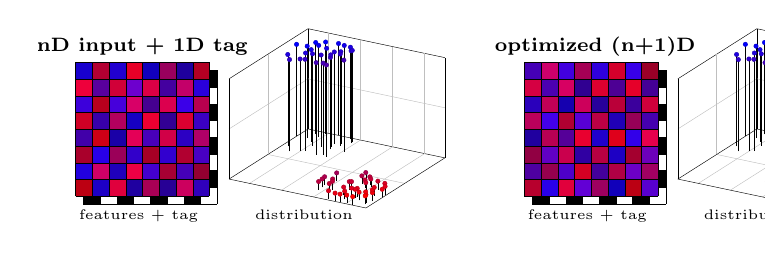
\begin{tikzpicture}
				% Target + tag
				\begin{scope}[shift={(6.5,0.0)}]
					\begin{scope}[shift={(0.0,0.0)}]
						\draw (0.85, 1.5) node[anchor=center] {\scriptsize \textbf{nD input + 1D tag}};

						\begin{scope}[shift={(0.1,-0.5)}, scale=1.7]
							\fill[fill={rgb,255:red,0; green,0; blue,0}]  (0.0,0.0) -- (0.125,0.0) -- (0.125,0.125) -- (0.0,0.125);
\fill[fill={rgb,255:red,255; green,255; blue,255}]  (0.0,0.125) -- (0.125,0.125) -- (0.125,0.25) -- (0.0,0.25);
\fill[fill={rgb,255:red,0; green,0; blue,0}]  (0.0,0.25) -- (0.125,0.25) -- (0.125,0.375) -- (0.0,0.375);
\fill[fill={rgb,255:red,255; green,255; blue,255}]  (0.0,0.375) -- (0.125,0.375) -- (0.125,0.5) -- (0.0,0.5);
\fill[fill={rgb,255:red,0; green,0; blue,0}]  (0.0,0.5) -- (0.125,0.5) -- (0.125,0.625) -- (0.0,0.625);
\fill[fill={rgb,255:red,255; green,255; blue,255}]  (0.0,0.625) -- (0.125,0.625) -- (0.125,0.75) -- (0.0,0.75);
\fill[fill={rgb,255:red,0; green,0; blue,0}]  (0.0,0.75) -- (0.125,0.75) -- (0.125,0.875) -- (0.0,0.875);
\fill[fill={rgb,255:red,255; green,255; blue,255}]  (0.0,0.875) -- (0.125,0.875) -- (0.125,1.0) -- (0.0,1.0);
\fill[fill={rgb,255:red,255; green,255; blue,255}]  (0.125,0.0) -- (0.25,0.0) -- (0.25,0.125) -- (0.125,0.125);
\fill[fill={rgb,255:red,0; green,0; blue,0}]  (0.125,0.125) -- (0.25,0.125) -- (0.25,0.25) -- (0.125,0.25);
\fill[fill={rgb,255:red,255; green,255; blue,255}]  (0.125,0.25) -- (0.25,0.25) -- (0.25,0.375) -- (0.125,0.375);
\fill[fill={rgb,255:red,0; green,0; blue,0}]  (0.125,0.375) -- (0.25,0.375) -- (0.25,0.5) -- (0.125,0.5);
\fill[fill={rgb,255:red,255; green,255; blue,255}]  (0.125,0.5) -- (0.25,0.5) -- (0.25,0.625) -- (0.125,0.625);
\fill[fill={rgb,255:red,0; green,0; blue,0}]  (0.125,0.625) -- (0.25,0.625) -- (0.25,0.75) -- (0.125,0.75);
\fill[fill={rgb,255:red,255; green,255; blue,255}]  (0.125,0.75) -- (0.25,0.75) -- (0.25,0.875) -- (0.125,0.875);
\fill[fill={rgb,255:red,0; green,0; blue,0}]  (0.125,0.875) -- (0.25,0.875) -- (0.25,1.0) -- (0.125,1.0);
\fill[fill={rgb,255:red,0; green,0; blue,0}]  (0.25,0.0) -- (0.375,0.0) -- (0.375,0.125) -- (0.25,0.125);
\fill[fill={rgb,255:red,255; green,255; blue,255}]  (0.25,0.125) -- (0.375,0.125) -- (0.375,0.25) -- (0.25,0.25);
\fill[fill={rgb,255:red,0; green,0; blue,0}]  (0.25,0.25) -- (0.375,0.25) -- (0.375,0.375) -- (0.25,0.375);
\fill[fill={rgb,255:red,255; green,255; blue,255}]  (0.25,0.375) -- (0.375,0.375) -- (0.375,0.5) -- (0.25,0.5);
\fill[fill={rgb,255:red,0; green,0; blue,0}]  (0.25,0.5) -- (0.375,0.5) -- (0.375,0.625) -- (0.25,0.625);
\fill[fill={rgb,255:red,255; green,255; blue,255}]  (0.25,0.625) -- (0.375,0.625) -- (0.375,0.75) -- (0.25,0.75);
\fill[fill={rgb,255:red,0; green,0; blue,0}]  (0.25,0.75) -- (0.375,0.75) -- (0.375,0.875) -- (0.25,0.875);
\fill[fill={rgb,255:red,255; green,255; blue,255}]  (0.25,0.875) -- (0.375,0.875) -- (0.375,1.0) -- (0.25,1.0);
\fill[fill={rgb,255:red,255; green,255; blue,255}]  (0.375,0.0) -- (0.5,0.0) -- (0.5,0.125) -- (0.375,0.125);
\fill[fill={rgb,255:red,0; green,0; blue,0}]  (0.375,0.125) -- (0.5,0.125) -- (0.5,0.25) -- (0.375,0.25);
\fill[fill={rgb,255:red,255; green,255; blue,255}]  (0.375,0.25) -- (0.5,0.25) -- (0.5,0.375) -- (0.375,0.375);
\fill[fill={rgb,255:red,0; green,0; blue,0}]  (0.375,0.375) -- (0.5,0.375) -- (0.5,0.5) -- (0.375,0.5);
\fill[fill={rgb,255:red,255; green,255; blue,255}]  (0.375,0.5) -- (0.5,0.5) -- (0.5,0.625) -- (0.375,0.625);
\fill[fill={rgb,255:red,0; green,0; blue,0}]  (0.375,0.625) -- (0.5,0.625) -- (0.5,0.75) -- (0.375,0.75);
\fill[fill={rgb,255:red,255; green,255; blue,255}]  (0.375,0.75) -- (0.5,0.75) -- (0.5,0.875) -- (0.375,0.875);
\fill[fill={rgb,255:red,0; green,0; blue,0}]  (0.375,0.875) -- (0.5,0.875) -- (0.5,1.0) -- (0.375,1.0);
\fill[fill={rgb,255:red,0; green,0; blue,0}]  (0.5,0.0) -- (0.625,0.0) -- (0.625,0.125) -- (0.5,0.125);
\fill[fill={rgb,255:red,255; green,255; blue,255}]  (0.5,0.125) -- (0.625,0.125) -- (0.625,0.25) -- (0.5,0.25);
\fill[fill={rgb,255:red,0; green,0; blue,0}]  (0.5,0.25) -- (0.625,0.25) -- (0.625,0.375) -- (0.5,0.375);
\fill[fill={rgb,255:red,255; green,255; blue,255}]  (0.5,0.375) -- (0.625,0.375) -- (0.625,0.5) -- (0.5,0.5);
\fill[fill={rgb,255:red,0; green,0; blue,0}]  (0.5,0.5) -- (0.625,0.5) -- (0.625,0.625) -- (0.5,0.625);
\fill[fill={rgb,255:red,255; green,255; blue,255}]  (0.5,0.625) -- (0.625,0.625) -- (0.625,0.75) -- (0.5,0.75);
\fill[fill={rgb,255:red,0; green,0; blue,0}]  (0.5,0.75) -- (0.625,0.75) -- (0.625,0.875) -- (0.5,0.875);
\fill[fill={rgb,255:red,255; green,255; blue,255}]  (0.5,0.875) -- (0.625,0.875) -- (0.625,1.0) -- (0.5,1.0);
\fill[fill={rgb,255:red,255; green,255; blue,255}]  (0.625,0.0) -- (0.75,0.0) -- (0.75,0.125) -- (0.625,0.125);
\fill[fill={rgb,255:red,0; green,0; blue,0}]  (0.625,0.125) -- (0.75,0.125) -- (0.75,0.25) -- (0.625,0.25);
\fill[fill={rgb,255:red,255; green,255; blue,255}]  (0.625,0.25) -- (0.75,0.25) -- (0.75,0.375) -- (0.625,0.375);
\fill[fill={rgb,255:red,0; green,0; blue,0}]  (0.625,0.375) -- (0.75,0.375) -- (0.75,0.5) -- (0.625,0.5);
\fill[fill={rgb,255:red,255; green,255; blue,255}]  (0.625,0.5) -- (0.75,0.5) -- (0.75,0.625) -- (0.625,0.625);
\fill[fill={rgb,255:red,0; green,0; blue,0}]  (0.625,0.625) -- (0.75,0.625) -- (0.75,0.75) -- (0.625,0.75);
\fill[fill={rgb,255:red,255; green,255; blue,255}]  (0.625,0.75) -- (0.75,0.75) -- (0.75,0.875) -- (0.625,0.875);
\fill[fill={rgb,255:red,0; green,0; blue,0}]  (0.625,0.875) -- (0.75,0.875) -- (0.75,1.0) -- (0.625,1.0);
\fill[fill={rgb,255:red,0; green,0; blue,0}]  (0.75,0.0) -- (0.875,0.0) -- (0.875,0.125) -- (0.75,0.125);
\fill[fill={rgb,255:red,255; green,255; blue,255}]  (0.75,0.125) -- (0.875,0.125) -- (0.875,0.25) -- (0.75,0.25);
\fill[fill={rgb,255:red,0; green,0; blue,0}]  (0.75,0.25) -- (0.875,0.25) -- (0.875,0.375) -- (0.75,0.375);
\fill[fill={rgb,255:red,255; green,255; blue,255}]  (0.75,0.375) -- (0.875,0.375) -- (0.875,0.5) -- (0.75,0.5);
\fill[fill={rgb,255:red,0; green,0; blue,0}]  (0.75,0.5) -- (0.875,0.5) -- (0.875,0.625) -- (0.75,0.625);
\fill[fill={rgb,255:red,255; green,255; blue,255}]  (0.75,0.625) -- (0.875,0.625) -- (0.875,0.75) -- (0.75,0.75);
\fill[fill={rgb,255:red,0; green,0; blue,0}]  (0.75,0.75) -- (0.875,0.75) -- (0.875,0.875) -- (0.75,0.875);
\fill[fill={rgb,255:red,255; green,255; blue,255}]  (0.75,0.875) -- (0.875,0.875) -- (0.875,1.0) -- (0.75,1.0);
\fill[fill={rgb,255:red,255; green,255; blue,255}]  (0.875,0.0) -- (1.0,0.0) -- (1.0,0.125) -- (0.875,0.125);
\fill[fill={rgb,255:red,0; green,0; blue,0}]  (0.875,0.125) -- (1.0,0.125) -- (1.0,0.25) -- (0.875,0.25);
\fill[fill={rgb,255:red,255; green,255; blue,255}]  (0.875,0.25) -- (1.0,0.25) -- (1.0,0.375) -- (0.875,0.375);
\fill[fill={rgb,255:red,0; green,0; blue,0}]  (0.875,0.375) -- (1.0,0.375) -- (1.0,0.5) -- (0.875,0.5);
\fill[fill={rgb,255:red,255; green,255; blue,255}]  (0.875,0.5) -- (1.0,0.5) -- (1.0,0.625) -- (0.875,0.625);
\fill[fill={rgb,255:red,0; green,0; blue,0}]  (0.875,0.625) -- (1.0,0.625) -- (1.0,0.75) -- (0.875,0.75);
\fill[fill={rgb,255:red,255; green,255; blue,255}]  (0.875,0.75) -- (1.0,0.75) -- (1.0,0.875) -- (0.875,0.875);
\fill[fill={rgb,255:red,0; green,0; blue,0}]  (0.875,0.875) -- (1.0,0.875) -- (1.0,1.0) -- (0.875,1.0);

\draw[black, -, line width = 0.1] (0,0.0) -- (1,0.0);
\draw[black, -, line width = 0.1] (0.0, 0) -- (0.0, 1);
\draw[black, -, line width = 0.1] (0,0.125) -- (1,0.125);
\draw[black, -, line width = 0.1] (0.125, 0) -- (0.125, 1);
\draw[black, -, line width = 0.1] (0,0.25) -- (1,0.25);
\draw[black, -, line width = 0.1] (0.25, 0) -- (0.25, 1);
\draw[black, -, line width = 0.1] (0,0.375) -- (1,0.375);
\draw[black, -, line width = 0.1] (0.375, 0) -- (0.375, 1);
\draw[black, -, line width = 0.1] (0,0.5) -- (1,0.5);
\draw[black, -, line width = 0.1] (0.5, 0) -- (0.5, 1);
\draw[black, -, line width = 0.1] (0,0.625) -- (1,0.625);
\draw[black, -, line width = 0.1] (0.625, 0) -- (0.625, 1);
\draw[black, -, line width = 0.1] (0,0.75) -- (1,0.75);
\draw[black, -, line width = 0.1] (0.75, 0) -- (0.75, 1);
\draw[black, -, line width = 0.1] (0,0.875) -- (1,0.875);
\draw[black, -, line width = 0.1] (0.875, 0) -- (0.875, 1);
\draw[black, -, line width = 0.1] (0,1.0) -- (1,1.0);
\draw[black, -, line width = 0.1] (1.0, 0) -- (1.0, 1);
						\end{scope}
						\begin{scope}[shift={(0.0,-0.4)}, scale=1.7]
							\fill[fill={rgb,255:red,188; green,0; blue,18}]  (0.0,0.0) -- (0.125,0.0) -- (0.125,0.125) -- (0.0,0.125);
\fill[fill={rgb,255:red,34; green,0; blue,222}]  (0.0,0.125) -- (0.125,0.125) -- (0.125,0.25) -- (0.0,0.25);
\fill[fill={rgb,255:red,169; green,0; blue,43}]  (0.0,0.25) -- (0.125,0.25) -- (0.125,0.375) -- (0.0,0.375);
\fill[fill={rgb,255:red,65; green,0; blue,169}]  (0.0,0.375) -- (0.125,0.375) -- (0.125,0.5) -- (0.0,0.5);
\fill[fill={rgb,255:red,208; green,0; blue,37}]  (0.0,0.5) -- (0.125,0.5) -- (0.125,0.625) -- (0.0,0.625);
\fill[fill={rgb,255:red,60; green,0; blue,219}]  (0.0,0.625) -- (0.125,0.625) -- (0.125,0.75) -- (0.0,0.75);
\fill[fill={rgb,255:red,238; green,0; blue,59}]  (0.0,0.75) -- (0.125,0.75) -- (0.125,0.875) -- (0.0,0.875);
\fill[fill={rgb,255:red,24; green,0; blue,206}]  (0.0,0.875) -- (0.125,0.875) -- (0.125,1.0) -- (0.0,1.0);
\fill[fill={rgb,255:red,29; green,0; blue,197}]  (0.125,0.0) -- (0.25,0.0) -- (0.25,0.125) -- (0.125,0.125);
\fill[fill={rgb,255:red,207; green,0; blue,102}]  (0.125,0.125) -- (0.25,0.125) -- (0.25,0.25) -- (0.125,0.25);
\fill[fill={rgb,255:red,40; green,0; blue,232}]  (0.125,0.25) -- (0.25,0.25) -- (0.25,0.375) -- (0.125,0.375);
\fill[fill={rgb,255:red,206; green,0; blue,22}]  (0.125,0.375) -- (0.25,0.375) -- (0.25,0.5) -- (0.125,0.5);
\fill[fill={rgb,255:red,56; green,0; blue,170}]  (0.125,0.5) -- (0.25,0.5) -- (0.25,0.625) -- (0.125,0.625);
\fill[fill={rgb,255:red,184; green,0; blue,29}]  (0.125,0.625) -- (0.25,0.625) -- (0.25,0.75) -- (0.125,0.75);
\fill[fill={rgb,255:red,89; green,0; blue,158}]  (0.125,0.75) -- (0.25,0.75) -- (0.25,0.875) -- (0.125,0.875);
\fill[fill={rgb,255:red,178; green,0; blue,50}]  (0.125,0.875) -- (0.25,0.875) -- (0.25,1.0) -- (0.125,1.0);
\fill[fill={rgb,255:red,224; green,0; blue,61}]  (0.25,0.0) -- (0.375,0.0) -- (0.375,0.125) -- (0.25,0.125);
\fill[fill={rgb,255:red,31; green,0; blue,187}]  (0.25,0.125) -- (0.375,0.125) -- (0.375,0.25) -- (0.25,0.25);
\fill[fill={rgb,255:red,155; green,0; blue,89}]  (0.25,0.25) -- (0.375,0.25) -- (0.375,0.375) -- (0.25,0.375);
\fill[fill={rgb,255:red,26; green,0; blue,167}]  (0.25,0.375) -- (0.375,0.375) -- (0.375,0.5) -- (0.25,0.5);
\fill[fill={rgb,255:red,178; green,0; blue,94}]  (0.25,0.5) -- (0.375,0.5) -- (0.375,0.625) -- (0.25,0.625);
\fill[fill={rgb,255:red,70; green,0; blue,219}]  (0.25,0.625) -- (0.375,0.625) -- (0.375,0.75) -- (0.25,0.75);
\fill[fill={rgb,255:red,209; green,0; blue,56}]  (0.25,0.75) -- (0.375,0.75) -- (0.375,0.875) -- (0.25,0.875);
\fill[fill={rgb,255:red,33; green,0; blue,208}]  (0.25,0.875) -- (0.375,0.875) -- (0.375,1.0) -- (0.25,1.0);
\fill[fill={rgb,255:red,31; green,0; blue,160}]  (0.375,0.0) -- (0.5,0.0) -- (0.5,0.125) -- (0.375,0.125);
\fill[fill={rgb,255:red,237; green,0; blue,68}]  (0.375,0.125) -- (0.5,0.125) -- (0.5,0.25) -- (0.375,0.25);
\fill[fill={rgb,255:red,50; green,0; blue,202}]  (0.375,0.25) -- (0.5,0.25) -- (0.5,0.375) -- (0.375,0.375);
\fill[fill={rgb,255:red,228; green,0; blue,87}]  (0.375,0.375) -- (0.5,0.375) -- (0.5,0.5) -- (0.375,0.5);
\fill[fill={rgb,255:red,22; green,0; blue,195}]  (0.375,0.5) -- (0.5,0.5) -- (0.5,0.625) -- (0.375,0.625);
\fill[fill={rgb,255:red,216; green,0; blue,103}]  (0.375,0.625) -- (0.5,0.625) -- (0.5,0.75) -- (0.375,0.75);
\fill[fill={rgb,255:red,109; green,0; blue,206}]  (0.375,0.75) -- (0.5,0.75) -- (0.5,0.875) -- (0.375,0.875);
\fill[fill={rgb,255:red,231; green,0; blue,39}]  (0.375,0.875) -- (0.5,0.875) -- (0.5,1.0) -- (0.375,1.0);
\fill[fill={rgb,255:red,168; green,0; blue,85}]  (0.5,0.0) -- (0.625,0.0) -- (0.625,0.125) -- (0.5,0.125);
\fill[fill={rgb,255:red,68; green,0; blue,207}]  (0.5,0.125) -- (0.625,0.125) -- (0.625,0.25) -- (0.5,0.25);
\fill[fill={rgb,255:red,166; green,0; blue,37}]  (0.5,0.25) -- (0.625,0.25) -- (0.625,0.375) -- (0.5,0.375);
\fill[fill={rgb,255:red,72; green,0; blue,186}]  (0.5,0.375) -- (0.625,0.375) -- (0.625,0.5) -- (0.5,0.5);
\fill[fill={rgb,255:red,236; green,0; blue,49}]  (0.5,0.5) -- (0.625,0.5) -- (0.625,0.625) -- (0.5,0.625);
\fill[fill={rgb,255:red,69; green,0; blue,145}]  (0.5,0.625) -- (0.625,0.625) -- (0.625,0.75) -- (0.5,0.75);
\fill[fill={rgb,255:red,220; green,0; blue,69}]  (0.5,0.75) -- (0.625,0.75) -- (0.625,0.875) -- (0.5,0.875);
\fill[fill={rgb,255:red,18; green,0; blue,188}]  (0.5,0.875) -- (0.625,0.875) -- (0.625,1.0) -- (0.5,1.0);
\fill[fill={rgb,255:red,39; green,0; blue,149}]  (0.625,0.0) -- (0.75,0.0) -- (0.75,0.125) -- (0.625,0.125);
\fill[fill={rgb,255:red,166; green,0; blue,51}]  (0.625,0.125) -- (0.75,0.125) -- (0.75,0.25) -- (0.625,0.25);
\fill[fill={rgb,255:red,50; green,0; blue,207}]  (0.625,0.25) -- (0.75,0.25) -- (0.75,0.375) -- (0.625,0.375);
\fill[fill={rgb,255:red,209; green,0; blue,71}]  (0.625,0.375) -- (0.75,0.375) -- (0.75,0.5) -- (0.625,0.5);
\fill[fill={rgb,255:red,50; green,0; blue,148}]  (0.625,0.5) -- (0.75,0.5) -- (0.75,0.625) -- (0.625,0.625);
\fill[fill={rgb,255:red,220; green,0; blue,78}]  (0.625,0.625) -- (0.75,0.625) -- (0.75,0.75) -- (0.625,0.75);
\fill[fill={rgb,255:red,68; green,0; blue,159}]  (0.625,0.75) -- (0.75,0.75) -- (0.75,0.875) -- (0.625,0.875);
\fill[fill={rgb,255:red,153; green,0; blue,93}]  (0.625,0.875) -- (0.75,0.875) -- (0.75,1.0) -- (0.625,1.0);
\fill[fill={rgb,255:red,204; green,0; blue,94}]  (0.75,0.0) -- (0.875,0.0) -- (0.875,0.125) -- (0.75,0.125);
\fill[fill={rgb,255:red,69; green,0; blue,184}]  (0.75,0.125) -- (0.875,0.125) -- (0.875,0.25) -- (0.75,0.25);
\fill[fill={rgb,255:red,177; green,0; blue,48}]  (0.75,0.25) -- (0.875,0.25) -- (0.875,0.375) -- (0.75,0.375);
\fill[fill={rgb,255:red,44; green,0; blue,195}]  (0.75,0.375) -- (0.875,0.375) -- (0.875,0.5) -- (0.75,0.5);
\fill[fill={rgb,255:red,220; green,0; blue,48}]  (0.75,0.5) -- (0.875,0.5) -- (0.875,0.625) -- (0.75,0.625);
\fill[fill={rgb,255:red,59; green,0; blue,232}]  (0.75,0.625) -- (0.875,0.625) -- (0.875,0.75) -- (0.75,0.75);
\fill[fill={rgb,255:red,195; green,0; blue,105}]  (0.75,0.75) -- (0.875,0.75) -- (0.875,0.875) -- (0.75,0.875);
\fill[fill={rgb,255:red,31; green,0; blue,158}]  (0.75,0.875) -- (0.875,0.875) -- (0.875,1.0) -- (0.75,1.0);
\fill[fill={rgb,255:red,48; green,0; blue,187}]  (0.875,0.0) -- (1.0,0.0) -- (1.0,0.125) -- (0.875,0.125);
\fill[fill={rgb,255:red,148; green,0; blue,49}]  (0.875,0.125) -- (1.0,0.125) -- (1.0,0.25) -- (0.875,0.25);
\fill[fill={rgb,255:red,72; green,0; blue,196}]  (0.875,0.25) -- (1.0,0.25) -- (1.0,0.375) -- (0.875,0.375);
\fill[fill={rgb,255:red,177; green,0; blue,103}]  (0.875,0.375) -- (1.0,0.375) -- (1.0,0.5) -- (0.875,0.5);
\fill[fill={rgb,255:red,59; green,0; blue,194}]  (0.875,0.5) -- (1.0,0.5) -- (1.0,0.625) -- (0.875,0.625);
\fill[fill={rgb,255:red,184; green,0; blue,78}]  (0.875,0.625) -- (1.0,0.625) -- (1.0,0.75) -- (0.875,0.75);
\fill[fill={rgb,255:red,42; green,0; blue,219}]  (0.875,0.75) -- (1.0,0.75) -- (1.0,0.875) -- (0.875,0.875);
\fill[fill={rgb,255:red,179; green,0; blue,35}]  (0.875,0.875) -- (1.0,0.875) -- (1.0,1.0) -- (0.875,1.0);
\draw[black, -, line width = 0.1] (0,0.0) -- (1,0.0);
\draw[black, -, line width = 0.1] (0.0, 0) -- (0.0, 1);
\draw[black, -, line width = 0.1] (0,0.125) -- (1,0.125);
\draw[black, -, line width = 0.1] (0.125, 0) -- (0.125, 1);
\draw[black, -, line width = 0.1] (0,0.25) -- (1,0.25);
\draw[black, -, line width = 0.1] (0.25, 0) -- (0.25, 1);
\draw[black, -, line width = 0.1] (0,0.375) -- (1,0.375);
\draw[black, -, line width = 0.1] (0.375, 0) -- (0.375, 1);
\draw[black, -, line width = 0.1] (0,0.5) -- (1,0.5);
\draw[black, -, line width = 0.1] (0.5, 0) -- (0.5, 1);
\draw[black, -, line width = 0.1] (0,0.625) -- (1,0.625);
\draw[black, -, line width = 0.1] (0.625, 0) -- (0.625, 1);
\draw[black, -, line width = 0.1] (0,0.75) -- (1,0.75);
\draw[black, -, line width = 0.1] (0.75, 0) -- (0.75, 1);
\draw[black, -, line width = 0.1] (0,0.875) -- (1,0.875);
\draw[black, -, line width = 0.1] (0.875, 0) -- (0.875, 1);
\draw[black, -, line width = 0.1] (0,1.0) -- (1,1.0);
\draw[black, -, line width = 0.1] (1.0, 0) -- (1.0, 1);
						\end{scope}

						% Plots
						\begin{scope}[shift={(1.95,-0.55)}, scale=0.4]
							\begin{axis}[grid=major,
             view={210}{30},
             ticks=none,
            ]
	\addplot3[only marks, ycomb, scatter,colormap name=mine,point meta=x-y,domain=0:1] 
		coordinates {
( 0.7375242851479528 , 0.07149719324412154 , 0.8 )
( 0.6352616126167896 , 0.3741453717776989 , 0.8 )
( 0.6659961465969623 , 0.16905674183969271 , 0.8 )
( 0.7581160815510639 , 0.1634410081431301 , 0.8 )
( 0.8163931968005627 , 0.14827914918912766 , 0.8 )
( 0.235522015159636 , 0.862679580008819 , 0.2 )
( 0.4358410694203565 , 0.7349179605485335 , 0.2 )
( 0.09431609762856191 , 0.808318117172903 , 0.2 )
( 0.1154706312820831 , 0.7728239727237151 , 0.2 )
( 0.3139804373163412 , 0.9008613797149576 , 0.2 )
( 0.157427062376505 , 0.9106254691891366 , 0.2 )
( 0.8087453710717747 , 0.0873358066465128 , 0.8 )
( 0.22286168569889056 , 0.6672178044029601 , 0.2 )
( 0.22297990357259065 , 0.6156022713570786 , 0.2 )
( 0.8516233378780766 , 0.11998168903668985 , 0.8 )
( 0.19926435538276854 , 0.6994255744573358 , 0.2 )
( 0.38176637786578715 , 0.7412614969652668 , 0.2 )
( 0.12451618465828287 , 0.7369979876185243 , 0.2 )
( 0.10979748007965975 , 0.8512815509980239 , 0.2 )
( 0.10479225209789506 , 0.6579663171400711 , 0.2 )
( 0.7009834334711795 , 0.3720120811638443 , 0.8 )
( 0.7773961056233383 , 0.3599495053784583 , 0.8 )
( 0.8201340945592945 , 0.22151647062355037 , 0.8 )
( 0.131654833648978 , 0.816398412146849 , 0.2 )
( 0.6245513907080336 , 0.13009483281432893 , 0.8 )
( 0.430694727643888 , 0.7696278088773739 , 0.2 )
( 0.1972961888949818 , 0.7946443747181786 , 0.2 )
( 0.8941919835488764 , 0.3450755917066442 , 0.8 )
( 0.5897943690388352 , 0.26685768854268516 , 0.8 )
( 0.8482706859776603 , 0.404644785626021 , 0.8 )
( 0.4284911662411657 , 0.8111718300538617 , 0.2 )
( 0.4076415266589243 , 0.6543043974677796 , 0.2 )
( 0.16102372309131766 , 0.8368607468802273 , 0.2 )
( 0.2701167616942569 , 0.8142574315792738 , 0.2 )
( 0.1539149012676253 , 0.6483720921974706 , 0.2 )
( 0.2841292635125761 , 0.7305270744563124 , 0.2 )
( 0.9277902148119016 , 0.1938935051088681 , 0.8 )
( 0.27391219388005256 , 0.5725148987449746 , 0.2 )
( 0.36551326907490445 , 0.7713106951700408 , 0.2 )
( 0.0734335217243964 , 0.7396019784732524 , 0.2 )
( 0.6543978342157951 , 0.08650271025822998 , 0.8 )
( 0.6512898381036001 , 0.2000216613180242 , 0.8 )
( 0.1995156704890989 , 0.8120878635117923 , 0.2 )
( 0.821622311898793 , 0.2790205918520516 , 0.8 )
( 0.6962408637146551 , 0.08076108729329323 , 0.8 )
( 0.3636534200400908 , 0.8083595677085642 , 0.2 )
( 0.2679208190322526 , 0.6244303950353428 , 0.2 )
( 0.10389673801250013 , 0.8681040527778956 , 0.2 )
( 0.8033544609775752 , 0.36867725590955347 , 0.8 )
( 0.2740573751979177 , 0.7243578756697717 , 0.2 )
( 0.6948557533715101 , 0.18925959140395698 , 0.8 )
( 0.6728557525654665 , 0.2679928808749045 , 0.8 )
( 0.8647811959996955 , 0.18825570536856379 , 0.8 )
( 0.23518869693404476 , 0.9128898340829545 , 0.2 )
( 0.265926429611197 , 0.9133710202209234 , 0.2 )
( 0.6220106906020064 , 0.1219079342588435 , 0.8 )
( 0.6902126391538932 , 0.23480703283724697 , 0.8 )
( 0.08131589045249188 , 0.6954331462900474 , 0.2 )
( 0.7832485755015384 , 0.2709581697935482 , 0.8 )
( 0.19700724066228567 , 0.9067820388330438 , 0.2 )
( 0.7340980139455315 , 0.2627891475368584 , 0.8 )
( 0.22544026580990742 , 0.806029256851962 , 0.2 )
( 0.6648862020343914 , 0.3593651794811017 , 0.8 )
( 0.20270234187784264 , 0.640557176544345 , 0.2 )
       };
	\end{axis}
						\end{scope}
						\draw[anchor=north] (0.8,-0.45) node {\tiny features + tag};
						\draw[anchor=north] (2.9,-0.45) node {\tiny distribution};
					\end{scope}
					\hspace{20mm}
					% Target + tag
					\begin{scope}[shift={(3.70,0.0)}]
						\draw (0.9, 1.5) node[anchor=center] {\scriptsize \textbf{optimized (n+1)D}};

						\begin{scope}[shift={(0.1,-0.5)}, scale=1.7]
							\fill[fill={rgb,255:red,0; green,0; blue,0}]  (0.0,0.0) -- (0.125,0.0) -- (0.125,0.125) -- (0.0,0.125);
\fill[fill={rgb,255:red,255; green,255; blue,255}]  (0.0,0.125) -- (0.125,0.125) -- (0.125,0.25) -- (0.0,0.25);
\fill[fill={rgb,255:red,0; green,0; blue,0}]  (0.0,0.25) -- (0.125,0.25) -- (0.125,0.375) -- (0.0,0.375);
\fill[fill={rgb,255:red,255; green,255; blue,255}]  (0.0,0.375) -- (0.125,0.375) -- (0.125,0.5) -- (0.0,0.5);
\fill[fill={rgb,255:red,0; green,0; blue,0}]  (0.0,0.5) -- (0.125,0.5) -- (0.125,0.625) -- (0.0,0.625);
\fill[fill={rgb,255:red,255; green,255; blue,255}]  (0.0,0.625) -- (0.125,0.625) -- (0.125,0.75) -- (0.0,0.75);
\fill[fill={rgb,255:red,0; green,0; blue,0}]  (0.0,0.75) -- (0.125,0.75) -- (0.125,0.875) -- (0.0,0.875);
\fill[fill={rgb,255:red,255; green,255; blue,255}]  (0.0,0.875) -- (0.125,0.875) -- (0.125,1.0) -- (0.0,1.0);
\fill[fill={rgb,255:red,255; green,255; blue,255}]  (0.125,0.0) -- (0.25,0.0) -- (0.25,0.125) -- (0.125,0.125);
\fill[fill={rgb,255:red,0; green,0; blue,0}]  (0.125,0.125) -- (0.25,0.125) -- (0.25,0.25) -- (0.125,0.25);
\fill[fill={rgb,255:red,255; green,255; blue,255}]  (0.125,0.25) -- (0.25,0.25) -- (0.25,0.375) -- (0.125,0.375);
\fill[fill={rgb,255:red,0; green,0; blue,0}]  (0.125,0.375) -- (0.25,0.375) -- (0.25,0.5) -- (0.125,0.5);
\fill[fill={rgb,255:red,255; green,255; blue,255}]  (0.125,0.5) -- (0.25,0.5) -- (0.25,0.625) -- (0.125,0.625);
\fill[fill={rgb,255:red,0; green,0; blue,0}]  (0.125,0.625) -- (0.25,0.625) -- (0.25,0.75) -- (0.125,0.75);
\fill[fill={rgb,255:red,255; green,255; blue,255}]  (0.125,0.75) -- (0.25,0.75) -- (0.25,0.875) -- (0.125,0.875);
\fill[fill={rgb,255:red,0; green,0; blue,0}]  (0.125,0.875) -- (0.25,0.875) -- (0.25,1.0) -- (0.125,1.0);
\fill[fill={rgb,255:red,0; green,0; blue,0}]  (0.25,0.0) -- (0.375,0.0) -- (0.375,0.125) -- (0.25,0.125);
\fill[fill={rgb,255:red,255; green,255; blue,255}]  (0.25,0.125) -- (0.375,0.125) -- (0.375,0.25) -- (0.25,0.25);
\fill[fill={rgb,255:red,0; green,0; blue,0}]  (0.25,0.25) -- (0.375,0.25) -- (0.375,0.375) -- (0.25,0.375);
\fill[fill={rgb,255:red,255; green,255; blue,255}]  (0.25,0.375) -- (0.375,0.375) -- (0.375,0.5) -- (0.25,0.5);
\fill[fill={rgb,255:red,0; green,0; blue,0}]  (0.25,0.5) -- (0.375,0.5) -- (0.375,0.625) -- (0.25,0.625);
\fill[fill={rgb,255:red,255; green,255; blue,255}]  (0.25,0.625) -- (0.375,0.625) -- (0.375,0.75) -- (0.25,0.75);
\fill[fill={rgb,255:red,0; green,0; blue,0}]  (0.25,0.75) -- (0.375,0.75) -- (0.375,0.875) -- (0.25,0.875);
\fill[fill={rgb,255:red,255; green,255; blue,255}]  (0.25,0.875) -- (0.375,0.875) -- (0.375,1.0) -- (0.25,1.0);
\fill[fill={rgb,255:red,255; green,255; blue,255}]  (0.375,0.0) -- (0.5,0.0) -- (0.5,0.125) -- (0.375,0.125);
\fill[fill={rgb,255:red,0; green,0; blue,0}]  (0.375,0.125) -- (0.5,0.125) -- (0.5,0.25) -- (0.375,0.25);
\fill[fill={rgb,255:red,255; green,255; blue,255}]  (0.375,0.25) -- (0.5,0.25) -- (0.5,0.375) -- (0.375,0.375);
\fill[fill={rgb,255:red,0; green,0; blue,0}]  (0.375,0.375) -- (0.5,0.375) -- (0.5,0.5) -- (0.375,0.5);
\fill[fill={rgb,255:red,255; green,255; blue,255}]  (0.375,0.5) -- (0.5,0.5) -- (0.5,0.625) -- (0.375,0.625);
\fill[fill={rgb,255:red,0; green,0; blue,0}]  (0.375,0.625) -- (0.5,0.625) -- (0.5,0.75) -- (0.375,0.75);
\fill[fill={rgb,255:red,255; green,255; blue,255}]  (0.375,0.75) -- (0.5,0.75) -- (0.5,0.875) -- (0.375,0.875);
\fill[fill={rgb,255:red,0; green,0; blue,0}]  (0.375,0.875) -- (0.5,0.875) -- (0.5,1.0) -- (0.375,1.0);
\fill[fill={rgb,255:red,0; green,0; blue,0}]  (0.5,0.0) -- (0.625,0.0) -- (0.625,0.125) -- (0.5,0.125);
\fill[fill={rgb,255:red,255; green,255; blue,255}]  (0.5,0.125) -- (0.625,0.125) -- (0.625,0.25) -- (0.5,0.25);
\fill[fill={rgb,255:red,0; green,0; blue,0}]  (0.5,0.25) -- (0.625,0.25) -- (0.625,0.375) -- (0.5,0.375);
\fill[fill={rgb,255:red,255; green,255; blue,255}]  (0.5,0.375) -- (0.625,0.375) -- (0.625,0.5) -- (0.5,0.5);
\fill[fill={rgb,255:red,0; green,0; blue,0}]  (0.5,0.5) -- (0.625,0.5) -- (0.625,0.625) -- (0.5,0.625);
\fill[fill={rgb,255:red,255; green,255; blue,255}]  (0.5,0.625) -- (0.625,0.625) -- (0.625,0.75) -- (0.5,0.75);
\fill[fill={rgb,255:red,0; green,0; blue,0}]  (0.5,0.75) -- (0.625,0.75) -- (0.625,0.875) -- (0.5,0.875);
\fill[fill={rgb,255:red,255; green,255; blue,255}]  (0.5,0.875) -- (0.625,0.875) -- (0.625,1.0) -- (0.5,1.0);
\fill[fill={rgb,255:red,255; green,255; blue,255}]  (0.625,0.0) -- (0.75,0.0) -- (0.75,0.125) -- (0.625,0.125);
\fill[fill={rgb,255:red,0; green,0; blue,0}]  (0.625,0.125) -- (0.75,0.125) -- (0.75,0.25) -- (0.625,0.25);
\fill[fill={rgb,255:red,255; green,255; blue,255}]  (0.625,0.25) -- (0.75,0.25) -- (0.75,0.375) -- (0.625,0.375);
\fill[fill={rgb,255:red,0; green,0; blue,0}]  (0.625,0.375) -- (0.75,0.375) -- (0.75,0.5) -- (0.625,0.5);
\fill[fill={rgb,255:red,255; green,255; blue,255}]  (0.625,0.5) -- (0.75,0.5) -- (0.75,0.625) -- (0.625,0.625);
\fill[fill={rgb,255:red,0; green,0; blue,0}]  (0.625,0.625) -- (0.75,0.625) -- (0.75,0.75) -- (0.625,0.75);
\fill[fill={rgb,255:red,255; green,255; blue,255}]  (0.625,0.75) -- (0.75,0.75) -- (0.75,0.875) -- (0.625,0.875);
\fill[fill={rgb,255:red,0; green,0; blue,0}]  (0.625,0.875) -- (0.75,0.875) -- (0.75,1.0) -- (0.625,1.0);
\fill[fill={rgb,255:red,0; green,0; blue,0}]  (0.75,0.0) -- (0.875,0.0) -- (0.875,0.125) -- (0.75,0.125);
\fill[fill={rgb,255:red,255; green,255; blue,255}]  (0.75,0.125) -- (0.875,0.125) -- (0.875,0.25) -- (0.75,0.25);
\fill[fill={rgb,255:red,0; green,0; blue,0}]  (0.75,0.25) -- (0.875,0.25) -- (0.875,0.375) -- (0.75,0.375);
\fill[fill={rgb,255:red,255; green,255; blue,255}]  (0.75,0.375) -- (0.875,0.375) -- (0.875,0.5) -- (0.75,0.5);
\fill[fill={rgb,255:red,0; green,0; blue,0}]  (0.75,0.5) -- (0.875,0.5) -- (0.875,0.625) -- (0.75,0.625);
\fill[fill={rgb,255:red,255; green,255; blue,255}]  (0.75,0.625) -- (0.875,0.625) -- (0.875,0.75) -- (0.75,0.75);
\fill[fill={rgb,255:red,0; green,0; blue,0}]  (0.75,0.75) -- (0.875,0.75) -- (0.875,0.875) -- (0.75,0.875);
\fill[fill={rgb,255:red,255; green,255; blue,255}]  (0.75,0.875) -- (0.875,0.875) -- (0.875,1.0) -- (0.75,1.0);
\fill[fill={rgb,255:red,255; green,255; blue,255}]  (0.875,0.0) -- (1.0,0.0) -- (1.0,0.125) -- (0.875,0.125);
\fill[fill={rgb,255:red,0; green,0; blue,0}]  (0.875,0.125) -- (1.0,0.125) -- (1.0,0.25) -- (0.875,0.25);
\fill[fill={rgb,255:red,255; green,255; blue,255}]  (0.875,0.25) -- (1.0,0.25) -- (1.0,0.375) -- (0.875,0.375);
\fill[fill={rgb,255:red,0; green,0; blue,0}]  (0.875,0.375) -- (1.0,0.375) -- (1.0,0.5) -- (0.875,0.5);
\fill[fill={rgb,255:red,255; green,255; blue,255}]  (0.875,0.5) -- (1.0,0.5) -- (1.0,0.625) -- (0.875,0.625);
\fill[fill={rgb,255:red,0; green,0; blue,0}]  (0.875,0.625) -- (1.0,0.625) -- (1.0,0.75) -- (0.875,0.75);
\fill[fill={rgb,255:red,255; green,255; blue,255}]  (0.875,0.75) -- (1.0,0.75) -- (1.0,0.875) -- (0.875,0.875);
\fill[fill={rgb,255:red,0; green,0; blue,0}]  (0.875,0.875) -- (1.0,0.875) -- (1.0,1.0) -- (0.875,1.0);

\draw[black, -, line width = 0.1] (0,0.0) -- (1,0.0);
\draw[black, -, line width = 0.1] (0.0, 0) -- (0.0, 1);
\draw[black, -, line width = 0.1] (0,0.125) -- (1,0.125);
\draw[black, -, line width = 0.1] (0.125, 0) -- (0.125, 1);
\draw[black, -, line width = 0.1] (0,0.25) -- (1,0.25);
\draw[black, -, line width = 0.1] (0.25, 0) -- (0.25, 1);
\draw[black, -, line width = 0.1] (0,0.375) -- (1,0.375);
\draw[black, -, line width = 0.1] (0.375, 0) -- (0.375, 1);
\draw[black, -, line width = 0.1] (0,0.5) -- (1,0.5);
\draw[black, -, line width = 0.1] (0.5, 0) -- (0.5, 1);
\draw[black, -, line width = 0.1] (0,0.625) -- (1,0.625);
\draw[black, -, line width = 0.1] (0.625, 0) -- (0.625, 1);
\draw[black, -, line width = 0.1] (0,0.75) -- (1,0.75);
\draw[black, -, line width = 0.1] (0.75, 0) -- (0.75, 1);
\draw[black, -, line width = 0.1] (0,0.875) -- (1,0.875);
\draw[black, -, line width = 0.1] (0.875, 0) -- (0.875, 1);
\draw[black, -, line width = 0.1] (0,1.0) -- (1,1.0);
\draw[black, -, line width = 0.1] (1.0, 0) -- (1.0, 1);
						\end{scope}
						\begin{scope}[shift={(0.0,-0.4)}, scale=1.7]
							\fill[fill={rgb,255:red,183; green,0; blue,45}]  (0.0,0.0) -- (0.125,0.0) -- (0.125,0.125) -- (0.0,0.125);
\fill[fill={rgb,255:red,78; green,0; blue,161}]  (0.0,0.125) -- (0.125,0.125) -- (0.125,0.25) -- (0.0,0.25);
\fill[fill={rgb,255:red,145; green,0; blue,67}]  (0.0,0.25) -- (0.125,0.25) -- (0.125,0.375) -- (0.0,0.375);
\fill[fill={rgb,255:red,32; green,0; blue,159}]  (0.0,0.375) -- (0.125,0.375) -- (0.125,0.5) -- (0.0,0.5);
\fill[fill={rgb,255:red,186; green,0; blue,91}]  (0.0,0.5) -- (0.125,0.5) -- (0.125,0.625) -- (0.0,0.625);
\fill[fill={rgb,255:red,42; green,0; blue,187}]  (0.0,0.625) -- (0.125,0.625) -- (0.125,0.75) -- (0.0,0.75);
\fill[fill={rgb,255:red,213; green,0; blue,66}]  (0.0,0.75) -- (0.125,0.75) -- (0.125,0.875) -- (0.0,0.875);
\fill[fill={rgb,255:red,69; green,0; blue,182}]  (0.0,0.875) -- (0.125,0.875) -- (0.125,1.0) -- (0.0,1.0);
\fill[fill={rgb,255:red,41; green,0; blue,233}]  (0.125,0.0) -- (0.25,0.0) -- (0.25,0.125) -- (0.125,0.125);
\fill[fill={rgb,255:red,150; green,0; blue,78}]  (0.125,0.125) -- (0.25,0.125) -- (0.25,0.25) -- (0.125,0.25);
\fill[fill={rgb,255:red,97; green,0; blue,196}]  (0.125,0.25) -- (0.25,0.25) -- (0.25,0.375) -- (0.125,0.375);
\fill[fill={rgb,255:red,184; green,0; blue,83}]  (0.125,0.375) -- (0.25,0.375) -- (0.25,0.5) -- (0.125,0.5);
\fill[fill={rgb,255:red,67; green,0; blue,233}]  (0.125,0.5) -- (0.25,0.5) -- (0.25,0.625) -- (0.125,0.625);
\fill[fill={rgb,255:red,193; green,0; blue,86}]  (0.125,0.625) -- (0.25,0.625) -- (0.25,0.75) -- (0.125,0.75);
\fill[fill={rgb,255:red,75; green,0; blue,177}]  (0.125,0.75) -- (0.25,0.75) -- (0.25,0.875) -- (0.125,0.875);
\fill[fill={rgb,255:red,206; green,0; blue,107}]  (0.125,0.875) -- (0.25,0.875) -- (0.25,1.0) -- (0.125,1.0);
\fill[fill={rgb,255:red,225; green,0; blue,60}]  (0.25,0.0) -- (0.375,0.0) -- (0.375,0.125) -- (0.25,0.125);
\fill[fill={rgb,255:red,77; green,0; blue,202}]  (0.25,0.125) -- (0.375,0.125) -- (0.375,0.25) -- (0.25,0.25);
\fill[fill={rgb,255:red,202; green,0; blue,77}]  (0.25,0.25) -- (0.375,0.25) -- (0.375,0.375) -- (0.25,0.375);
\fill[fill={rgb,255:red,85; green,0; blue,152}]  (0.25,0.375) -- (0.375,0.375) -- (0.375,0.5) -- (0.25,0.5);
\fill[fill={rgb,255:red,177; green,0; blue,49}]  (0.25,0.5) -- (0.375,0.5) -- (0.375,0.625) -- (0.25,0.625);
\fill[fill={rgb,255:red,21; green,0; blue,175}]  (0.25,0.625) -- (0.375,0.625) -- (0.375,0.75) -- (0.25,0.75);
\fill[fill={rgb,255:red,215; green,0; blue,98}]  (0.25,0.75) -- (0.375,0.75) -- (0.375,0.875) -- (0.25,0.875);
\fill[fill={rgb,255:red,66; green,0; blue,223}]  (0.25,0.875) -- (0.375,0.875) -- (0.375,1.0) -- (0.25,1.0);
\fill[fill={rgb,255:red,98; green,0; blue,213}]  (0.375,0.0) -- (0.5,0.0) -- (0.5,0.125) -- (0.375,0.125);
\fill[fill={rgb,255:red,212; green,0; blue,35}]  (0.375,0.125) -- (0.5,0.125) -- (0.5,0.25) -- (0.375,0.25);
\fill[fill={rgb,255:red,48; green,0; blue,162}]  (0.375,0.25) -- (0.5,0.25) -- (0.5,0.375) -- (0.375,0.375);
\fill[fill={rgb,255:red,233; green,0; blue,47}]  (0.375,0.375) -- (0.5,0.375) -- (0.5,0.5) -- (0.375,0.5);
\fill[fill={rgb,255:red,87; green,0; blue,213}]  (0.375,0.5) -- (0.5,0.5) -- (0.5,0.625) -- (0.375,0.625);
\fill[fill={rgb,255:red,205; green,0; blue,91}]  (0.375,0.625) -- (0.5,0.625) -- (0.5,0.75) -- (0.375,0.75);
\fill[fill={rgb,255:red,48; green,0; blue,145}]  (0.375,0.75) -- (0.5,0.75) -- (0.5,0.875) -- (0.375,0.875);
\fill[fill={rgb,255:red,165; green,0; blue,85}]  (0.375,0.875) -- (0.5,0.875) -- (0.5,1.0) -- (0.375,1.0);
\fill[fill={rgb,255:red,157; green,0; blue,96}]  (0.5,0.0) -- (0.625,0.0) -- (0.625,0.125) -- (0.5,0.125);
\fill[fill={rgb,255:red,68; green,0; blue,156}]  (0.5,0.125) -- (0.625,0.125) -- (0.625,0.25) -- (0.5,0.25);
\fill[fill={rgb,255:red,183; green,0; blue,66}]  (0.5,0.25) -- (0.625,0.25) -- (0.625,0.375) -- (0.5,0.375);
\fill[fill={rgb,255:red,32; green,0; blue,203}]  (0.5,0.375) -- (0.625,0.375) -- (0.625,0.5) -- (0.5,0.5);
\fill[fill={rgb,255:red,187; green,0; blue,68}]  (0.5,0.5) -- (0.625,0.5) -- (0.625,0.625) -- (0.5,0.625);
\fill[fill={rgb,255:red,39; green,0; blue,155}]  (0.5,0.625) -- (0.625,0.625) -- (0.625,0.75) -- (0.5,0.75);
\fill[fill={rgb,255:red,220; green,0; blue,47}]  (0.5,0.75) -- (0.625,0.75) -- (0.625,0.875) -- (0.5,0.875);
\fill[fill={rgb,255:red,47; green,0; blue,220}]  (0.5,0.875) -- (0.625,0.875) -- (0.625,1.0) -- (0.5,1.0);
\fill[fill={rgb,255:red,17; green,0; blue,186}]  (0.625,0.0) -- (0.75,0.0) -- (0.75,0.125) -- (0.625,0.125);
\fill[fill={rgb,255:red,176; green,0; blue,68}]  (0.625,0.125) -- (0.75,0.125) -- (0.75,0.25) -- (0.625,0.25);
\fill[fill={rgb,255:red,29; green,0; blue,196}]  (0.625,0.25) -- (0.75,0.25) -- (0.75,0.375) -- (0.625,0.375);
\fill[fill={rgb,255:red,223; green,0; blue,27}]  (0.625,0.375) -- (0.75,0.375) -- (0.75,0.5) -- (0.625,0.5);
\fill[fill={rgb,255:red,32; green,0; blue,183}]  (0.625,0.5) -- (0.75,0.5) -- (0.75,0.625) -- (0.625,0.625);
\fill[fill={rgb,255:red,186; green,0; blue,57}]  (0.625,0.625) -- (0.75,0.625) -- (0.75,0.75) -- (0.625,0.75);
\fill[fill={rgb,255:red,77; green,0; blue,148}]  (0.625,0.75) -- (0.75,0.75) -- (0.75,0.875) -- (0.625,0.875);
\fill[fill={rgb,255:red,212; green,0; blue,43}]  (0.625,0.875) -- (0.75,0.875) -- (0.75,1.0) -- (0.625,1.0);
\fill[fill={rgb,255:red,187; green,0; blue,19}]  (0.75,0.0) -- (0.875,0.0) -- (0.875,0.125) -- (0.75,0.125);
\fill[fill={rgb,255:red,108; green,0; blue,197}]  (0.75,0.125) -- (0.875,0.125) -- (0.875,0.25) -- (0.75,0.25);
\fill[fill={rgb,255:red,164; green,0; blue,47}]  (0.75,0.25) -- (0.875,0.25) -- (0.875,0.375) -- (0.75,0.375);
\fill[fill={rgb,255:red,50; green,0; blue,233}]  (0.75,0.375) -- (0.875,0.375) -- (0.875,0.5) -- (0.75,0.5);
\fill[fill={rgb,255:red,150; green,0; blue,87}]  (0.75,0.5) -- (0.875,0.5) -- (0.875,0.625) -- (0.75,0.625);
\fill[fill={rgb,255:red,59; green,0; blue,156}]  (0.75,0.625) -- (0.875,0.625) -- (0.875,0.75) -- (0.75,0.75);
\fill[fill={rgb,255:red,230; green,0; blue,41}]  (0.75,0.75) -- (0.875,0.75) -- (0.875,0.875) -- (0.75,0.875);
\fill[fill={rgb,255:red,56; green,0; blue,233}]  (0.75,0.875) -- (0.875,0.875) -- (0.875,1.0) -- (0.75,1.0);
\fill[fill={rgb,255:red,88; green,0; blue,207}]  (0.875,0.0) -- (1.0,0.0) -- (1.0,0.125) -- (0.875,0.125);
\fill[fill={rgb,255:red,161; green,0; blue,98}]  (0.875,0.125) -- (1.0,0.125) -- (1.0,0.25) -- (0.875,0.25);
\fill[fill={rgb,255:red,108; green,0; blue,186}]  (0.875,0.25) -- (1.0,0.25) -- (1.0,0.375) -- (0.875,0.375);
\fill[fill={rgb,255:red,231; green,0; blue,76}]  (0.875,0.375) -- (1.0,0.375) -- (1.0,0.5) -- (0.875,0.5);
\fill[fill={rgb,255:red,69; green,0; blue,175}]  (0.875,0.5) -- (1.0,0.5) -- (1.0,0.625) -- (0.875,0.625);
\fill[fill={rgb,255:red,208; green,0; blue,59}]  (0.875,0.625) -- (1.0,0.625) -- (1.0,0.75) -- (0.875,0.75);
\fill[fill={rgb,255:red,68; green,0; blue,150}]  (0.875,0.75) -- (1.0,0.75) -- (1.0,0.875) -- (0.875,0.875);
\fill[fill={rgb,255:red,154; green,0; blue,39}]  (0.875,0.875) -- (1.0,0.875) -- (1.0,1.0) -- (0.875,1.0);
\draw[black, -, line width = 0.1] (0,0.0) -- (1,0.0);
\draw[black, -, line width = 0.1] (0.0, 0) -- (0.0, 1);
\draw[black, -, line width = 0.1] (0,0.125) -- (1,0.125);
\draw[black, -, line width = 0.1] (0.125, 0) -- (0.125, 1);
\draw[black, -, line width = 0.1] (0,0.25) -- (1,0.25);
\draw[black, -, line width = 0.1] (0.25, 0) -- (0.25, 1);
\draw[black, -, line width = 0.1] (0,0.375) -- (1,0.375);
\draw[black, -, line width = 0.1] (0.375, 0) -- (0.375, 1);
\draw[black, -, line width = 0.1] (0,0.5) -- (1,0.5);
\draw[black, -, line width = 0.1] (0.5, 0) -- (0.5, 1);
\draw[black, -, line width = 0.1] (0,0.625) -- (1,0.625);
\draw[black, -, line width = 0.1] (0.625, 0) -- (0.625, 1);
\draw[black, -, line width = 0.1] (0,0.75) -- (1,0.75);
\draw[black, -, line width = 0.1] (0.75, 0) -- (0.75, 1);
\draw[black, -, line width = 0.1] (0,0.875) -- (1,0.875);
\draw[black, -, line width = 0.1] (0.875, 0) -- (0.875, 1);
\draw[black, -, line width = 0.1] (0,1.0) -- (1,1.0);
\draw[black, -, line width = 0.1] (1.0, 0) -- (1.0, 1);
						\end{scope}

						% Plots
						\begin{scope}[shift={(1.95,-0.55)}, scale=0.4]
							\begin{axis}[grid=major,
             view={210}{30},
             ticks=none,
            ]
	\addplot3[only marks, ycomb, scatter,colormap name=mine,point meta=x-y,domain=0:1] 
		coordinates {
( 0.7375242851479528 , 0.07149719324412154 , 0.8 )
( 0.6352616126167896 , 0.3741453717776989 , 0.8 )
( 0.6659961465969623 , 0.16905674183969271 , 0.8 )
( 0.7581160815510639 , 0.1634410081431301 , 0.8 )
( 0.8163931968005627 , 0.14827914918912766 , 0.8 )
( 0.235522015159636 , 0.862679580008819 , 0.2 )
( 0.4358410694203565 , 0.7349179605485335 , 0.2 )
( 0.09431609762856191 , 0.808318117172903 , 0.2 )
( 0.1154706312820831 , 0.7728239727237151 , 0.2 )
( 0.3139804373163412 , 0.9008613797149576 , 0.2 )
( 0.157427062376505 , 0.9106254691891366 , 0.2 )
( 0.8087453710717747 , 0.0873358066465128 , 0.8 )
( 0.22286168569889056 , 0.6672178044029601 , 0.2 )
( 0.22297990357259065 , 0.6156022713570786 , 0.2 )
( 0.8516233378780766 , 0.11998168903668985 , 0.8 )
( 0.19926435538276854 , 0.6994255744573358 , 0.2 )
( 0.38176637786578715 , 0.7412614969652668 , 0.2 )
( 0.12451618465828287 , 0.7369979876185243 , 0.2 )
( 0.10979748007965975 , 0.8512815509980239 , 0.2 )
( 0.10479225209789506 , 0.6579663171400711 , 0.2 )
( 0.7009834334711795 , 0.3720120811638443 , 0.8 )
( 0.7773961056233383 , 0.3599495053784583 , 0.8 )
( 0.8201340945592945 , 0.22151647062355037 , 0.8 )
( 0.131654833648978 , 0.816398412146849 , 0.2 )
( 0.6245513907080336 , 0.13009483281432893 , 0.8 )
( 0.430694727643888 , 0.7696278088773739 , 0.2 )
( 0.1972961888949818 , 0.7946443747181786 , 0.2 )
( 0.8941919835488764 , 0.3450755917066442 , 0.8 )
( 0.5897943690388352 , 0.26685768854268516 , 0.8 )
( 0.8482706859776603 , 0.404644785626021 , 0.8 )
( 0.4284911662411657 , 0.8111718300538617 , 0.2 )
( 0.4076415266589243 , 0.6543043974677796 , 0.2 )
( 0.16102372309131766 , 0.8368607468802273 , 0.2 )
( 0.2701167616942569 , 0.8142574315792738 , 0.2 )
( 0.1539149012676253 , 0.6483720921974706 , 0.2 )
( 0.2841292635125761 , 0.7305270744563124 , 0.2 )
( 0.9277902148119016 , 0.1938935051088681 , 0.8 )
( 0.27391219388005256 , 0.5725148987449746 , 0.2 )
( 0.36551326907490445 , 0.7713106951700408 , 0.2 )
( 0.0734335217243964 , 0.7396019784732524 , 0.2 )
( 0.6543978342157951 , 0.08650271025822998 , 0.8 )
( 0.6512898381036001 , 0.2000216613180242 , 0.8 )
( 0.1995156704890989 , 0.8120878635117923 , 0.2 )
( 0.821622311898793 , 0.2790205918520516 , 0.8 )
( 0.6962408637146551 , 0.08076108729329323 , 0.8 )
( 0.3636534200400908 , 0.8083595677085642 , 0.2 )
( 0.2679208190322526 , 0.6244303950353428 , 0.2 )
( 0.10389673801250013 , 0.8681040527778956 , 0.2 )
( 0.8033544609775752 , 0.36867725590955347 , 0.8 )
( 0.2740573751979177 , 0.7243578756697717 , 0.2 )
( 0.6948557533715101 , 0.18925959140395698 , 0.8 )
( 0.6728557525654665 , 0.2679928808749045 , 0.8 )
( 0.8647811959996955 , 0.18825570536856379 , 0.8 )
( 0.23518869693404476 , 0.9128898340829545 , 0.2 )
( 0.265926429611197 , 0.9133710202209234 , 0.2 )
( 0.6220106906020064 , 0.1219079342588435 , 0.8 )
( 0.6902126391538932 , 0.23480703283724697 , 0.8 )
( 0.08131589045249188 , 0.6954331462900474 , 0.2 )
( 0.7832485755015384 , 0.2709581697935482 , 0.8 )
( 0.19700724066228567 , 0.9067820388330438 , 0.2 )
( 0.7340980139455315 , 0.2627891475368584 , 0.8 )
( 0.22544026580990742 , 0.806029256851962 , 0.2 )
( 0.6648862020343914 , 0.3593651794811017 , 0.8 )
( 0.20270234187784264 , 0.640557176544345 , 0.2 )
       };
	\end{axis}
						\end{scope}
						\draw[anchor=north] (0.8,-0.45) node {\tiny features + tag};
						\draw[anchor=north] (2.9,-0.45) node {\tiny distribution};
					\end{scope}
				\end{scope}
			\end{tikzpicture}
		\end{center}
	\end{figure}


\end{frame}

\section{Wasserstein GANs}

\begin{frame}{Wasserstein GAN Setup}
	\begin{columns}
		\begin{column}{.4\textwidth}
			\begin{center}
				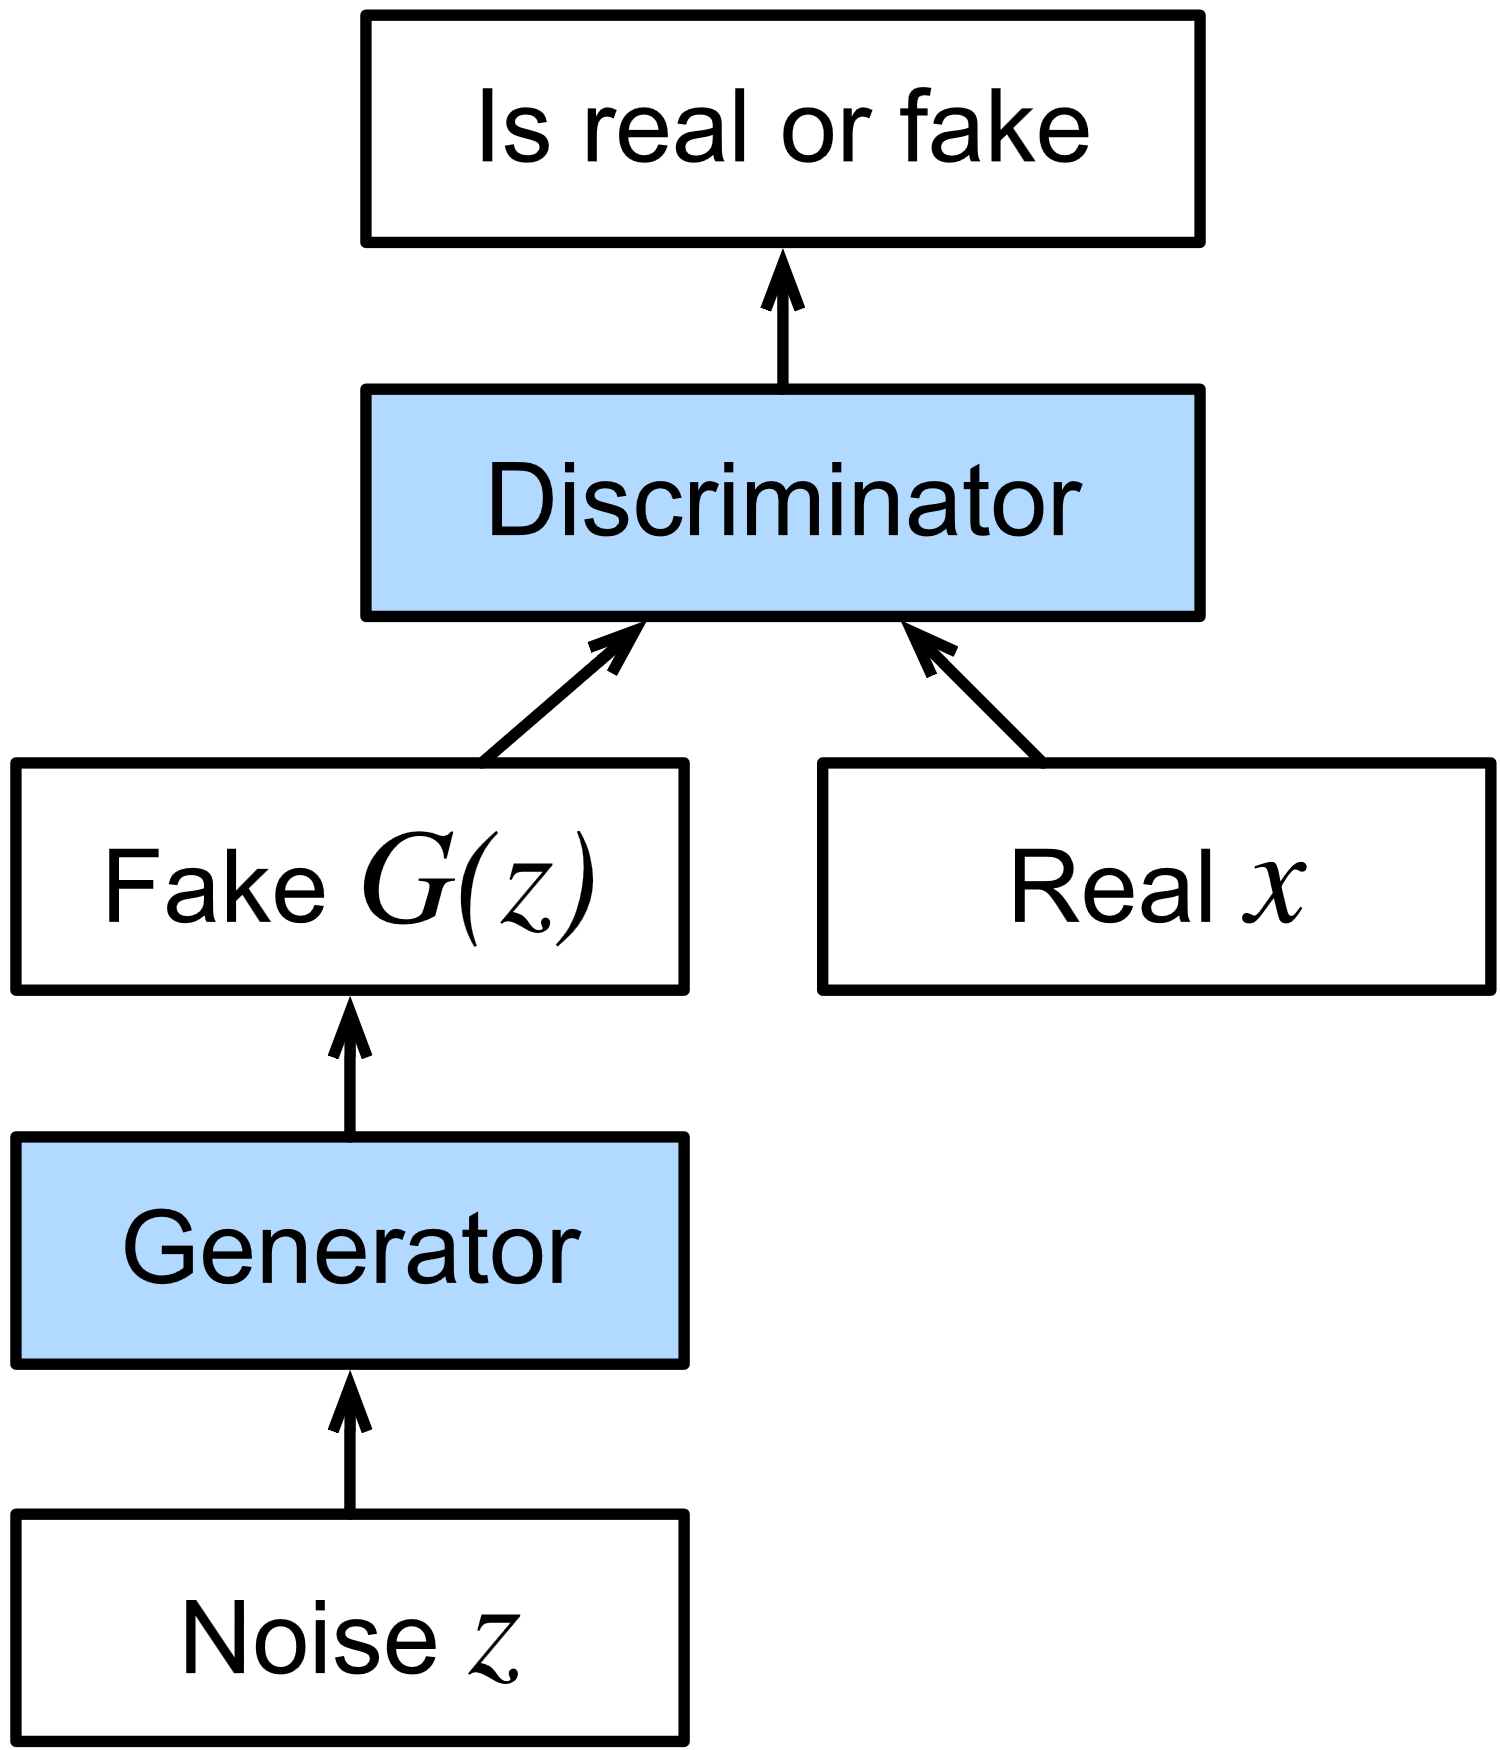
\includegraphics[width=\textwidth]{img/gan.png}
			\end{center}
		\end{column}
		\begin{column}{.6\textwidth}
			GANs have the following setup:

			\textbf{Discriminator} $f_\xi: \mathbb{R}^{C \times D_1 \times D_2} \rightarrow [0, 1]$
			\textbf{Generator} $G_\theta: \mathbb{R}^{Z} \rightarrow \mathbb{R}^{C \times D_1 \times D_2}$ \pause \newline \\

			The difference between generated and target distribution is minimized using divergences. \pause \newline \\

			\textbf{Q:} Are gradients always informative? \pause \\
			\textbf{A:} No; consider parallel lines infinitesimally close to one another. $KL = \infty,~JS = \log 2$ \pause \newline \\

			Instead, what if we use \textit{distance}? \pause \newline \\
			New \textbf{Discriminator} $f_\xi: \mathbb{R}^{C \times D_1 \times D_2} \rightarrow \mathbb{R}$
			which models Wasserstein Distance.
		\end{column}
	\end{columns}
\end{frame}

\begin{frame}{Training WGANs}
	\begin{algorithm}[H]
		\caption{WGAN training algorithm. $\eta = 10^{-5},~c=0.01,~n_{\text{critic}}=5,~n_{\text{iter}} = 500$.}\label{algo::wgan}
		\begin{algorithmic}[1]
			\For{$t = 0, ..., n_{\text{iter}}$}
			\For{$t = 0, ..., n_{\text{critic}}$}
			\State Sample $\{x_i\}_{i=1}^B \sim \mathcal{D}^B$ a batch from the real data.
			\State Sample $\{z_i\}_{i=1}^B \sim \mathcal{P}^B$ a batch of prior samples.
			\State $g_\xi \gets \nabla_\xi \left[\frac{1}{B}\sum_{i=1}^B f_\xi(x_i) - \frac{1}{B} \sum_{i=1}^B f_\xi(G_\theta(z_i)) \right]$
			\State $\xi \gets \xi + \eta \cdot \text{RMSProp}(g_\xi) $
			\State $\xi \gets \text{clip}(\xi, [-c, +c]) $
			\EndFor
			\State Sample $\{z_i\}_{i=1}^B \sim \mathcal{P}(z)$ a batch of prior samples.
			\State $g_\theta \gets -\nabla_\theta \frac{1}{B} \sum_{i=1}^B f_\xi(G_\theta(z_i))$ 
			\State $\theta \gets \theta - \eta \cdot \text{RMSProp}(g_\theta)$
			\EndFor
		\end{algorithmic}
	\end{algorithm}
\end{frame}

\begin{frame}{Critic Improvements from Wasserstein GANs}
	\begin{center}
		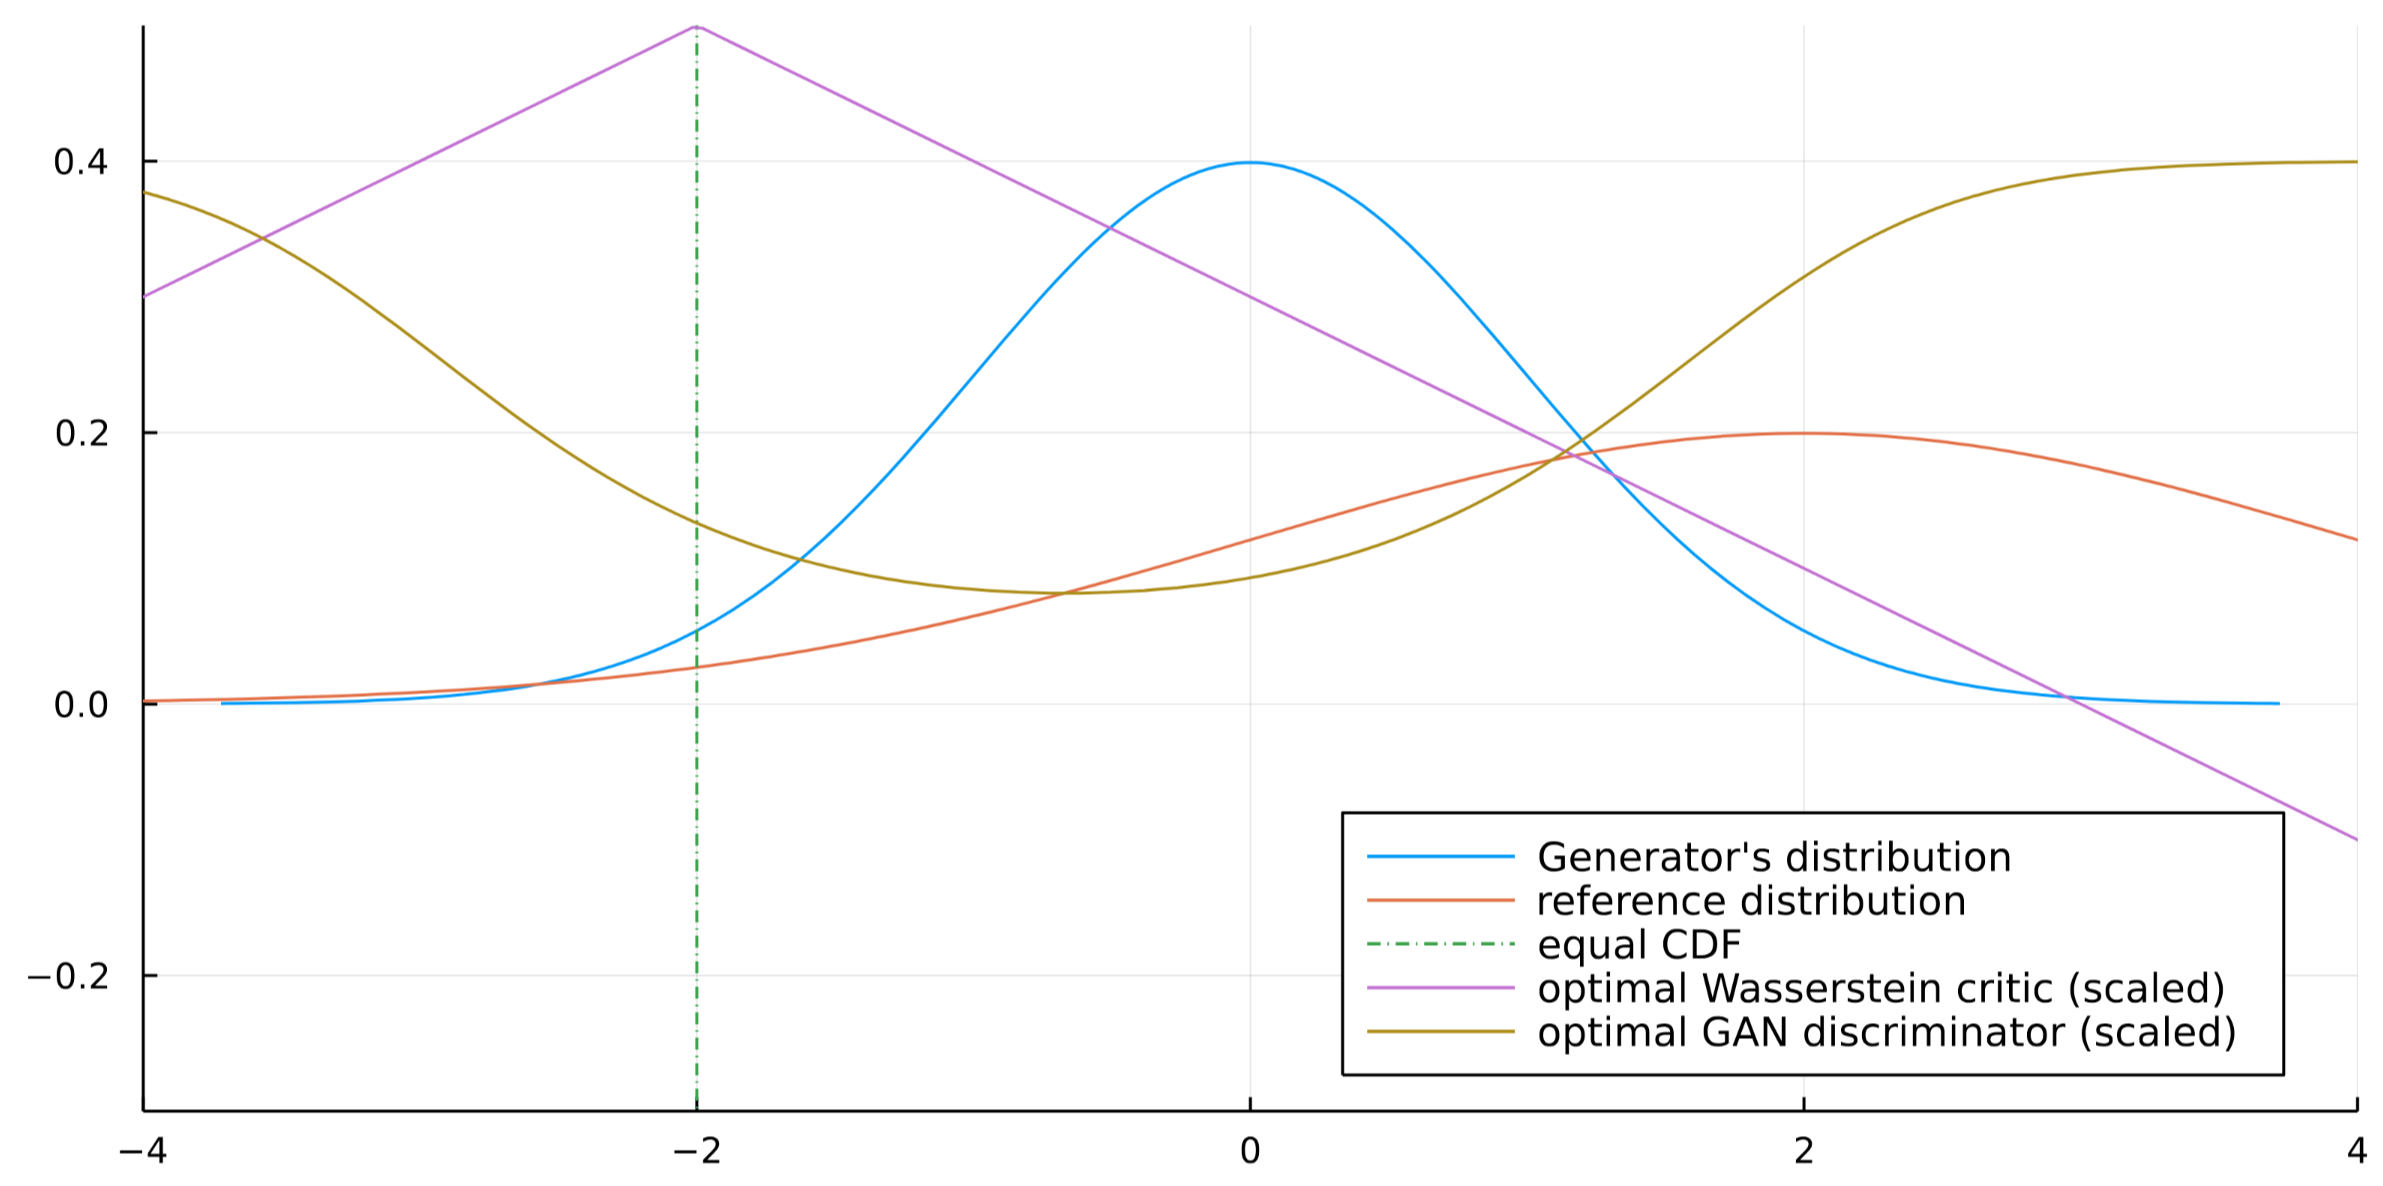
\includegraphics[width=\textwidth]{img/wgan_grad_compare.png}
	\end{center}
\end{frame}

\begin{frame}{Code Example -- Training WGANs}
	\begin{center}
		If you can view this screen, I am making a mistake.
	\end{center}
\end{frame}

\begin{frame}{Thank you!}
	\begin{center}
		Have an awesome rest of your day!
	\end{center}
	\begin{center}
		\textbf{Slides:} \url{https://jinen.setpal.net/slides/ot.pdf}
	\end{center}
\end{frame}

\end{document}
